\include{sections/Preamble/Preamble}

\begin{document}

\begin{titlepage}
\headheight = 57pt
\footskip = 5pt
\headsep = 0pt


{\begin{Large}
\university\\
\end{Large} }
\school\\
\department\\

\vspace*{5 cm}



\begin{Large}
\textbf{\doctitle}\\
\end{Large}
\docsubtitle\\
\me \quad (\studentcode)\\\\
{\small Wednesday 18$^\text{th}$ November, 2020}

\begin{flushright}
\textbf{Technical Supervisor}\\ \supervisor\\
\textbf{Academic Supervisors}\\\cosupervisor\\
\cocosupervisor
\end{flushright}

\vspace*{3cm}
\begin{figure}[h]
\centering
\begin{subfigure}{.5\textwidth}
  \centering
  \includegraphics[width=.5\linewidth]{images/utwente.png}
\end{subfigure}%
\begin{subfigure}{.5\textwidth}
  \centering
  \includegraphics[width=.4\linewidth]{images/nedap.png}
\end{subfigure}
\end{figure}





\vfill
\end{titlepage}


\begin{abstract}
FPGAs allow reconfiguration of its logic at any point after production. The result is that they are effective at prototyping application-specific integrated circuits, updating the internal logic while in the field and at low-cost low-quantity use cases. To optimise these processes, it is crucial to properly educate engineers in the implementation of FPGA programs and the FPGA compilation process. Traditional FPGA programming pipelines involve a computationally expensive (NP-hard) place \& route process that slows down iterations of FPGA programs and hinders the educational process. We propose a virtual environment in which place \& route is performed manually in which the student learns about the intricacies of place \& route and in which compilation is linear. To this end, we require emulation of a virtual FPGA on a physical, concrete FPGA. In the proposed research, we find such an emulation using an algorithm that solves a variant of subgraph isomorphism. This algorithm aims to find emulations in as many cases as possible and to exploit the hierarchy of FPGAs to speed up computation. The expected result is a software package that computes emulators which each output a program for a concrete FPGA provided with a program for a virtual FPGA.
\end{abstract}

\newpage
\tableofcontents
\chapter{Introduction}
Field Programmable Gate Arrays (FPGAs) play a significant role in the semiconductor industry. Because companies can configure the logic of these devices after mass hardware production, they can effectively use them for prototyping and emulation of Application Specific Integrated Circuits (ASICs). These are chips that are custom made for specific purposes and cannot be reconfigured. FPGAs can also be used to reconfigure program logic effectively, even while the hardware is in use. Moreover, the high computing performance for parallel calculations yielded by a small chip makes an FPGA suitable for sensor systems \cite{Garcia20146247}, cryptography\cite{Yalla2009225, Nawari2015, Ikram2020172}, digital signal processing\cite{4566369}, protocol implementations\cite{Saha2014} and other types of high-performance computing \cite{Kanazawa2010}.

We should adequately educate the engineers that implement FPGA programs to exploit their potential in this variety of problem areas. Usually, this is done by having students implement programs in a Hardware Description Language (HDL) such as VHDL or Verilog, compile it using FPGA vendor software to bit-level code that is written to FPGA hardware and execute it. This type of compilation takes a significant amount of time as the place \& route process required for compilation are both NP-complete problems \cite{1585279}. Another option is to simulate FPGA programs instead, which is the industry standard used for testing ASICs (non-programmable FPGAs). Simulation circumvents the place \& route process. However, simulation software run on a CPU has to simulate each component sequentially for each CPU core, resulting in enormous performance loss and thus a negative learning experience.

Another technique that could be used to execute an FPGA configuration is modelling the semantics of virtual FPGA components in an HDL module. The engineer can then simulate the execution of a virtual FPGA program by providing both the input \textit{and} configuration of these components as (stored) inputs to the hardware. An example of this is illustrated in Section \ref{sec:simulation} and Figure \ref{fig:simulation}. The trade-off here is that the hardware uses many resources for the simulation of each component. Because of this increased resource consumption, the performance of FPGA programs decreases as well. This technique is generally not used in the industry because of this reduced performance.

Techniques that require students to implement FPGA programs in HDLs furthermore abstract away the process of place \& route, a process that significantly affects the performance of the hardware implementation of the program. Since students should be educated to use this process optimally or even improve it, they should be aware of it and its underlying operations to build a bottom-up understanding of the entire FPGA engineering pipeline.

We propose an education environment where students implement program logic and place \& route manually in a simple, virtual FPGA. This way, the course designer has full control over the learning environment without being constrained to physical hardware. Performing the NP-complete place \& route manually allows the rest of the compilation process to take linear time, providing a configuration for the virtual FPGA. We aim to devise a method to compile this configuration for a virtual FPGA to a configuration compatible with a concrete one in linear time.

This way, students can circumvent the time-consuming compilation from HDLs to FPGAs, resulting in faster iterations and improved learning experiences. Furthermore, students can use this environment to learn the inherent difficulty of place \& route before they use tools that encapsulate this process in a `black box'. They will have to do this when they implement more complex structures in the virtual environment.

We can achieve this emulation by calculating a \textit{mapping} from the configuration of a virtual FPGA to the configuration of a real-life FPGA board (concrete FPGA). This mapping retains the semantics of the configuration but makes it suitable for execution on real hardware. While the format of an FPGA configuration is usually kept secret by hardware vendors \cite{Hauck:2007:RCT:1564780, 8653869, 6339165}, some FPGA boards have been reverse engineered to reveal the underlying format \cite{Yu2018, trellis}. Once this technique has been implemented and tested on those FPGAs, It can be put in practice in lab sessions of colleges and universities. Moreover, vendors can implement it for undisclosed FPGA designs and configuration formats as well for educational purposes as well.

%This research applies a space-efficient variant of Xiao's algorithm \cite{XIAONODEDISJOINT} for the graph problem `subgraph homeomorphism': an embedding of some source graph in a target graph, where addition of intermediate vertices is permitted. Applying this algorithm to graph models of FPGA provides such a mapping. We furthermore improve this algorithm using various methods from the domain of subgraph isomorphism (a similar graph problem), evaluate the different settings/improvements of this algorithm and how practical this algorithm is for educational use cases. 

Another use case of such mappings is synthesis of the same configuration to many hardware FPGA devices. Using our technique, synthesis of some FPGA program only has to take place once (to a virtual FPGA) before suitable configurations can be retrieved for many hardware architectures. Other applications may also benefit from this research when viewing partial FPGA emulation as a form of pre-compilation: performing FPGA compilation as much as possible without the knowledge of some aspects of the configuration. If this research is extended to include other forms of partial compilation, it may be used to improve the speed of general iterations of FPGA development as well.

The goals of this research are specified in Chapter \ref{sec:Objectives} (Objectives). This is a more specific description of the problem we outlined in this introduction requiring little background information. In Chapter \ref{sec:background} (Background) we will provide background on FPGAs and the graph problem `subgraph homeomorphism': a graph problem we will use to reach our objectives. In Chapter \ref{chapter:models} (Models) we specify how we model FPGAs as graphs to make them applicable for subgraph homeomorphism. In Chapter \ref{chapter:algorithm} (Algorithm) we describe the algorithm we use to solve the subgraph homeomorphism with these graphs. We prune the search space with methods described in Chapter \ref{chapter:pruning} (Pruning). We perform experiments with models and the algorithm with different settings in Chapter \ref{chapter:experiments} (Experiments), followed by a discussion (Chapter \ref{chapter:discussion}) interpreting the results and a conclusion in Chapter \ref{chapter:conclusion}.
\chapter{Background}
\label{sec:background}
\section{FPGAs}
\begin{figure}
\centering
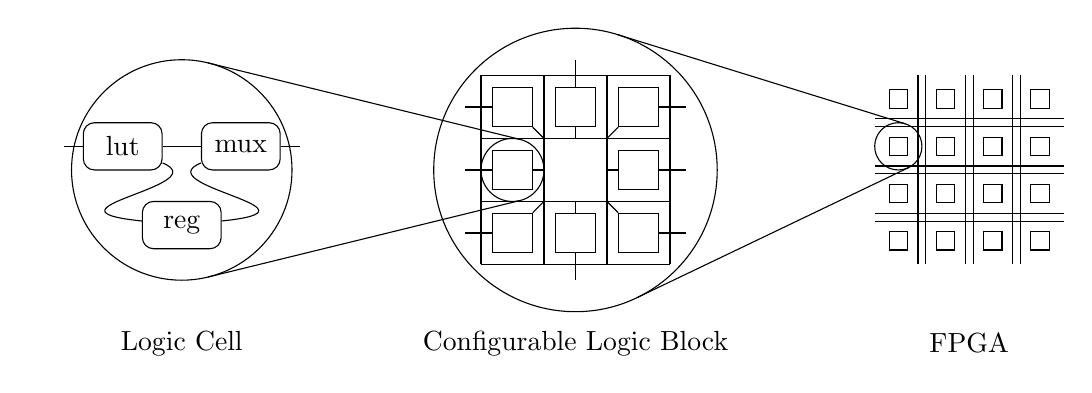
\begin{tikzpicture}
	\pgfmathsetmacro{\xone}{0}
	\pgfmathsetmacro{\xtwo}{5}
    \pgfmathsetmacro{\xthree}{10}
    
    \node [circle, draw] (cone) at (\xone,1.7) [minimum size=2.8cm] {};
    \node [circle, draw] (ctwo) at (\xtwo-0.8, 1.7) [minimum size=0.8cm] {};
\draw (0.33333333333333326, 3.0597385369580756)--(4.295238095238095, 2.0884967248451645);
\draw (0.33333333333333326, 0.34026146304192406)--(4.295238095238095, 1.3115032751548354);

    
    \draw (\xtwo, 1.7) circle (1.8cm);
    \draw (\xthree-0.9, 1.7+0.3) circle (0.3cm);
    \draw (5.532729751800444, 3.4193600587272686)--(9.18878829196674, 2.286560009787878);
\draw (5.777329419797189, 0.07649792943841183)--(9.229554903299531, 1.7294163215730687);
    
    \draw (\xone, -0.5) node {Logic Cell};
    \draw (\xtwo, -0.5) node {Configurable Logic Block};
    \draw (\xthree, -0.5) node {FPGA};


	\draw (\xone-0.75,2) node[rectangle, rounded corners, draw=black,minimum height=0.6cm, minimum width=1cm] (lut) {lut};
	\draw (\xone,1) node[rectangle, rounded corners, draw=black,minimum height=0.6cm, minimum width=1cm] (reg) {reg};
	\draw (\xone+0.75,2) node[rectangle, rounded corners, draw=black,minimum height=0.6cm, minimum width=1cm] (mux) {mux};
	
	\draw (lut)..controls (\xone+0.45,1.5) and (\xone-1.95, 1.2)..(reg);
	\draw (mux)..controls (\xone-0.45,1.5) and (\xone+1.95, 1.2)..(reg);
	\draw (lut)--(mux);
	\draw (lut)--(\xone-1.5,2);
	\draw (mux)--(\xone+1.5,2);
	
	

	
	
	\draw (\xtwo-0.8, 2.5) node[rectangle, draw=black, minimum height = 0.5cm, minimum width=0.5cm] (n1) {};
	
	\draw (\xtwo, 2.5) node[rectangle, draw=black, minimum height = 0.5cm, minimum width=0.5cm] (n2) {};
	
	\draw (\xtwo+0.8, 2.5) node[rectangle, draw=black, minimum height = 0.5cm, minimum width=0.5cm] (n3) {};
	
	\draw (\xtwo-0.8, 1.7) node[rectangle, draw=black, minimum height = 0.5cm, minimum width=0.5cm] (n4) {};
	
	\draw (\xtwo+0.8, 1.7) node[rectangle, draw=black, minimum height = 0.5cm, minimum width=0.5cm] (n5) {};
	
	\draw (\xtwo-0.8, 0.9) node[rectangle, draw=black, minimum height = 0.5cm, minimum width=0.5cm] (n6) {};
	
	
	\draw (\xtwo, 0.9) node[rectangle, draw=black, minimum height = 0.5cm, minimum width=0.5cm] (n7) {};
	
	
	\draw (\xtwo+0.8, 0.9) node[rectangle, draw=black, minimum height = 0.5cm, minimum width=0.5cm] (n8) {};
	
	\draw(\xtwo-1.2,2.9)--(\xtwo-1.2,0.5);
	\draw(\xtwo-0.4,2.9)--(\xtwo-0.4,0.5);
	\draw(\xtwo+0.4,2.9)--(\xtwo+0.4,0.5);
	\draw(\xtwo+1.2,2.9)--(\xtwo+1.2,0.5);
	
	\draw(\xtwo-1.2,2.9)--(\xtwo+1.2,2.9);
    \draw(\xtwo-1.2,2.1)--(\xtwo+1.2,2.1);
    \draw(\xtwo-1.2,1.3)--(\xtwo+1.2,1.3);
    \draw(\xtwo-1.2,0.5)--(\xtwo+1.2,0.5);
    
    %Lines from logic cells to the inside
    \draw(n1)--(\xtwo-0.4,2.1);
    \draw(n2)--(\xtwo,2.1);
    \draw(n3)--(\xtwo+0.4,2.1);
    \draw(n4)--(\xtwo-0.4,1.7);
    \draw(n5)--(\xtwo+0.4,1.7);
    \draw(n6)--(\xtwo-0.4,1.3);
    \draw(n7)--(\xtwo,1.3);
	\draw(n8)--(\xtwo+0.4,1.3);
	
   %Lines from logic cells to the outside;
   \draw(n1)--(\xtwo-1.4, 2.5);
   \draw(n2)--(\xtwo, 3.1);
   \draw(n3)--(\xtwo+1.4, 2.5);
   \draw(n4)--(\xtwo-1.4, 1.7);
   \draw(n5)--(\xtwo+1.4, 1.7);
   \draw(n6)--(\xtwo-1.4, 0.9);
   \draw(n7)--(\xtwo, 0.3);
   \draw(n8)--(\xtwo+1.4, 0.9);
   
   
   \draw (\xthree-0.9, 1.7+0.9) node[rectangle, draw=black] (sn1) {};
   \draw (\xthree-0.3, 1.7+0.9) node[rectangle, draw=black] (sn2) {};
   \draw (\xthree+0.3, 1.7+0.9) node[rectangle, draw=black] (sn3) {};
   \draw (\xthree+0.9, 1.7+0.9) node[rectangle, draw=black] (sn4) {};   
   
   \draw (\xthree-0.9, 1.7+0.3) node[rectangle, draw=black] (sn5) {};
   \draw (\xthree-0.3, 1.7+0.3) node[rectangle, draw=black] (sn6) {};
   \draw (\xthree+0.3, 1.7+0.3) node[rectangle, draw=black] (sn7) {};
   \draw (\xthree+0.9, 1.7+0.3) node[rectangle, draw=black] (sn8) {};
   
   \draw (\xthree-0.9, 1.7-0.3) node[rectangle, draw=black] (sn9) {};
   \draw (\xthree-0.3, 1.7-0.3) node[rectangle, draw=black] (sn10) {};
   \draw (\xthree+0.3, 1.7-0.3) node[rectangle, draw=black] (sn11) {};
   \draw (\xthree+0.9, 1.7-0.3) node[rectangle, draw=black] (sn12) {};
   
   \draw (\xthree-0.9, 1.7-0.9) node[rectangle, draw=black] (sn13) {};
   \draw (\xthree-0.3, 1.7-0.9) node[rectangle, draw=black] (sn14) {};
   \draw (\xthree+0.3, 1.7-0.9) node[rectangle, draw=black] (sn15) {};
   \draw (\xthree+0.9, 1.7-0.9) node[rectangle, draw=black] (sn16) {};
   
   \draw (\xthree-0.05, 1.7+1.2)--(\xthree-0.05, 1.7-1.2);
   \draw (\xthree+0.05, 1.7+1.2)--(\xthree+0.05, 1.7-1.2);
   \draw (\xthree+0.6-0.05, 1.7+1.2)--(\xthree+0.6-0.05, 1.7-1.2);
   \draw (\xthree+0.6+0.05, 1.7+1.2)--(\xthree+0.6+0.05, 1.7-1.2);
   \draw (\xthree-0.6-0.05, 1.7+1.2)--(\xthree-0.6-0.05, 1.7-1.2);
   \draw (\xthree-0.6+0.05, 1.7+1.2)--(\xthree-0.6+0.05, 1.7-1.2);
   
   \draw (\xthree+1.2, 1.7+0.05)--(\xthree-1.2, 1.7+0.05);
   \draw (\xthree+1.2, 1.7-0.05)--(\xthree-1.2, 1.7-0.05);
   \draw (\xthree+1.2, 1.7+0.6+0.05)--(\xthree-1.2, 1.7+0.6+0.05);
   \draw (\xthree+1.2, 1.7+0.6-0.05)--(\xthree-1.2, 1.7+0.6-0.05);
   \draw (\xthree+1.2, 1.7-0.6+0.05)--(\xthree-1.2, 1.7-0.6+0.05);
   \draw (\xthree+1.2, 1.7-0.6-0.05)--(\xthree-1.2, 1.7-0.6-0.05);

	
\end{tikzpicture}
\caption{The hierarchy of a typical FPGA. A typical FPGA mostly consists of Configurable Logic Blocks (CLBs) and a CLB mostly consists of logic cells. The way logic cells and CLBs are connected may be different for each FPGA architecture.}
\end{figure}


The computing hardware most people are familiar with is CPUs. Manufacturers incorporate them in every desktop pc, laptop, and most mobile devices. CPUs are very flexible and efficient- which is why they are the de facto standard for any computation task. In CPU computation, an integrated circuit (a processor) iteratively reads an instruction from a RAM module (in the form of encoded bits), performs the instruction, and then continues to read the next instruction. The instructions are not embedded in the circuit of the CPU itself.

FPGAs are different from CPUs, as they do not store the programs they execute in RAM- they instead configure them in the (highly parallel) logic of the circuit itself. Configuring an FPGA to execute a specific program entails loading a configuration file onto the hardware and restarting the FPGA such that it reconfigures its logic. The hardware will then perform the configured logic on the input it receives via IO pins. 

Because each logic cell performs logic independently, FPGAs can perform computations highly parallel and without delays from sequentially loading instructions. This computation process implies that FPGAs are very efficient at executing concurrent programs. Reconfiguring an FPGA is, however, a relatively expensive operation. Therefore, FPGAs are unsuitable for changing from program to program, as a CPU does when running an operating system. Moreover, FPGAs can be slower than CPUs for nonparallel applications since its longer critical path length (i.e. distance an electric current has to travel each clock cycle) results in a lower clock speed. Lastly, the different structure of an FPGA requires programs for them to be developed in specialized HDL languages instead of CPU-based programming languages, although efforts are being made to bring these domains closer together.

FPGAs perform execution using components such as lookup tables, registers, and special-purpose modules\footnote{These modules are used for efficient storage or calculation of specific functions. We will disregard them in this research.}. These components are physical structures on the circuit. In the next sections, we will discuss these modules.
\subsection{Lookup tables}


\begin{figure}
\centering
\begin{tabular}{|c|c|c|}
\hline
$p$ & $q$ & $p$ XOR $q$ \\ \hline
$F$ & $F$ & $F$       \\ \hline
$F$ & $T$ & $T$       \\ \hline
$T$ & $F$ & $T$       \\ \hline
$T$ & $T$ & $F$       \\ \hline
\end{tabular}
\caption{A truth table that shows the result of an XOR operation}
\label{fig:truth_table}
\end{figure}

\begin{figure}
\centering
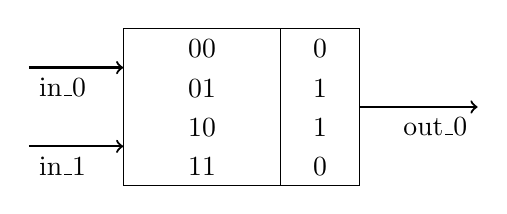
\begin{tikzpicture}
    \draw (0,0) rectangle (3,2);
    \draw (2, 0) -- (2, 2);
    \draw[thick,->] (-1.2,0.5) node[anchor=north west] {in\_1} -- (0,0.5);
    \draw[thick,->] (-1.2,1.5) node[anchor=north west] {in\_0} -- (0,1.5);
    
    \draw[thick,->] (3,1)  -- (4.5,1) node[anchor=north east] {out\_0};
    
    \draw[draw=white] (1,1.5)    node[anchor=south] {00};
    \draw[draw=white] (1,1)      node[anchor=south] {01};
    \draw[draw=white] (1,0.5)    node[anchor=south] {10};
    \draw[draw=white] (1,0)      node[anchor=south] {11};
    
    
    \draw[draw=white] (2.5,1.5)   node[anchor=south] {$0$};
    \draw[draw=white] (2.5,1)     node[anchor=south] {$1$};
    \draw[draw=white] (2.5,0.5)   node[anchor=south] {$1$};
    \draw[draw=white] (2.5,0)     node[anchor=south] {$0$};
\end{tikzpicture}
\caption{A Lookup Table (LUT) in which an XOR-operation is configured}
\label{fig:lookuptable}
\end{figure}

Any boolean logic formula can be expressed in the form of a truth table, such as in Figure \ref{fig:truth_table}. The leftmost column of a truth table specifies all possible combinations of $T$ and $F$ for all inputs; the rightmost column then specifies what output that specific logic function would give. Each distinct combination of $T$ and $F$ in the rightmost column corresponds to a different boolean formula. FPGAs execute logic in the form of Lookup Tables (LUTs), which model the evaluation of a truth table, but with ones and zeroes instead of $T$ and $F$: for every combination of ones and zeroes in the input, the LUT stores what output it should give. The compilation software provided by the FPGA vendor can reconfigure these outputs. This way, any boolean formula with the appropriate number of variables can be implemented with a lookup table. Figure \ref{fig:lookuptable} shows a lookup table that has two input bits and one output bit. This lookup table is configured to perform an XOR-operation. Lookup tables can have input and output consisting of any number of bits, depending on the FPGA design.

\subsection{Registers}
\begin{figure}
\centering
\begin{tikzpicture}
    \draw (0,0) rectangle (1.5,2);
    \draw[-{Latex[length=5mm, open]}] (-1.2,0.5) node [anchor=north west] {$clock$} -- (0.5,0.5);
    \draw[-{Latex[length=3mm]}] (-1.2,1.5) node[anchor=east] {$D$} -- (0,1.5);
    
    \draw (-1.2,1.6) -- (-0.8,1.6) -- (-0.5,1.5);
    \draw (-1.2,1.7) -- (-0.8,1.7) -- (-0.5,1.5);

    \draw (1.5, 1.1)--(1.9,1.1)--(2.2,1);
    \draw (1.5, 1.2)--(1.9,1.2)--(2.2,1);
    \draw[-{Latex[length=3mm]}] (1.5,1) -- (2.7,1) node[anchor=west] {$Q$};
\end{tikzpicture}
\caption{Traditional representation of a register. Note that input \textit{D} and output \textit{Q} may consist of multiple wires.}
\label{fig:register}
\end{figure}

Programs require intermediate data storage to perform any computation that is more complex than combinational logic.

FPGAs use registers for this purpose (see Figure \ref{fig:register}). Registers can store a small collection of bits, depending on the FPGA design. When a register's input $clock$ changes from 0 to 1, the contents of the register are replaced by the value of the input $D$, and the output $Q$ takes this value. The output stays constant until the clock changes from 0 to 1 again when D has a different value.

FPGAs usually have clocks- wires whose signal constantly changes between 0 and 1 that is connected to registers in the hardware. This can be a single global clock connected to each register or a network of clocks each responsible for different parts of the FPGA. The frequency of this clock is chosen such that all signals are guaranteed to be stable when the clock becomes 1. This stability is very convenient for programmers, who do not have to calculate the time it takes for a signal to propagate through a wire. The implication is that each circuit combining only lookup tables that end in the D-input of a register takes the same amount of time.

If the FPGA program has longer chains of lookup tables, then it takes longer for the output signal to stabilize. The vendor software accommodates for this by setting the global clock at a lower frequency. Since programs on FPGAs are highly parallel, there are likely some parts of the calculation that do not require a lower clock speed and can cause slowdown because of this. In these scenarios, adding registers to some parts of an FPGA program can improve performance if it allows the global clock speed to be higher.


\subsection{Logic cells}

\begin{figure}
\centering
\begin{tikzpicture}
	%Register
    \draw (0,0) rectangle (1.5,2);
    \draw[-{Latex[length=5mm, open]}] (-1.2,-1) node [anchor=south east] {$clock$} -- (-1.2,0.5) -- (0.5,0.5);
    
    %Line from Register to MUX
    \draw[-{Latex[length=3mm]}] (1.5,1) -- (2.7,1) -- (2.7, 2.333) -- (3.7, 2.333);
    \draw (1.5, 1.1) -- (1.9, 1.1) -- (2.1, 1);
    \draw (1.5, 1.2) -- (1.9, 1.2) -- (2.1, 1);
    \draw (2.56,1) -- (2.7, 1.14);
    \draw (2.42,1) -- (2.7, 1.28);
    \draw (2.7, 2.1933) -- (2.84, 2.333);
    \draw (2.7, 2.0533) -- (2.98, 2.333);
    
    %LUT
    \draw (-5,2) rectangle (-2,4);
    \draw (-3, 2) -- (-3, 4);

    \draw[-{Latex[length=3mm]}] (-6.5,3) node[anchor=north west] {in} -- (-5,3);
	\draw (-6.5, 3.1) -- (-6.1, 3.1);
	\draw (-6.5, 3.2) -- (-6.1, 3.2);
	\draw (-6.1, 3.1) -- (-5.9, 3);
	\draw (-6.1, 3.2) -- (-5.9, 3);
    
    
    
    %Line from LUT to Register
    \draw[-{Latex[length=3mm]}] (-2,3)  -- (-1.1,3) -- (-1.1, 1.5) -- (0,1.5);
	
	\draw (-2,3.1) -- (-1.6,3.1) -- (-1.4, 3);    
	\draw (-2,3.2) -- (-1.6,3.2) -- (-1.4, 3);

    \draw (-1.24, 3) -- (-1.1, 2.86);
    \draw (-1.38, 3) -- (-1.1, 2.72);
    \draw (-1.1, 1.64) -- (-0.96, 1.5);
    \draw (-1.1, 1.78) -- (-0.82, 1.5);
    
    
    %LUT keys
    \draw[draw=white] (-4,3.25) node[anchor=south] {$0000$};
    \draw[draw=white] (-4,2.75) node[anchor=south] {$\cdots$};
    \draw[draw=white] (-4,2.25) node[anchor=south] {$1111$};
    
    %LUT values
    \draw[draw=white] (-2.5,3.25) node[anchor=south] {$x_0$};
    \draw[draw=white] (-2.5,2.75) node[anchor=south] {$\cdots$};
    \draw[draw=white] (-2.5,2.25) node[anchor=south] {$x_n$};
    
    %Line from LUT to MUX
    \draw[-{Latex[length=3mm]}] (-2,3)  -- (3.7,3);
    
    %MUX
    \draw (3.7, 3.6667) -- (3.7, 1.6667) -- (4.7, 2.111) -- (4.7, 3.111) -- cycle;
    
    %M
    \draw[-{Latex[length=3mm]}] (2.2, 0.5) node[anchor=north west] {$m$} --(4.2, 0.5) -- (4.2, 1.8667);
    
    
    \draw[-{Latex[length=3mm]}] (4.7, 2.5) -- (6.2, 2.5) node[anchor = north east] {out};
    \draw (4.7, 2.6) -- (5.1, 2.6);
    \draw (4.7, 2.7) -- (5.1, 2.7);
    \draw (5.1, 2.6) -- (5.3, 2.5);
    \draw (5.1, 2.7) -- (5.3, 2.5);      

    
\end{tikzpicture}
\caption{An $n$-input logic cell. $x_k$ and $m$ must be configured for any $0 \leq k \leq n$}
\label{fig:logiccell}
\end{figure}

A typical logic cell is a combination of one or more lookup tables, a register, and a MUX (a 3-input gate that outputs a copy of the first or second input, depending on the value of the third input).  The contents of the lookup tables can be configured to perform any logic operation, and the value of the third MUX-input can be configured to specify whether the computation is clocked/synchronous or combinatorial/asynchronous. A logic cell is shown in Figure \ref{fig:logiccell}. Unfortunately for us, vendors have different logic cell designs, meaning we cannot generalize this example.

FPGA manufacturers often group Logic cells in Configurable Logic Blocks (CLB) that make hardware production, placement, and routing (Section \ref{sec:compilation}) easier.
 
The main building blocks of FPGAs are CLBs that are connected via routing fabric. These are responsible for most of the computation of FPGA programs. FPGAs can have additional modules such as RAM and Digital Signal Processors that optimize storage and specialized arithmetic, respectively. Each of these modules' functionality could also be performed by a collection of logic cells at the cost of performance. In this research, we will only consider CLBs.

\subsection{Routing}
A single logic cell can only perform simple programs such as logic gates. The FPGA needs to connect different logic cells to perform any kind of logic operation, dependent on what program it needs to execute. The way logic cells and other modules are connected on a physical FPGA in a specific configuration is called the \textbf{routing} of an FPGA. On the most basic level, FPGAs perform routing with configurable transistors. These are tiny modules on an FPGA board that are connected with an input wire and an output wire. They can be configured to allow electric current flowing from its input to its output or to block any incoming electric current.

\subsection{Pins}
To supply the FPGA with input and to allow it to provide output, an FPGA is equipped with a set of metal pins. Each of those pins is connected with a wire on the FPGA board. Each pin can be used for either input or output, depending on the configured program. For example, an FPGA used to control an electric stepper motor will receive input with the requested motor speed and direction and will output signals to specific circuits that need to be activated to obtain that speed and direction.




\section{FPGA compilation}
\label{sec:compilation}
To program an FPGA, an engineer has to specify a hardware design that describes the semantics of the program. They write these hardware designs in a Hardware Description Language (HDL). Commonly used languages for this purpose are VHDL and Verilog. They specify on an abstract level what functionality the program should have, preferably in a modular structure to improve maintainability.

The software then needs to translate this abstract description to a \textbf{netlist}: a description of logic, registers, specialized components, and how they are connected. Depending on the configuration of the compilation software, this netlist may undergo a sequence of optimisations and transformations between several levels of abstraction. This process is called \textbf{synthesis}; beware though that some sources call the entire FPGA compilation process synthesis.

The next step in the compilation process is \textbf{placement}. The software maps each LUT, register, and other components to a physical place on the FPGA. The software can place components closer together to optimize the speed or can place components further apart to increase the probability routes can be found. Finding the optimal placement for speed is a proven NP-hard problem.

The last step in the compilation process is \textbf{routing}. State-of-the-art FPGA compilation pipelines perform this step sequentially after placement\cite{alhyari2019}. With the components locked in place, the software attempts to find a configuration of routing switches such that each connection that the synthesis requires is made. Finding the optimal routes for speed is an NP-hard problem while finding any matching routing configuration is an NP problem. Both can be reducted to the problem of fixed-vertex subgraph homeomorphism of which the optimisation variant needs to explore the entire search tree, which \cite{ExactComplexity} showed can be computed in $O(2^{|T|-|S|}n^{O(1)})$ for the general case. However, routing algorithms are often made for specific FPGA architectures, allowing for better heuristics and thus performance.

\begin{minipage}{\textwidth}
\begin{important}
Note that place \& route of an FPGA \textit{program} as described here is a very similar problem to the emulation an unconfigured virtual FPGA to a concrete FPGA (this research). However, it is important to note that these are different problems: with place \& route, a mapping is obtained from a model of an \textit{FPGA program} to the concrete FPGA. In our research, we obtain a mapping from a model of a \textit{virtual FPGA} to the concrete FPGA. The two problems are on different levels of abstraction: an FPGA program does not have the concept of unconfigured components or transistors while a virtual FPGA does.

\vspace{.6cm}
Placement of FPGA programs using place \& route could theoretically also work on a higher abstraction level, i.e. including unconfigured components. The problem with this approach is that state-of-the art place \& route pipelines perform these algorithms sequentially: they perform placement based on speed- and routeability heuristics without a guarantee that the placement can indeed be routed \cite{alhyari2019}. With the placement of FPGA programs, this is not a problem. They are usually modular with components that have relatively few interconnecting wires. FPGAs, however, can consist of densely connected components that can severely impact routeability. We leave the analysis of place \& route algorithms for compatibility with FPGA-on-FPGA emulation for future research.
\end{important}
\end{minipage}


\begin{figure}
    \centering
\begin{tikzpicture}
    \draw (0,0) rectangle (3,2);
    \draw (2, 0) -- (2, 2);
    \draw[thick,->] (-1.2,0.5) node[anchor=north west] {in\_2} -- (0,0.5);
    \draw[thick,->] (-1.2,1.5) node[anchor=north west] {in\_1} -- (0,1.5);
    
    \draw[thick,->] (3,1)  -- (4,1) node[anchor=north] {out\_1};
    
    \draw[draw=white] (1,1.5)     node[anchor=south] {00};
    \draw[draw=white] (1,1)       node[anchor=south] {01};
    \draw[draw=white] (1,0.5)     node[anchor=south] {10};
    \draw[draw=white] (1,0)       node[anchor=south] {11};
    
    
    \draw[draw=white] (2.5,1.5)    node[anchor=south] {$x_0$};
    \draw[draw=white] (2.5,1)      node[anchor=south] {$x_1$};
    \draw[draw=white] (2.5,0.5)    node[anchor=south] {$x_2$};
    \draw[draw=white] (2.5,0)      node[anchor=south] {$x_3$};
    
    

     \draw (8,-1) rectangle (11,3);
    \draw (10, -1) -- (10, 3);
    \draw[thick,->] (6.8,0) node[anchor=north west] {in\_2} -- (8,0);
    \draw[thick,->] (6.8,1) node[anchor=north west] {N/A} -- (8,1);    
    \draw[thick,->] (6.8,2) node[anchor=north west] {in\_1} -- (8,2);
    
    \draw[thick,->] (11,1.5)  -- (12,1.5) node[anchor=north] {out\_1};
    \draw[thick,->] (11,0.5)  -- (12,0.5) node[anchor=north] {0};
    
	\draw[draw=white] (9,2.5)        node[anchor=south] {000};
    \draw[draw=white] (9,2)          node[anchor=south] {001};    
    \draw[draw=white] (9,1.5)        node[anchor=south] {010};
    \draw[draw=white] (9,1)          node[anchor=south] {011};
    \draw[draw=white] (9,0.5)        node[anchor=south] {100};
    \draw[draw=white] (9,0)          node[anchor=south] {101};
    \draw[draw=white] (9,-0.5)        node[anchor=south] {110};
    \draw[draw=white] (9,-1)          node[anchor=south] {111};
    
    
    \draw[draw=white] (10.5,2.5)         node[anchor=south] {$x_0 0$};
    \draw[draw=white] (10.5,2)           node[anchor=south] {$x_1 0$};    
    \draw[draw=white] (10.5,1.5)         node[anchor=south] {$x_0 0$};
    \draw[draw=white] (10.5,1)           node[anchor=south] {$x_1 0$};
    \draw[draw=white] (10.5,0.5)         node[anchor=south] {$x_2 0$};
    \draw[draw=white] (10.5,0)           node[anchor=south] {$x_3 0$};
    \draw[draw=white] (10.5,-0.5)         node[anchor=south] {$x_2 0$};
    \draw[draw=white] (10.5,-1)           node[anchor=south] {$x_3 0$};
    
    \draw[vecArrow] (5.5,1) -- (6.5,1);

\end{tikzpicture}
    \caption{Emulation of an FPGA: the configuration of the virtual FPGA is reflected in the configuration of the concrete FPGA. Any extra inputs and outputs are unused.}
    \label{fig:emulation}
    \vspace{1cm}
    \begin{tikzpicture}
    \draw (0,0) rectangle (3,2);
    \draw (2, 0) -- (2, 2);
    \draw[thick,->] (-1.2,0.5) node[anchor=north west] {in\_2} -- (0,0.5);
    \draw[thick,->] (-1.2,1.5) node[anchor=north west] {in\_1} -- (0,1.5);
    
    \draw[thick,->] (3,1)  -- (4,1) node[anchor=north west] {out\_1};
    
    \draw[draw=white] (1,1.5)    node[anchor=south] {00};
    \draw[draw=white] (1,1)      node[anchor=south] {01};
    \draw[draw=white] (1,0.5)    node[anchor=south] {10};
    \draw[draw=white] (1,0)      node[anchor=south] {11};
    
    
    \draw[draw=white] (2.5,1.5)     node[anchor=south] {$x_0$};
    \draw[draw=white] (2.5,1)       node[anchor=south] {$x_1$};
    \draw[draw=white] (2.5,0.5)     node[anchor=south] {$x_2$};
    \draw[draw=white] (2.5,0)       node[anchor=south] {$x_3$};
    
    

    \draw (8,-1.5) rectangle (11,2);
    \draw (10, -1.5) -- (10, 2);
	
	\draw[thick,->] (6.8,1.9) node[anchor=north west] 	{$x_0$} -- (8,1.9);
	\draw[thick,->] (6.8,1.3) node[anchor=north west] 	{$x_1$} -- (8,1.3);
	\draw[thick,->] (6.8,0.7) node[anchor=north west] 	{$x_2$} -- (8,0.7);
	\draw[thick,->] (6.8,0.1) node[anchor=north west] 	{$x_3$} -- (8,0.1);
	\draw[thick,->] (6.8,-0.5) node[anchor=north west] 	{in\_1} -- (8,-0.5);
    \draw[thick,->] (6.8,-1.1) node[anchor=north west] 	{in\_2} -- (8,-1.1);

    
    \draw[thick,->] (11,1)  -- (12,1) node[anchor=north west] {out\_1};
    
    \draw[draw=white] (9,1.5)       node[anchor=south] {000000};
    \draw[draw=white] (9,1)         node[anchor=south] {000001};
    \draw[draw=white] (9,0.5)       node[anchor=south] {000010};
	\draw[draw=white] (9,0)         node[anchor=south] {$\cdots$};
    \draw[draw=white] (9,-0.5)      node[anchor=south] {111101};
    \draw[draw=white] (9,-1) 	    node[anchor=south] {111110};
    \draw[draw=white] (9,-1.5)      node[anchor=south] {111111};
    
    
    
    \draw[draw=white] (10.5,1.5)         node[anchor=south] {$0$};
    \draw[draw=white] (10.5,1)           node[anchor=south] {$0$};
    \draw[draw=white] (10.5,0.5)         node[anchor=south] {$0$};
	\draw[draw=white] (10.5,0)           node[anchor=south] {$\cdots$};
	\draw[draw=white] (10.5,-0.5)        node[anchor=south] {$1$};
	\draw[draw=white] (10.5,-1)          node[anchor=south] {$1$};
	\draw[draw=white] (10.5,-1.5)        node[anchor=south] {$1$};
    
    
    \draw[vecArrow] (5.5,1) -- (6.5,1);

\end{tikzpicture}
    \caption{Simulation of an FPGA: the programming of the virtual FPGA is reflected in \textit{additional input} of the actual FPGA originating from some sort of explicit configuration source, e.g. RAM or a storage device connected to the concrete FPGA's input pins. The configuration of the concrete FPGA does \textit{not} depend on the configuration of the virtual FPGA and additional logic- and storage resources are used.}
    \label{fig:simulation}
\end{figure}

\section{The FPGA virtual machine}
\label{sec:simulation}
In this research, we will not be implementing an FPGA virtual machine. However, for clarity, we will explain what we mean it. Imagine a software engineer wants to execute a program $P$. Conventionally, they would program $P$ in an HDL, compile it to an FPGA configuration file and load it onto the hardware.

To instead simulate the synthesized program, the engineer can also program a generic FPGA environment in an HDL, compile it to an FPGA configuration file and load it onto the hardware. They can afterwards provide $P$ as \textit{input} to the program instead of using $P$ \textit{as} a program. This way, the virtual FPGA can run in a ``virtual machine" on the concrete FPGA. The \textit{static} configuration of the virtual FPGA uses the \textit{dynamic} resources (e.g. RAM and registers) of the concrete FPGA. A virtual machine of a single LUT is shown in Figure \ref{fig:simulation}.

Although engineers could use FPGA virtual machines to execute FPGA programs on FPGA hardware that the FPGA software was not compiled for, it introduces a considerable delay in execution. After all, many more dynamic components on the FPGA need to be used to store and execute the configuration of the same program.	



\section{FPGA emulation}
Instead, our research entails finding out how we can perform \textit{emulation}. With this, we mean the execution of a program on a different FPGA \textit{such that no extra input is required.} Instead, the emulator software inspects the program for the virtual FPGA and generates what program on the concrete FPGA would have the same semantics given the same inputs as the source FPGA. Figure \ref{fig:emulation} shows the emulation counterpart of Figure \ref{fig:simulation} with a smaller LUT. Since the target FPGA has one more input than the virtual FPGA, that input remains unused. Similary, since it has one more output, that output remains unused (i.e. always outputs 0). The configuration of the LUT is such that it has the same semantics as the virtual LUT with these constraints in mind. We aim to find out how we can perform this kind of emulation with any program with any fixed source- and destination FPGA whenever such emulation is possible.

\input{sections/Background/SimuEmu/SimuEmu}
\section{Graph theory}
Because of the network structure of FPGAs, it is easy to model them as graphs. If we model FPGA components as combinations of vertices and connections, we have a complete representation of an FPGA suitable for graph algorithms.

A graph representation of the physical structure of FPGAs allows us to scan through the structure of the concret FPGA graph and look for structures that resemble the graph of the virtual FPGA. Let us, for example, assume that the structure of the concrete FPGA graphs contains a complete embedding of the virtual FPGA graph. Then, by disabling each component outside of this embedding and by copying configurations from components in the virtual FPGA model to their respective components in the concrete FPGA graph model we would have an emulation function. This could entail changing some bits if, for example, the second output of a virtual LUT is mapped the the first output of the concrete LUT and vica versa.\footnote{While virtual components may also be emulated by structures of multiple concrete components connected in specific ways, we deem finding such emulations out of scope for this research.}

The graph theoretic name for finding these embeddings is subgraph isomorphism. It is an NP-complete problem\cite{cook} with many algorithms explored. The problem with using an approach of subgraph isomorphism is, however, that many possible emulations cannot be found. For example, a concrete FPGA may have much more configurable routing switches than an virtual FPGA. A subgraph isomorphism algorithm would in this case not find an emulation, even though one is technically possible by configuring some routing switches to function as wires.

A variant of subgraph isomorphism is (vertex disjoint) subgraph homeomorphism. In this problem, intermediate vertices are allowed in the embedding on the target-graph side. This means that the embedding consists of a vertex-to-vertex mapping and an edge-to-path mapping.

This is the essence of our research: finding some subset of the concrete FPGA (using graphs) that is topologically the same way as the virtual FPGA and has the appropriate components that can emulate virtual components one-to-one.

\begin{defn}[graph]
A graph is a tuple $(V, E, L)$ where $V$ is a set of vertices, $E$ is a multiset of directed edges such that each edge $e \in E \to e \in (V \times V)$ and $L: (V \to \mathbb{P}(\lambda))$ is a multilabelling function where $\lambda$ is a finite alphabet.
\label{def:graph}
\end{defn}


\begin{defn}[(vertex disjoint) subgraph homeomorphism]
Let $P$ the set of all loopless paths in $G_T$, let $\mathit{first}(p)$ be the first vertex of a path $p$, let $\mathit{last}(p)$ be the last vertex of a path $p$ and let $\mathit{intermediate}(p)$ be all other vertices of a path $p$. Then, a subgraph homeomorphism from graph $S$ to graph $T$ is a tuple $(\mathit{vmap}, \mathit{emap})$ where $\mathit{vmap}\subseteq (V_S \mapsto V_T)$ and $\mathit{emap} \subseteq (E_S \mapsto P)$ are both injective functions such that:

\begin{tabular}{rlr}
 1. & $\forall s \in V_S . L_S(s)\subseteq L_T(\mathit{vmap}(s))$&\\
 
 &i.e. vertices are mapped to vertices that have at least the same label set.&\\
 
 2. & $\forall (s_1, s_2) \in E_S .\mathit{first}(\mathit{emap}(s_1, s_2))=\mathit{vmap}(s_1) \land \mathit{last}(\mathit{emap}(s_1, s_2))=\mathit{vmap}(s_2)$&\\
 &i.e. each edge in $G_1$ is mapped to a path in $G_2$.&\\
 
 3. & $\forall p \in \mathit{values}(\mathit{emap}) . \forall x \in \mathit{intermediate}(p) . $\\
 &$\quad \not \exists p' \in (\mathit{values}(\mathit{emap}) \setminus \{p\}) . x \in \mathit{intermediate}(p')$&\\
    &i.e. these paths are internally vertex disjoint.&\\
\end{tabular}

This tuple is also the certificate for the decision problem of subgraph homeomorphism, which returns whether a tuple like this exists. A popular different way to define the decision problem is whether the target graph contains a subgraph which can be obtained by repeatedly intersecting the source graph's edges with vertices.

\label{def:pathsubgraphisomorphism}
\end{defn}


\begin{figure}
\centering
\parbox{1.2in}{

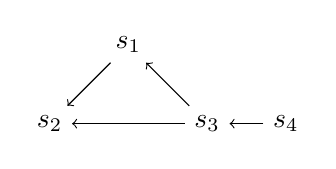
\begin{tikzpicture}
\node at (0,1) (a) {$s_1$};
\node at (1,0) (c)  {$s_3$};
\node at (-1,0) (b)  {$s_2$};
\node at (2,0) (d)  {$s_4$};

\draw[->] (a)->(b);
\draw[->] (c)->(a);
\draw[->] (c)->(b);
\draw[->] (d)->(c);
\end{tikzpicture}
}
\qquad\qquad
\begin{minipage}{1.2in}%

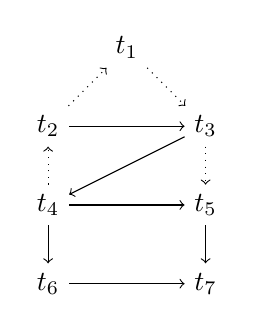
\begin{tikzpicture}
\node at (0,3) (alpha) {$t_1$};
\node at (-1,2) (beta)  {$t_2$};
\node at (1,2) (gamma)  {$t_3$};
\node at (-1,1) (delta)  {$t_4$};
\node at (1,1) (epsilon)  {$t_5$};
\node at (-1,0) (zeta)  {$t_6$};
\node at (1,0) (eta)  {$t_7$};

\draw[dotted, ->] (beta)->(alpha);
\draw[dotted, ->] (alpha)->(gamma);
\draw[->] (beta)->(gamma);
\draw[dotted, ->] (delta)->(beta);
\draw[->] (delta)->(epsilon);
\draw[->] (gamma)->(delta);
\draw[->] (epsilon)->(eta);
\draw[dotted, ->] (gamma)->(epsilon);
\draw[->] (zeta)->(eta);
\draw[->] (delta)->(zeta);

\end{tikzpicture}
\end{minipage}
\caption{Two graphs $G_1$ and $G_2$. $G_1$ is (node disjoint) subgraph homeomorphic to $G_2$ with the mapping $\{(s_1, t_5), (s_2, t_7), (s_3, t_4), (s_4, t_2), (s_1 \to s_2, t_5 \to t_7), (s_3 \to s_1, t_4 \to t_5), (s_3 \to s_2, t_4 \to t_6 \to t_7), (s_4 \to s_3, t_2 \to t_3 \to t_4)\}$. Other homeomorphisms exist as well.}
\end{figure}

If we have graphs $G_{virtual}$ and $G_{concrete}$, then wherever a subgraph homeomorphism from $G_{virtual}$ to $G_{concrete}$ exists, it describes a mapping where the logic of the virtual FPGA may be performed on the concrete FPGA in an emulation\footnote{If no such relation exists, it does not mean a function $f$ as specified in Section \ref{sec:Objectives} does not exist. Emulation could still be obtained by emulation of components by (multiple) components of possibly different types or by emulation of routing switches by sets of connected routing switches.}\footnote{This does not hold if some vertices in $G_{concrete}$ that are part of the mapping are unconfigurably connected and their mapped equivalents in $G_{virtual}$ are not. This is, however, rare and we account for this in our algorithm.}. The vertex-to-vertex mapping $\mathit{vmap}$ describes how to obtain configurations for the concrete FPGA and the edge-to-path mapping $\mathit{emap}$ describes how vertices in the concrete FPGA are connected via paths of intermediate components configured as wires.


The similarity between \textit{subgraph isomorphism} and \textit{subgraph homeomorphism} allows us to take inspiration from existing subgraph isomorphism algorithms and use similar methods to solve subgraph homeomorphism and therewith the FPGA emulation problem.



\chapter{Objectives}
\label{sec:Objectives}
This research involves how to emulate a virtual FPGA on a concrete FPGA. To this purpose, we have established the following research question:

Given a graph specification of the structural layout of a virtual FPGA $A$ and a graph specification of the structural layout of a concrete FPGA $B$, how do you assemble a linear\footnote{i.e. a numeric constant $c$ exist such that the number of instructions required in the execution of $f$ is less than $c * (\text{the number of configurable components of the virtual FPGA})$. Note that this depends on the size of the \textit{unconfigured} virtual FPGA, not on the size of the user-provided configuration of said FPGA.} function $f$ such that for any representative model of a program $x$ for model A, $f(x)$ is a representative model of a program for model B that is semantically equivalent?
\section*{Subquestion 1}
How do the computational- and space requirements of the generation (not execution) of $f$ scale with the size of FPGAs A and B?
\section*{Subquestion 2}
How much wiring and how many components does the concrete FPGA need for emulation of a virtual FPGA of complexity $x$? Is this practical for use in education?
\section*{Expected outcomes}
We expect an algorithm and an implementation of that algorithm that, given models of both a virtual FPGA and a (larger) concrete FPGA, generates a function that translates a model of an FPGA program compatible with the virtual FPGA to a model of an FPGA program compatible with the concrete FPGA. We generalise this algorithm to other use cases with the same underlying mathematical problem (node disjoint subgraph homeomorphism). Furthermore, we include specifications on how to model FPGA models for this purpose. 
\chapter{Models}
Our algorithm will generate an emulation using vertex disjoint subgraph homeomorphism. For this purpose, we will use vertex-multilabeled directed simple graphs as defined in Definition \ref{def:graph}. In these graphs we will:

\begin{itemize}
\item ..model a wire as a vertex that may be connected with any number of vertices in either direction of types ``$arc$", any number of incoming edges from ``$port\_out$" vertices and any number of outgoing edges to ``$port\_in$" edges.
\item ..model a transistor as a vertex with a label ``$arc$" and a label ``$configurable$" for configurable transistors or label ``$unconfigurable$" for unconfigurable transistors (that are not counted towards label compatibility). It has an incoming edge from the source ``$wire$" of the transistor and an outgoing edge to the target ``$wire$" of the transistor.
\item ..model a LUT as a vertex with label $``lut"$ that only has connections from vertices with label ``$port\_in$" and to vertices with label ``$port\_out$".
\item ..model a register as a vertex with label ``$register$" that only has connections from vertices with label ``$port\_in$" and to vertices with label ``$port\_out$"..
\item ..model an input of a component as a vertex with label ``$port\_in$" and an outgoing directed edge towards a ``$lut$" or ``$register$" vertex and an incoming edge from a ``$wire$" vertex.
\item ..model an output of a component as a vertex with label ``$port\_out$" and an incoming directed edge from a ``$lut$" or ``$register$" vertex and an outgoing edge to a ``$wire$" vertex.
\end{itemize}

An example of such am model is shown in Figure \ref{fig:graphmodel-logiccell} where a graph model is shown of the logic cell in Figure \ref{fig:logiccell}.

\begin{figure}
\includegraphics[width=\textwidth]{images/modelOfCell.png}
\caption{Graph model of the logic cell shown in Figure \ref{fig:logiccell}}
\label{fig:graphmodel-logiccell}
\end{figure}

\chapter{Algorithm}

\tikzstyle{decision} = [diamond, align=center, draw=black]

\tikzstyle{block} = [rectangle, minimum width=2.5cm, minimum height=1cm, align=left, draw=black]


\section{Baseline: ndSHD2}
In our research we will extend existing work on node disjoint subgraph isomorphism. In the literature we found two existing well-defined algorithms: Xiao's algorithm `ndSHD2' \cite{XIAONODEDISJOINT} and Lingas algorithm \cite{LINGAS2009464}. We choose to adapt Xiao's algorithm ndSHD2 as baseline over Lingas because it is simpler, includes a method for calculating a vertex-on-vertex mapping and has many similarities with subgraph isomorphism algorithms. In comparison, Lingas' algorithm suggests attempting their edge-path mapping strategy on every possible vertex-on-vertex mapping. We will adapt Xiao's algorithm to compute paths on-the-fly instead of beforehand to avoid the exponential space requirement.

To understand ndSHD2 better, let us first examine what the output is supposed to be. The algorithm should, given two graphs, not just indicate whether the latter graph has a subgraph homeomorphism of the former, but also indicate what subgraph homeomorphism that is. More formally, we need to solve the \textit{certification} problem rather than the \textit{decision} problem. This certification indicates to which target graph vertex each source graph vertex is mapped and to which target graph path each source graph edge is mapped such that the entire mapped source graph is a subgraph of the target graph. This is what we will from now on refer to as the \textbf{mapping}. If, during the execution, the mapping is not yet complete, i.e. it does not have a target for some source graph vertex or edge, we refer to it as the \textbf{partial mapping}.

\begin{algorithm}
\SetAlgoLined
\textbf{Inputs: } the current vertex-vertex partial mapping $\mathit{vmap}$, the current edge-path $\mathit{emap}$ partial mapping\\
\textbf{Outputs: } \textit{found}, indicating whether a valid subgraph homeomorphism has been found.\\
\If{$s$ is dead state} {
	\Return false\;
} \ElseIf {$s$ is complete} {
	\Return true\;
}

$\mathit{found} \longleftarrow \mathit{false}$

 \While{$!\mathit{found} \land \exists$ valid node/edge-path mapping pair}{
  $m \longleftarrow \mathit{GetNextNodePair}()$\tcp*[h]{$m \longleftarrow \mathit{GetNextEdgePathPair}()$}\;
  
  \If{$\mathit{wouldPrune}(\mathit{vmap}, \mathit{emap}, m)$} {
  	\textbf{continue}\;
  }  
  
  $\mathit{vmap}' \longleftarrow \mathit{Backup}(\mathit{vmap})$\tcp*[h]{ 
  $\mathit{emap}' \longleftarrow \mathit{Backup}(\mathit{emap})$}\; 
  $\mathit{vmap} \longleftarrow \mathit{vmap} \cup \{m\}$\tcp*[h]{$\mathit{emap} \longleftarrow \mathit{emap} \cup \{m\}$}\;  
  
  $\mathit{found} \longleftarrow \mathit{ndSHD2}(s, \mathit{vmap}, \mathit{emap})$\;
  \If{found} {
  	\Return true\;
  }
  $\mathit{vmap} \longleftarrow \mathit{Recover}(\mathit{vmap})$\tcp*[h]{ 
  $\mathit{emap}' \longleftarrow \mathit{Recover}(\mathit{emap})$}\;
 }
 \Return false\;
 \caption{ndSHD2}
 \label{algorithm:ndSHD2}
\end{algorithm}


\begin{algorithm}
\SetAlgoLined
\textbf{Inputs: } the current vertex-vertex partial mapping $\mathit{vmap}$, the current edge-path $\mathit{emap}$ partial mapping\\
\textbf{Outputs: } \textit{found}, indicating whether a valid subgraph homeomorphism has been found.\\

\If{contraction} {
	$G_S, \mathit{chains} \longleftarrow \mathit{contract}(G_S)$
}

 \Return ndSHD3($\mathit{vmap}$, $\mathit{emap}$)\;
 \caption{ndSHD3-contract}
 \label{algorithm:ndSHD3}
\end{algorithm}

\begin{algorithm}
\SetAlgoLined
\textbf{Inputs: } the current vertex-vertex partial mapping $\mathit{vmap}$, the current edge-path $\mathit{emap}$ partial mapping\\
\textbf{Outputs: } \textit{found}, indicating whether a valid subgraph homeomorphism has been found.\\

\If {$s$ is complete} {
	\Return true\;
}

$\mathit{found} \longleftarrow \mathit{false}$

 \While{$!\mathit{found} \land \exists$ valid node/edge-path mapping pair}{

\If{$\mathit{hasUnmatchedEdge}()$} {
	$(e_S, p_T) \longleftarrow \mathit{GetNextEdgePathPair}()$\;
	\If{$\mathit{wouldPrune}(\mathit{vmap}, \mathit{emap} \cup \{(e_S, p_T)\})$} {
  		\textbf{continue}\;
  	}
  	$\mathit{emap} \longleftarrow \mathit{emap} \cup \{(e_S, p_T)\}$\;
  	$\mathit{found} \longleftarrow \mathit{ndSHD3}(\mathit{vmap}, \mathit{emap})$\;
  \If{found} {
  	\Return true\;
  }
  $\mathit{emap} \longleftarrow \mathit{emap} \cap \{(e_S, p_T)\}$\;
} \Else {
	$(v_S, v_T) \longleftarrow \mathit{GetNextNodePair}()$\;
	\If{$\mathit{wouldPrune}(\mathit{vmap} \cup \{(v_S, v_T)\}, \mathit{emap})$} {
  		\textbf{continue}\;
  	}
  	$\mathit{vmap} \longleftarrow \mathit{vmap} \cup \{(v_S, v_T)\}$\;
  	$\mathit{found} \longleftarrow \mathit{ndSHD3}(\mathit{vmap}, \mathit{emap})$\;
  \If{found} {
  	\Return true\;
  }
  	$\mathit{vmap} \longleftarrow \mathit{vmap} \cap \{(v_S, v_T)\}$\;
}

 }
 \Return false\;
 \caption{ndSHD3}
 \label{algorithm:ndSHD3}
\end{algorithm}




\begin{algorithm}
\SetAlgoLined
\textbf{Inputs: } the current vertex-vertex partial mapping $\mathit{vmap}$, the current edge-path $\mathit{emap}$ partial mapping\\
\textbf{Outputs: } whether pruning should be applied.\\
$\mathit{domains} \longleftarrow \mathit{filterDomains}(\mathit{vmap}, \mathit{emap})$\;
\If {ZeroDomain} {
	\If {$\emptyset \in \mathit{values}(\mathit{domains})$} {
		\Return false\;
	}
} \ElseIf {AllDifferent} {
	\If {$\lnot \mathit{satisfiesAllDifferent}(\mathit{domains})$} {
		\Return false\;
	}
}
\Return true\;
 \caption{wouldPrune}
 \label{algorithm:ndSHD3}
\end{algorithm}


ndSHD2 Is shown in Algorithm \ref{algorithm:ndSHD2}. It is a form of depth first search in a partial mapping search space that attempts- and backtracks vertex-on-vertex mappings and edge-on-path mappings.

In our literature study, we found that the core of many subgraph isomorphism algorithms\footnote{Ullman, VF, VF2, VF2+, VF2++, UI, Fast-ON, L2G, Cheng, QuickSI, GraphQL, ILF, TurboISO, Glassgow, CLF-Match, RI, RI-DS, McGregor, LAD, PathLAD} is a form of similar DFS state space exploration where the states consist of partial vertex-to-vertex mappings. In subgraph isomorphisms, the edge-to-edge mapping is elementary by performing the vertex mapping on the edge source and target to obtain the target edge. With the subgraph homeomorphism algorithm such as Xiao's, an additional mapping from $E_S$ to the path set of $G_T$ is needed.

The algorithm starts with an empty partial mapping, and starts mapping source graph vertices to target graph vertices. Whenever both vertices of a source graph edge have been matched, the algorithm finds an arbitrary path between the mapped edge source and target in the target graph that is internally disjoint from target graph vertices already used in the partial mapping. The algorithm prioritizes extending the matching with an edge-path pair over extending it with a vertex-vertex pair. Whenever no such path or vertex exists, the algorithm undoes (backtracks) the last matching step taken and tries a different alternative. Whenever a partial match is extended with a vertex-vertex pair or with an edge-path pair the search space is refined using a pruning strategy implemented by the $Refine(M,R)$ call. This method filters out future path candidates from a path storage and from a vertex storage according to zero-domain N-reachability pruning (see Chapter \ref{chapter:pruning} for definitions). This removes path candidates and vertex candidates that can provably not be part of any valid subgraph homeomorphism mapping.

The algorithm as specified in Xiao's paper leaves out some specific ordering details- we will assume that they used random ordering. We specify which vertex order we use in Sections \ref{sec:sourceOrder}, \ref{sec:targetOrder}. We will explain what order of paths we use in Section \ref{sec:pathIterationShort}.

\section{How to choose vertex-vertex pairs}
There are different ways to choose which vertex-vertex pair to add to the partial mapping first, and which only to try after other attempts have failed. These methods can be divided into three categories:

\begin{enumerate}
\item Choose a source graph vertex first using some heuristic, then attempt all target graph vertex candidates using another heuristic.
\item Choose a target graph vertex first using some heuristic, then attempt all source graph vertex candidates using another heuristic.
\item Choose a source vertex-target vertex with high heuristic first, then attempt all other pairs.
\end{enumerate}

While the strategy used does not affect the vertex-on-vertex mapping state space, it can affect the average-case performance. Strategy 3, for example, uses combined heurstics that may be more powerful. The disadvantage of it requires $O(|V_s|*|V_t|)$ heuristic computations before the first pair is obtained. If these computations are done beforehand the heuristic cannot take the current partial mapping into account and is likely to be weak. Is this computation is done at each step in the search process, it introduces considerable delay.

Strategies 1 and 2, on the other hand, require only $O(|V_s|+|V_t|)$ heuristic calculations to be made before obtaining a candidate pair. We choose a source graph vertex heuristic that is precomputed and provide two heuristics for target graph vertices, one of which is precomputed and one of which is calculated run-time.

\section{Source graph vertex order}
\label{sec:sourceOrder}
The source graph vertex order is the order in which source graph vertices are added to the partial mapping. For example, if $s_1 \prec_M s_2$ in this ordering, then a pair with $s_2$ and some target graph vertex will only be added to the partial mapping if a pair with $s_1$ is already in it within the context of a partial matching $M$. If this ordering depends on $M$, it has to be calculated at run-time. If it does not, it only has to be calculated once.

Xiao does not specify a source graph vertex order. Instead, we will use a high-performance ordering technique from the subgraph \textit{isomorphism} domain. From performance comparisons we extract that the best performing algorithm that adheres to partial mapping search for subgraph isomorphism is RI-DS. In our literature study, we found no evidence a faster algorithm exists. This ordering does not depend on $M$, and thus we will precompute the entire ordering.

To describe the ordering process of RI-DS, let us provide a few definitions:

\begin{defn}[predecessors and successors]
Given two graphs $G=(V, E, L)$ and some vertex $v \in V$, their predecessors and successors are defined as follows:

$\mathit{succ}(v) := {v' \in V . (v, v') \in E}$

$\mathit{pred}(v) := {v' \in V . (v', v) \in E}$
 
\end{defn}

\begin{defn}[neighbour set]
If some $v\in V$, then $\mathit{neighbours}(v):= \mathit{succ}(v) \cup \mathit{pred}(v)$.
\end{defn}

%\begin{defn}[E for sets of vertices]
%If some $S\subseteq V$, then $E(S):=\bigcup\limits_{v \in S} E(v)$.
%\end{defn}


The algorithm RI-DS obtains a variable ordering using a greedy algorithm called ``GreatestConstrainedFirst". This algorithm starts with an ordering $\mu$ containing only the source graph vertex with the highest degree, i.e. $v\in V_1$ where $|\mathit{neighbours}(v)|$ is highest. Then, each source graph vertex not yet in the order is assigned three scores $N_1$, $N_2$ and $N_3$. $N_1(s_x)$ is the number of neighbours of $s_x$ that are already in the order (i.e. $|\{s_y | s_y \in \mathit{neighbours}(s_x) \land s_y \in \mu\}$|). $N_2(s_x)$ is the number of neighbours of $s_x$ that are not in the order themselves, but do have a neighbour in the order (i.e. $|\{s_y | s_y \in \mathit{neighbours}(s_x) \land s_y \not \in \mu \land |\mathit{neighbours}(s_y) \cap \mu| > 0\}$|). $N_3(s_x)$ is the number of all remaining neighbours of $s_x$ (i.e. $|\{s_y | s_y \in \mathit{neighbours}(s_x) \land s_y \not \in \mu \land |\mathit{neighbours}(s_y) \cap \mu| = 0\}$|). It selects each vertex $v$ of which $N_1(v)$ is greatest. Ties are broken with the greatest $N_2$-value, and any remaining ties are broken with the greatest $N_3$-value. Any remaining ties are broken randomly. The selected vertex is added to the back of the order, and the process repeats. This continues until every vertex has been added to the order.

The result of this ordering is that consequent vertices have many edges with vertices earlier in the ordering. Xiao established that matching edges as soon as possible (rather than matching vertices first) results in a faster algorithm. Using an order that allows early placement of edges such as GreatestConstrainedFirst should accoring to Xiao result in fast execution.
\section{Target graph vertex order}
\label{sec:targetOrder}

The target graph vertex order is the order in which target graph vertices are added to the partial mapping. For example, if $t_1 \prec t_2$ in this ordering, then a pair with $t_2$ and some source graph vertex $s_x$ will only be added to the partial mapping if the pair $(s_x, t_1)$ was already proved unfeasible. Xiao does not describe a specific target graph vertex order.

We found one subgraph isomorphism algorithm that describes a specific target graph vertex order, being Glasgow \cite{McCreesh2015}. In this algorithm, target graph vertices with higher degree are prioritized. Since this does not depend on the chosen source graph vertex or on the current partial matching, this order can be precomputed, introducing only linear complexity. Formally, when some source graph vertex $s$ needs to be matched, $x$ are chosen using the following metric, choosing vertices with lower metric values first:

$$\mathit{metric}_\mathit{degree}(s, t)=-|\mathit{neighbours}(t)|$$

Another option is to take the current partial mapping into account. Using a degree-based or random target graph vertex order will result in consectively chosen target graph vertices being spread roughly evenly throughout graph. Since we optimise our algorithm for large target graphs, chosen vertices at arbitrary locations will likely result in long paths necessary to reach them, and thus in unneccessary resource usage. However, we can use information from the current partial mapping to obtain better candidates: since we know the chosen source graph vertex and thus which edges will be mapped after this vertex-vertex pair, we can choose our target vertex such that the paths associated with these edges are as short as possible.

Whenever we need to match some source graph vertex $s_x$, This distance-based method will choose target vertices first that have the lowest distance to the source graph vertex' neighbours that are already in the partial matching. The result is that fewer number of vertices need to be used as intermediate vertex in the paths associated with the edges to those neighbours. The disadvantage of this method is that it requires runtime usage of a computionally expensive shortest path algorithm to choose a target graph vertex candidate. The shortest path algorithm can be cached, which reduces the number of computations needed after backtracking but introduces quadratic\footnote{$O(|V_s|*|V_t|)$} space usage (we implement this with- and without caching). Formally, when some source graph vertex $s_x$ needs to be matched, $t_x$ are chosen using the following metric, choosing vertices with lower metric values first:


$$\mathit{metric}_\mathit{distance}(s, t)=\sum_{s' \in E(s)} \begin{cases}
|\mathit{shortestPathUndirected}(M(s'), t)| & s' \prec_\mu s\\
0 & s \prec_\mu s'
\end{cases}$$

Here, $M$ is the current partial mapping and $\mu$ is the source graph vertex order. We implemented both methods to use in our algorithm.

\section{Path iteration}
\label{sec:pathIterationShort}
In subgraph isomorphism, edge-on-edge mappings are trivial from vertex-on-vertex mappings. However, in subgraph homeomorphism a source graph edge may be mapped on many target graph path candidates (all starting- and ending at the same two vertices). Therefore, we cannot extract the order in which to try out paths from subgraph isomorphism. Instead, we implemented different methods to iterate over paths to try:

\begin{itemize}
\item \textbf{K-path -} Try all loopless paths from shortest to longest, avoiding unusable vertices in the existing partial mapping. We use Yen's algorithm \cite{YensAlgorithm} for this. Faster and more recent algorithms exist \cite{Hershberger, Brander1996} but lack public implementations.

\item \textbf{DFS -} Search for paths using depth first search from the start vertex, choosing arbitrary directions at each vertex and avoiding unusable vertices in the existing partial mapping.

\item \textbf{Greedy DFS (graph distance) -} Search for paths using greedy depth first search, choosing the direction closest to the goal vertex first (avoiding unusable vertices in the existing partial mapping). We implement both a variant that precomputes all shortest paths and a variant that calculates at run-time which direction to choose (without caching).

\item \textbf{Greedy DFS (informed graph distance) -} Search for paths using greedy depth first search, choosing the direction closest to the goal vertex along a path that avoids unusuble vertices first (avoiding unusable vertices in the existing partial mapping). We compute run-time which direction to choose.

\item \textbf{Control point -} Select increasingly many `control points' (from $0$ to $|V|$) randomly in the target graph that must be in the path in a specific order, then connecting them by a shortest path algorithm that avoids unusable vertices in the existing partial mapping. We implemented this with a recursive algorithm in which a replacement of some control point is only attempted if all control points \textit{earlier} in the control point order have been attempted.\footnote{To avoid duplicate paths, any path that can be generated with fewer control points is skipped. Furthermore, any control point configuration where shifting some control point towards the goal vertex along the path results in the same path is skipped.}
\end{itemize}

These methods provide for each two vertices in a graph each path connecting them exactly once. The space requirements for each method are shown in Table \ref{tab:iterator-spacerequirements}, and examples of paths returned by them are shown in Appendix 2.

\begin{table}[]
\centering
\begin{tabular}{|l|l|}
\hline
\textbf{Path iterator} & \textbf{Space complexity} \\ \hline
K-Path                 & $O(|V|!)$                 \\ \hline
DFS                    & $O(|V|)$                  \\ \hline
Greedy DFS             & $O(|V|^2)$                \\ \hline
Control point          & $O(|V|)$                  \\ \hline
\end{tabular}
\caption{Worst-case space complexity of each path iteration strategy. The computational requirements of each method change in different ways for subsequent calls.}
\label{tab:iterator-spacerequirements}
\end{table}


\section{Optimisations}
In addition to implementing ordering parameters of the ndSHD2 algorithm, we implement some optimisations (some of which from the subgraph isomorphism domain) and individually evaluate them. 

\subsection{Refusing long paths}
Since path iterators may provide any valid path to map an edge to during the matching process, they may also provide paths that take up unnecessarily many resources. Specifically, they take up so many resources that with a subset of the vertices and edges of that path, a shorter path can be formed. Formally, some path $p$ is ``unnecessarily long" iff:


$\exists p' \in P . first(p') = first(p) \land last(p') = last(p) \land intermediate(p') \subset intermediate(p)$

With this optimisation enabled, such paths are skipped by path iterators. Examples of this effect are shown in Figures \ref{fig:pathexamples-dfs} and \ref{fig:pathexamples-greedydfs}.

\subsection{Runtime Pruning}
Some subgraph isomorphism algorithms \cite{Cordella2004, McCreesh2015} prune the search space during the search using some detection method of dead search paths. In Chapter \ref{chapter:pruning} we will elaborate on the different techniques we implement for subgraph homeomorphism.

\subsection{Contraction}
The source graph of a homeomorphism case will often contain vertices that have exactly one incoming edge and one outgoing edge. In FPGAs, for example, these could be transistors or ports of components. These vertices do topologically nothing but serve as an edge; therefore they may also be thought of as an edge, where the edge source is the vertex' predecessor and the edge target is the vertex' successor. When we use the word contraction, we mean surpressing all such vertices and replacing them with a single edge, as illustrated in Figure \ref{fig:contraction-basic}. This process transforms the source graph $S$ into the smallest graph $S_{cont}$ that is topologically equivalent to $S$. This may be a multigraph or a graph that contains self-loops. If a subgraph homeomorphism exists from $S$ to some target graph $T$, then there also exists a subgraph homeomorphism from $S_{cont}$ to $T$ (a proof is given in Appendix \ref{proof:contractionHomeo}). The optimisation `contraction' searches for a homeomorphism between $S_{cont}$ and the $T$ instead of finding one between $S$ and $T$. Because this involves a smaller source graph, it also involves a smaller search space.

The process of finding a homeomorphism from $S_{cont}$ to $T$ is slightly different from what normal. This is because while every homeomorphism from $S$ to $T$ can be deduced to a homeomorphism between $S_{cont}$ and $T$ (by contraction of vertices and concatenation of paths), not every homeomorphism from $S_{cont}$ and $T$ allow a homeomorphism from $S$ to $T$ to be inferred. An example is the case where $S_{cont}$ is isomorphic to $T$ and $S$ subdivides a single edge of $S_{cont}$: there exists a subgraph homeomorphism from $S_{cont}$ to $T$ since they are isomorphic, but there is no subgraph homeomorphism from $S$ to $T$. Because of this, we need to adapt the subgraph homeomorphism search process such that it only finds subgraph homeomorphisms from which we \textit{can} infer a subgraph homeomorphism from $S$ to $T$.

When we apply contraction to replace a series of edges $E$ by a single edge $e$, we save the label sets for each intermediate vertex in $E$ in the order that they appear (following the direction of $e$) before starting the search algorithm. 

During edge-path matching in the partial mapping search, we may need to map an edge $(u, v)$ that contains contracted vertices. For each edge $\in E_{cont}$ with the same source- and target vertex we recall their lists of contracted label sets. Each time we find a path candidate for $(u, v)$ we check compatibility of that path with each of those lists of label sets. We then retrieve all other paths already found for edges with this source- and target and use an all-different constraint (see Section \ref{sec:alldifferent}) to verify that each edge $\in E_{cont}$ has a compatible path. Whenever the number of paths is smaller than the number of edges (i.e. paths still need to be found futher in the partial mapping search), we assume paths that are compatible with every list of label sets.

If the all-different constraint fails, it implies that from the current partial mapping we cannot find paths that emulate the contracted vertices, and we backtrack. If the all-different constraint succeeds, finding a subgraph homeomorphism is still possible and we continue.

This optimisation introduces some delay since the algorithm needs to check compatibility between label set sequences and paths and solve an all-different constraint. However, it also saves time since it reduces the source graph's size.

\subsubsection{Contraction for undirected graphs}
Although we are focued on directed graphs in our algorithm, it is interesting to note that each optimisation is also applicable to undirected graphs, including contraction. Contraction can be applied to undirected graphs by temporarily applying a uniform direction to each chain of 2-degree vertices in the source graph and then applying directed contraction, after which the edges may lose their direction again. Then, during the compatibility checking process we perform the same procedure, making sure the list of label sets is checked in the correct direction, i.e. for each temporarily directed edge $(u, v) \in E_{cont}$ and partial mapping $M$, the path $M(u, v)$ in $T$ should be checked in the direction from $M(u)$ to $M(v)$.



\begin{figure}
\begin{subfigure}{.5\textwidth}
  \centering
\includegraphics[width=0.8\linewidth]{images/contraction/whatisit1.png}
  \caption{Part of a source graph that may be contracted}
\end{subfigure}
\begin{subfigure}{.5\textwidth}
  \centering
\includegraphics[width=0.8\linewidth]{images/contraction/whatisit2.png}
  \caption{The result of contraction}
\end{subfigure}
\caption{Contraction applied to vertex $s_2$, a vertex with indegree 1 and outdegree 1. During contraction, we save that a single vertex has been contracted with an empty label set.}
\label{fig:contraction-basic}
\end{figure}


\begin{figure}
\begin{subfigure}{.5\textwidth}
  \centering
\includegraphics[scale=0.6]{images/contraction/after.png}
  \caption{A source graph before contraction}
\end{subfigure}
\begin{subfigure}{.5\textwidth}
  \centering
  % include second image
\includegraphics[scale=0.6]{images/contraction/before.png}
  \caption{The same source graph after contraction.}
\end{subfigure}
\caption{Contraction applied to a source graph with labels. With this optimisation, 3 fewer vertices and 4 fewer edges need to be mapped. During contraction, we save the label sets of the contracted vertices in the order of the contracted path.}
\label{fig:contraction}
\end{figure}


\section{Avoiding unintended current flow}
\label{sec:unintendedcurrent}
As mentioned in Chapter \ref{chapter:models}, the concrete FPGA may contain transistors that are always enabled, i.e. cannot be configured to block the flow of electrical current and function as a diode. If we would ignore this property of transistors, we may obtain a mathematically sound subgraph homeomorphism that does not include every unconfigurable transistor from the target graph in its mappings. If some unconfigurable transistor (or a sequence of them) connect two vertices in the target graph that \textbf{are} part of the mapping, then the subgraph homeomorphism does not describe a valid emulation: if the state of two components are independent in the virtual FPGA they should be independent in the concrete FPGA as well to preserve the semantics of the FPGA configuration. To avoid this issue, we propose two measures:

\subsection{Avoiding unintended current flow from/to paths}
Our first remedy is to avoid adding target graph vertices to the partial mapping that are connected to some path already present in the edge-path partial mapping through unconfigurable vertices. We do this by deleting those vertices and re-adding them whenever we backtrack the corresponding edge-path pair. More formally:

Let $\mathit{unconfigurable}\in (V_T \times V_T)$ be the relation between two vertices if they are connected through a vertex representing a unconfigurable transistor, i.e:

\vspace{10pt}

\begin{center}
\begin{tabular}{ll}
$\mathit{unconfigurable} := \{(t_1, t_2) \in (V_T \times V_T) | \exists u \in (V_T \setminus \{t_1, t_2\}) .$&$\mathtt{UNCONFIGURABLE} \in L(u) \land$\\
&$\{(t_1, u), (u, t_2)\} \subseteq E_T\}$
\end{tabular}
\end{center}

\vspace{10pt}
Let $\mathit{unconfigurable}^*$ be the symmetric closure of the transitive closure of $\mathit{unconfigurable}$. Then, whenenever we add an edge-path pair $(e, p)$ to the partial mapping, we delete each vertex $x$ for which $\exists v \in \mathit{intermediate}(p) . (x, v) \in \mathit{unconfigurable}^*$. Whenever the edge-path pair is removed from the partial mapping, each such vertex and their edges is added back to the target graph.


\subsection{Avoiding unintended current flow between mapped vertices}
Our second remedy is to avoid adding target graph vertices to the partial mapping that are connected to some target graph vertex already present in the vertex-vertex partial mapping through unconfigurable vertices. We also do this by deleting those vertices and re-adding them whenever we backtrack the corresponding vertex-vertex pair. More formally, whenever we add a vertex-vertex pair $(s, t)$ to the partial mapping, we delete each vertex $x$ for which $(x, t) \in \mathit{unconfigurable}^*$. Whenever the vertex-vertex pair is removed from the partial mapping, each such vertex and their edges is added back to the target graph.






\chapter{Pruning}
\label{chapter:pruning}

During the search for a complete matching, during which the algorithm only has \textit{partial} matchings, the algorithm will often explore branches of the search tree that will not eventually lead to a homeomorphism. We will call these branches \textit{dead branches}. Exploring an entire dead branch may be costly: its size is exponential\footnote{due to the NP-completeness of node disjoint subgraph homeomorphism} thus exploration costs an exponential amount of time. A solution to this is to implement methods of early detection of such dead branches, i.e. pruning methods. These methods can by nature not detect every dead branch efficiently\footnote{again, because of the NP-completeness of node disjoint subgraph homeomorphism.}. Therefore, there exists a tradeoff between strength, i.e. how many dead branches it can detect, and performance, i.e. how the number of instructions used by pruning scales with the size of the inputs. Xiao's algorithm uses various pruning methods, which we will implement for our algorithm. We implement these algorithms without precomputed paths, i.e. we run a pathfinding algorithm during the partial mapping search instead and optionally cache the results.

The input of these pruning methods comes down to an assignment of domains (sets of target graph vertices) to variables (source graph vertices). These domains represent the target graph vertex candidates for each source graph vertex in vertex-on-vertex matching. Source graph vertices that are already in the partial matching have a domain of size one: the target graph vertex they have been matched to. The other vertices have domains that can be calculated in different ways (see Section \ref{sec:domain-filtering}). The pruning method then decides whether the algorithm should continue the search in this branch (i.e. do not prune) or whether the algorithm should backtrack. The different methods of deciding this are elaborated in Section \ref{sec:pruningmethods}.

\section{Domain filtering}
\label{sec:domain-filtering}
The goal of domain filtering during a search is to assign a domain of target graph vertices to each source graph vertex such that the following three criteria are satisfied:

\begin{enumerate}
\item \label{li:complete}If at least one homeomorphism can be found from this search branch, then for some homeomorphism that can be found from this search branch with vertex-on-vertex matching $M_V$ it holds that $\forall (s \to t) \in M_V . t \in \mathit{domain}(s)$.
\item \label{li:falsepositives}Each domain assignment contains as few `false positives' as possible, where a false positive is a pair of a source vertex $s$ and a target vertex $t$ such that $t$ is in the domain of variable $s$ and no homeomorphism exists from the current search path in which $s$ is matched to $t$.
\item \label{li:complexity} The process of domain filtering has a computational complexity that is as low as possible.
\end{enumerate}

In this section, we will explore different methods to obtain these domains, each with different tradeoffs between strength (performing better at criterium \ref{li:falsepositives}) and performance (performing better at criterium \ref{li:complexity}). While technically any combination of these methods can be in combination (i.e. by intersecting the domains they find), we limit ourselves with the assumption that each method is combined with every computationally cheaper filtering method.
\subsection{Labels and neighbours}
The weakest and fastest method to obtain domains for some source graph vertex $u$ is by selecting each target graph vertex $v$ that is not already used in the current partial mapping, has compatible labels and has compatible in- and outdegrees:

\begin{minipage}{\textwidth}
\begin{defn}[compability under label constraint] If $M$ is the current partial matching, then:

\begin{center}
\bgroup
\def\arraystretch{1.2}
\setlength\tabcolsep{5pt}
\begin{tabular}{lll}
\centering
$\mathit{compatible}_{\mathit{LABEL}}(s,t) := $&$t \not \in M$&$\land$\\
&$L(s) \subseteq L(t)$&$\land$\\
&$|\mathit{pred}(t)| \geq |\mathit{pred}(s)|$&$\land$\\
&$|\mathit{succ}(t)| \geq |\mathit{succ}(s)|$&\\
\end{tabular}
\egroup
\end{center}

\end{defn}
\end{minipage}

This method satisfies criterium 1 since every homeomorphism needs each source graph vertex $s$ to be matched with a target graph vertex $t$ that has at least the same label set as $s$, and the possibility of connecting with each mapped predecessor and successor of $s$. It has a low computational complexity per source-target pair ($O(|L_S|)$).

\subsection{Free neighbours}
A somewhat stronger and somewhat slower method to obtain domains in addition to label filtering is to compare the indegree- and outdegree of each unmatched source graph vertex $s$ to other unmatched source graph vertices to the in- and outdegree of the target graph vertex $t$ to other unmatched target graph vertices. The target graph vertex must have a larger or equal indegree and outdegree compared to the source graph vertex:


\begin{minipage}{\textwidth}
\begin{defn}[compatibility under free neighbours constraint] If $M$ is the current partial matching, then:


\begin{center}
\bgroup
\def\arraystretch{1.2}
\setlength\tabcolsep{5pt}
\begin{tabular}{lll}
\centering
$\mathit{compatible}_{\mathit{FN}}(s,t) := $&$\mathit{compatible}_{\mathit{LABEL}}(s,t)$&$\land$\\
&$ |\mathit{pred}(t) \setminus M| \geq |\mathit{pred}(s) \setminus M|$&$\land$\\
&$ |\mathit{succ}(t) \setminus M| \geq |\mathit{succ}(s) \setminus M|$
\end{tabular}
\egroup
\end{center}
 
\end{defn}
\end{minipage}

This method satisfies criterium \ref{li:complete} since each unmatched neighbour must yet be matched with a target graph vertex that is (vertex disjointly) connected with the target graph vertex. For this purpose, unused connection to the vertex are required. It has a slightly higher computational complexity per source-target pair ($O(|L_S| + |E_S|/|V_S| + |E_T|/|V_T|)$)


\subsection{Reachability of matched vertices (M-filtering)}
A strong (and computationally very expensive) method of filtering the domain we will use for some source graph vertex $s$ and some target graph vertex $v$ in addition to label- indegree and outdegree compability is to check that $v$ can reach the mapped vertices of successors of $s$ and that $v$ can be reached from the mapped vertices of predecessors of $s$, i.e. that candidate paths exist for the upcoming edge-path matching attempts. This pruning method does not check whether a set of paths exist that is vertex disjoint since that is the task of the main algorithm: it merely checks the existence of paths. If no path exists, then no vertex disjoint path exists and pruning is required. An example of a domain filtered by reachability can be found in Figure \ref{fig:reachability-filtered}. Formally:
%An even stronger method would be to find paths that each have different second vertices and each have different second-last vertices, or even to check that no intermediate vertex is used multiple times (NP-complete). This is, however, out of scope for this research.

\begin{minipage}{\textwidth}
\begin{defn}[compatibility under reachability constraint]

If $M$ is the current partial mapping and $P$ is the set of paths in the target graph, then:

\bgroup
\def\arraystretch{1.5}
\setlength\tabcolsep{0pt}
\begin{tabular}{lll}
\centering
$\mathit{compatible}_{\mathit{M-REACH}}(s,t) := $&$\mathit{compatible}_{\mathit{FN}}(s,t)$&$\land$\\
&$ \mathit{compatible}_{\mathit{M-REACH}}^{\mathit{pred}}(s,t)$&$\land$\\
&$ \mathit{compatible}_{\mathit{M-REACH}}^{\mathit{succ}}(s,t)$&
\end{tabular}
\egroup

\vspace{10pt}

$$\text{where:}$$

\vspace{10pt}

\begin{tabular}{lll}
\centering
$\mathit{compatible}_{\mathit{M-REACH}}^{\mathit{pred}}(s,t) := \forall s' \in (\mathit{pred}(s) \cap M) .  \exists p \in P .$&$\mathit{first}(p)=M(s')$&$\land$\\
&$\mathit{last}(p)=t$&$\land$\\
&\multicolumn{2}{l}{$\mathit{intermediate}(p) \cap M=\emptyset$}
\end{tabular}

\begin{tabular}{lll}
\centering
$\mathit{compatible}_{\mathit{M-REACH}}^{\mathit{succ}}(s,t) := \forall s' \in (\mathit{succ}(s) \cap M) .  \exists p \in P .$&$\mathit{first}(p)=t$&$\land$\\
&$\mathit{last}(p)=M(s')$&$\land$\\
&\multicolumn{2}{l}{$\mathit{intermediate}(p) \cap M=\emptyset$}
\end{tabular}
\end{defn}
\end{minipage}

If Dijkstra's algorithm is used to find $p$, the complexity per source-target pair is $O(|L_S| + (|E_T|+|V_T|*\mathit{log}(|V_T|))*|E_S|/|V_S|)$


\begin{figure}
\centering
\parbox{1.2in}{

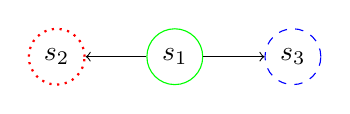
\begin{tikzpicture}

\node[circle, draw=green] at (0,0) (a) {$s_1$};
\node[circle, draw=red, dotted, thick] at (-1.5,0) (b)  {$s_2$};
\node[circle, draw=blue, dashed] at (1.5,0) (c)  {$s_3$};

\draw[->] (a)->(b);
\draw[->] (a)->(c);
\end{tikzpicture}
}
\qquad\qquad
\begin{minipage}{1.2in}%

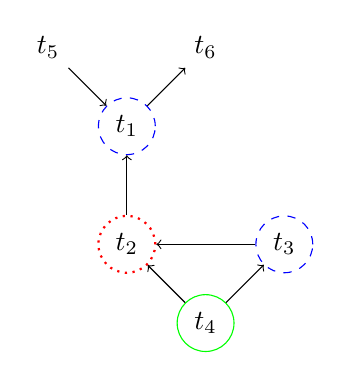
\begin{tikzpicture}
\node[circle, draw=green] at (0,0) (blue) {$t_4$};
\node[circle, draw=red, dotted, thick] at (-1,1) (green) {$t_2$};
\node[circle, draw=blue, dashed] at (1,1) (yellowone) {$t_3$};
\node[circle, draw=blue, dashed] at (-1,2.5) (yellowtwo) {$t_1$};
\node at (-2,3.5) (redone) {$t_5$};
\node at (-0,3.5) (redtwo) {$t_6$};

\draw[->] (blue) -> (green);
\draw[->] (blue) -> (yellowone);
\draw[->] (yellowone) -> (green);
\draw[->] (green) -> (yellowtwo);
\draw[->] (redone) -> (yellowtwo);
\draw[->] (yellowtwo) -> (redtwo);


\end{tikzpicture}
\end{minipage}
\caption{After vertex placements $s_1 \to t_4$ and $s_2 \to t_2$, the domain for vertex $s_3$ would normally be $\{t_1, t_3\}$. However, by checking for reachability from $t_4$ we can reduce this to $\{t_3\}$. The numbers represent the matching order and the circle styles represent labels.}
\label{fig:reachability-filtered}
\end{figure}
\subsection{Reachability of neighbourhood \hspace{12pt}(N-filtering)}
In addition to filtering domains based on the current partial matching and the source- and target graph, we can perform domain filtering based on domains that are already computed by other methods. If some source graph vertex $s_1$ with domain $D_1$ has an edge to some vertex $s_2$ with domain $D_2$, then for each target graph vertex $t_1 \in D_1$ there must exist a path to some vertex $t_2 \in D_2$. If not, then $t_1$ may be removed from $D_1$. This process yields new (smaller) domains and is therefore repeated until a fixed point is reached.

\begin{minipage}{\textwidth}
\begin{defn}[compatibility under neighbourhood reachability constraint]

If $M$ is the current partial mapping and $P$ is the set of paths in the target graph, then neighbourhood reachability compatibility is defined as $$\mathit{compatible}_{\mathit{N-REACH}}(s,t):= \lim_{i\to\infty} \mathit{nreach}_i(s, t) $$

$$\text{where:}$$

$$\mathit{nreach}_i(s, t) = \begin{cases}
                \mathit{compatible}_{\mathit{M-REACH}}(s,t)   & i = 0\\
               \mathit{ncomp}_i^{\mathit{pred}}(s, t) \land \mathit{ncomp}_i^{\mathit{succ}}(s, t) & \text{otherwise}
           \end{cases}$$

\vspace{10pt}

\begin{tabular}{lll}
\centering
$\mathit{ncomp}_i^{\mathit{pred}}(s, t) := $&\multicolumn{2}{l}{$\forall s' \in \mathit{pred}(s) . \exists t' \in V_T . \mathit{nreach}_{i-1}(s',t') \land $}\\
&$\exists p \in P .$  & $\mathit{first}(p)=t' \land$ \\
&&$\mathit{last}(p)=t \land$ \\
&&$\mathit{intermediate}(p) \cap M = \emptyset$
\end{tabular}

\begin{tabular}{lll}

$\mathit{ncomp}_i^{\mathit{succ}}(s, t) := $&\multicolumn{2}{l}{$\forall s' \in \mathit{succ}(s) . \exists t' \in V_T . \mathit{nreach}_{i-1}(s',t') \land $}\\
&$\exists p \in P .$  & $\mathit{first}(p)=t \land$ \\
&&$\mathit{last}(p)=t' \land$ \\
&&$\mathit{intermediate}(p) \cap M = \emptyset$
\end{tabular}

\end{defn}
\end{minipage}

\section{Pruning methods}
\label{sec:pruningmethods}
\subsection{ZeroDomain pruning}
%applicable to both isomorphism and homeomorphism
The ZeroDomain pruning method decides to backtrack if and only if one of the domains is empty, i.e. there exists some source graph vertex that cannot be matched with any target graph vertex. A homeomorphism cannot be found in the current search branch as no potential match exists for this source graph vertex. An example of a domain assignment where ZeroDomain prunes the search space is shown in Table \ref{tab:zerodomain}.

\label{sec:emptyDomain}
\begin{table}
\centering
\begin{tabular}{|l|l|}
\hline
\textbf{Source graph vertex} & \textbf{Target graph candidates} \\ \hline
$s_1$                          & $\{t_1, t_3, t_5\}$         \\ \hline
$s_2$                          & $\{t_1, t_2, t_3, t_4\}$       \\ \hline
$s_3$                          & $\{t_2, t_3, t_6\}$      \\ \hline
$s_4$                          & $\emptyset$                      \\ \hline
\end{tabular}
\caption{If the empty domain pruning method detects an empty target graph domain for some source graph vertex, backtracking is initiated. This is the case if the possible target graph candidates are as shown as in this table.}
\label{tab:zerodomain}
\end{table}

\subsection{AllDifferent pruning}
\label{sec:alldifferent}
The AllDifferent constraint specifies that every variable should be able to have a different value. This is the case with some variable having an empty domain, but also in other cases (i.e. AllDifferent is stronger than ZeroDomain). Since a homeomorphism requires such an assignment, the AllDifferent pruning algorithm backtracks in this case. Alldifferent uses quadratic space since each domain needs to be known at the same time (in contrast with zero-domain, in which the knowledge of each domain separately is sufficient). An example of a domain assignment where AllDifferent prunes the search space but ZeroDomain does not is shown in Table \ref{tab:alldifferent}. 

\begin{table}
\centering
\begin{tabular}{|l|l|}
\hline
\textbf{Source graph vertex} & \textbf{Target graph candidates} \\ \hline
$s_1$                          & $\{t_1, t_2, t_3\}$      \\ \hline
$s_2$                          & $\{t_1, t_2\}$              \\ \hline
$s_3$                          & $\{t_2, t_3\}$              \\ \hline
$s_4$                          & $\{t_1, t_3\}$             \\ \hline
\end{tabular}
\caption{In this example, four source graph vertices have a total domain of only three target graph candidates. By the pigeonhole principle, no injective assignment is possible. AllDifferent recognises this and initiates backtracking.}
\label{tab:alldifferent}
\end{table}




\section{When to apply}
When a pruning method has been selected and a strategy to obtain the domains, one must lastly decide when to apply the pruning method.
\subsection{Runtime calculation}
The simplest option is to calculate the domains and run the pruning strategy each time a vertex is selected for usage in a matching. This could be a target graph vertex that is selected as for vertex-on-vertex matching or a target graph vertex that is part of a path in edge-on-path matching. This changes the partial matching and thus the domains. The pruning method then decides to allow it or to disallow it.
\subsection{Caching domains - incremental domain calculation}
Another option is to cache the domain of each variable and update it based on the current partial matching. This saves valuable time but requires quadratic space\footnote{i.e. some constant $c$ exists such that the space required has an upper bound of $c * |V_{target}|^2$} (for each source graph vertex $\in |V_{source}|$ it needs to store a domain of average size $O(|V_{target}|)$). If M-reachability filtering or N-reachability filtering is used, paths need to be cached as well. That is, for each edge $\in E_{source}$ we need to store a path of $O(|V_{target}|)$ vertices.
\subsection{Parallel calculation}
Finally, we can perform the domain filtering and procedure in a seperate CPU thread while the algorithm continues without backtracking. The pruning thread queries the current matching and calculates whether pruning is appropriate for that matching. If it decides that it is not, it requeries the current matching. Otherwise, it will interrupt the main thread and signal it to backtrack until the pruning method does not detect a dead branch anymore. This method cannot perform caching, since that requires updating the cache \textit{every} time the partial matching is extended - and performance benefits are only gained when the partial matching is only occasionally queried.

\chapter{Business case: Lattic ECP5}
We will apply our algorithm to map virtual FPGAs to the concrete Lattice ECP5 FPGA. An image of this FPGA on an evaluation board is shown in Figure \ref{fig:evaluationboard}. This FPGA's architecture consists of `tiles' of different types in a grid pattern. Each of these tiles has an associated x- and y-coordinate in the grid system and is (generally) topologically the same as tiles of the type elsewhere in the grid. There exists I/O tiles which' function is to retrieve and send data from outside the FPGA, DSP tiles that perform signal processing calculations, tiles that only provide routing structure, RAM tiles and tiles that are internally used for clock management and configuration.

\begin{figure}
\centering
\includegraphics[width=0.5\textwidth]{images/ECP5.png}
\caption[Evaluation board of the LFE5UM5G-85F FPGA: a variant of the ECP5.]{Evaluation board of the LFE5UM5G-85F FPGA: a variant of the ECP5.\footnotemark}
\label{fig:evaluationboard}
\end{figure}
\footnotetext{\texttt{http://www.latticesemi.com/products/developmentboardsandkits/ecp5evaluationboard}, accessed July 10th 2020}	

The structure of an ECP5 FPGA is shown in Figure \ref{fig:ecp5architecture}. This figure shows the grid/tile structure of the ECP5 along with specific components from the electrical engineering domain. The largest portion of the grid structure are logic tiles that contain 8 LUTs and 8 registers (or flip-flops (FF)), bundled in 4 modules. We will focus on this type of tile to find homeomorphisms. We used Project Trellis \cite{trellis} to obtain graphs of both an individual tile (shown in Figure \ref{fig:ECPTGephi}) and of collections of adjacent tiles.

\begin{figure}
\centering
\includegraphics[width=0.8\textwidth]{images/ECP5Architecture.png}
\caption[Architecture of the ECP5 FPGA. Note that it is tile-based in a square grid structure]{Architecture of the ECP5 FPGA. Note that it is tile-based in a square grid structure.\footnotemark}
\label{fig:ecp5architecture}
\end{figure}
\footnotetext{ECP5\texttrademark and ECP5-5G\texttrademark Family Data Sheet (FPGA-DS-02012 Version 1.9), accessed October 1st 2020}	

The virtual FPGA we aim to emulate on this board (which we will call \textit{VirBoard}) is one that, like the ECP5 consists of a tile-like structure with no wires spanning no more than a single tile. Because of this limitation, a student may freely drag-and-drop functionality in the virtual environment without worrying about implicitly overlapping connections. Each tile in this virtual FPGA has significantly less functionality than one of the ECP5. It has a single in- and output at each compass direction, a 2-bit LUT and an 1-bit register. It can be configured in several ways:

\begin{enumerate}
\item As a single wire from one compass direction to the opposite
\item As a cross-section of two orthogonal wires
\item A wire from direction A making a 90 degree turn to direction B, and a wire from direction B to the opposite direction of A.
\item As a configurable 2-input-2-output LUT with any two compass directions as inputs and the other two as outputs
\item As an 1-bit register with any compass direction as data input, any other compass direction as clock-enable (allowing the register value to be set) and any single remaining compass direction as register output. The final compass direction outputs the input of the register.
\end{enumerate}

These different configurations are visualised in Figure \ref{fig:virboardconfigs}.

\begin{figure}
\centering
\includegraphics[width=0.8\textwidth]{images/virboard.png}
\caption{All five possible configurations of VirBoard.}
\label{fig:virboardconfigs}
\end{figure}	

There are countless ways to model this functionality using wires, transistors and logic cells, each of which would yield working emulations if a subgraph homeomorphism of the model is found in the graph model of the concrete FPGA. In principle, one could enumerate all such models and attempt to find subgraph homeomorphisms with each of them, maximizing the expected result. For the scope of our research, however, we limit ourselves to a single graph model that performs well for subgraph homeomorphism search. For this purpose, we design the model of the virtual FPGA with two goals in mind:

\begin{enumerate}
\item It contains as few vertices and edges as possible, so that the search space is as small as possible.
\item It contains as few rare resources as possible, so that more subgraph homeomorphisms are present.
\end{enumerate}

We designed a graph model of VirBoard that encompasses all listed functionality and contains a total of 30 vertices and 32 edges. We were not able to produce a smaller model or one that uses fewer resources. This graph model of VirBoard is shown in Figure \ref{fig:virboard}.



\begin{figure}
\centering
\includegraphics[width=\textwidth]{images/virtualFPGA2.png}
\caption{A graph model of a single cell of the virtual FPGA aimed to emulate on the Lattice ECP5}
\label{fig:virboard}
\end{figure}	

\begin{figure}
\centering
\includegraphics[width=1\textwidth]{images/gephiScreenshot.png}
\caption{Graph model of a single ECP5 logic tile (out of $\pm$42000 logic tiles). Transistors are purple, logical units are red, ports are blue, wires are orange (except those that are neighbouring an adjacent cell, which are brown).}
\label{fig:ECPTGephi}
\end{figure}





\chapter{Performance experiments}
Using a machine with an AMD Ryzen 5 3600 CPU @ 3.7GHz and 32GB 3200MHz memory\footnote{Comparitive experiments were sometimes run on a machine with different specifications} we conduct several experiments with different inputs and settings. For this purpose, we generate random pairs of source graph- and target graph that have subgraph homeomorphisms in them and random pairs that do not.

Firstly, we pose a method for generating random graphs representing virtual FPGAs that adhere to our FPGA modeling methodology:

\begin{enumerate}
\item From $|V|$ we establish how many wires, transistors, logic cells and ports it needs to have the same distribution as the virtual FPGA.
\item We apply the appropriate labels to the vertex set as specified in Chapter \ref{chapter:models}.
\item We connect each port to a random logic cell in a random direction (except the \texttt{CE} port which has to be an input). If the graph is so small there is no logic cell, we add a single one.
\item We connect each port to a random wire in the appropriate direction.
\item We connect each transistor vertex to two different random wire vertices (one with an incoming edge and the other with an outgoing edge).
\end{enumerate}

Since vertex disjoint subgraph homeomorphisms are rare in random graph pairs, we artificially construct source graph-target graph pairs such that it is guaranteed a subgraph homeomorphism exists:

\begin{enumerate}
\item First, we generate a random source graph with $V_S$ vertices using the 5-step method described above.
\item Then, we establish a distribution of $|V_T|$ wires, transistors, logic cells and ports we need to add to resemble the FPGA use case target graph distribution as closely as possible, and add missing vertices to the source graph such that the total vertex set encompasses the established distribution.
\item We apply the appropriate labels to these extra vertices as specified in Chapter \ref{chapter:models}.
\item We connect each new port vertex to a random logic cell vertex, prioritizing new logic cell vertices over existing ones while the new logic cell vertices have a lower average degree. Furthermore, we connect each new port vertex to a random wire in the appriopriate direction.
\item We use half of the extra wires to intersect existing connections. With each intersection equally likely, we intersect a $(\mathtt{WIRE} \to \mathtt{ARC} \to \mathtt{WIRE})$-connection into a $(\mathtt{WIRE} \to \mathtt{ARC} \to \mathtt{WIRE} \to \mathtt{ARC} \to \mathtt{WIRE})$-connection, intersect a $(\mathtt{PORT} \to \mathtt{WIRE})$-connection into a $(\mathtt{PORT} \to \mathtt{WIRE} \to \mathtt{ARC} \to \mathtt{WIRE})$-connection or intersect a  $(\mathtt{WIRE} \to \mathtt{PORT})$-connection into a $(\mathtt{WIRE} \to \mathtt{ARC} \to \mathtt{WIRE} \to \mathtt{PORT})$-connection.
\item We connect each remaining transistor vertex to two different random wire vertices (one with an incoming edge and the other with an outgoing edge), connecting with at least one new wire vertex while the new wire vertices have a lower average degree.
\end{enumerate}

Using this method we obtain random test cases that resemble the graphs of the FPGA use case as closely as possible while still introducing some randomness that allow us to benchmark our algorithm's performance under a variety of optimisations.

Firstly, we compare the different methods of path iteration. The time taken to find a homeomorphism gives an indication of the overhead introduced by a path iterator and also taking the heuristic value of that path iterator into account. This comparison is shown in Figure \ref{fig:pathiterator-performance}. We compare the K-path, control point (CP), DFS, Greedy cached DFS (GDFS C), greedy in-place DFS using a distance metric (GDFS O IP) and greedy in-place DFS using a partial-mapping-aware distance metric (GDFS A IP) path iteration methods. We used target graphs that were respectively 50\%, 200\% and 400\% larger than the souce graph\footnote{In the FPGA use case the target graph is $\pm$ 97 times larger than the souce graph. This, however, is too computationally expensive for our testing methodology.}. We also add the performance of a portfolio method: running the algorithm in parallel with each path iteration method and choosing the fastest outcome for each individual test case. We measure the space usage of each path iterator, the results of which are shown in Figure \ref{fig:spaceusage-pathiterators}.

Without optimisations, we observe exponential behaviour with approximate complexity$O(e^{0.7*|V_S|})$ for $|V_T|=1\frac{1}{2}|V_S|$, $O(e^{1.0482*|V_S|})$ for $|V_T|=3|V_S|$ and $O(e^{1.133*|V_S|})$ for $|V_T|=5|V_S|$. Extrapolating this to the FPGA use case where $|V_T|=97|V_S|$ assuming a logarithmic trend, we get a scalability of $\pm O(e^{2.57442*|V_S|})$ for our FPGA use case without pruning or contraction.

We measure the performance difference between using GreatestConstrainedFirst as the source graph vertex ordering compared to a random ordering in Figure \ref{fig:greatestConstrainedfirstVersusRandom}. Similarly, we compare the distance-based target graph vertex ordering with a degree-based ordering in Figure \ref{fig:DistanceVersusDegree} and compare the degree-based ordering with a random ordering in Figure \ref{fig:greatestDegreeVersusRandom}.

Next, we measure the performance gain from contraction by plotting the mean time increase or decrease in cases where subgraph homeomorphisms are present in Figure \ref{fig:contraction-performance}. Similarly, we measure the performance gain from each method of pruning (pruning technique, filtering and application) compared to applying no pruning at all in Figures \ref{fig:zerodomainlabelsneighbours} through \ref{fig:alldifferentNfiltering} and measure its impact on space usage in Figures {\color{red} TODO: make figure}

Lastly, we take the optimal set of settings and measure for each path iteration method how long the algorithm on average takes to find a subgraph homeomorphism where one exists.



\begin{figure}
\begin{subfigure}{.5\linewidth}
\centering

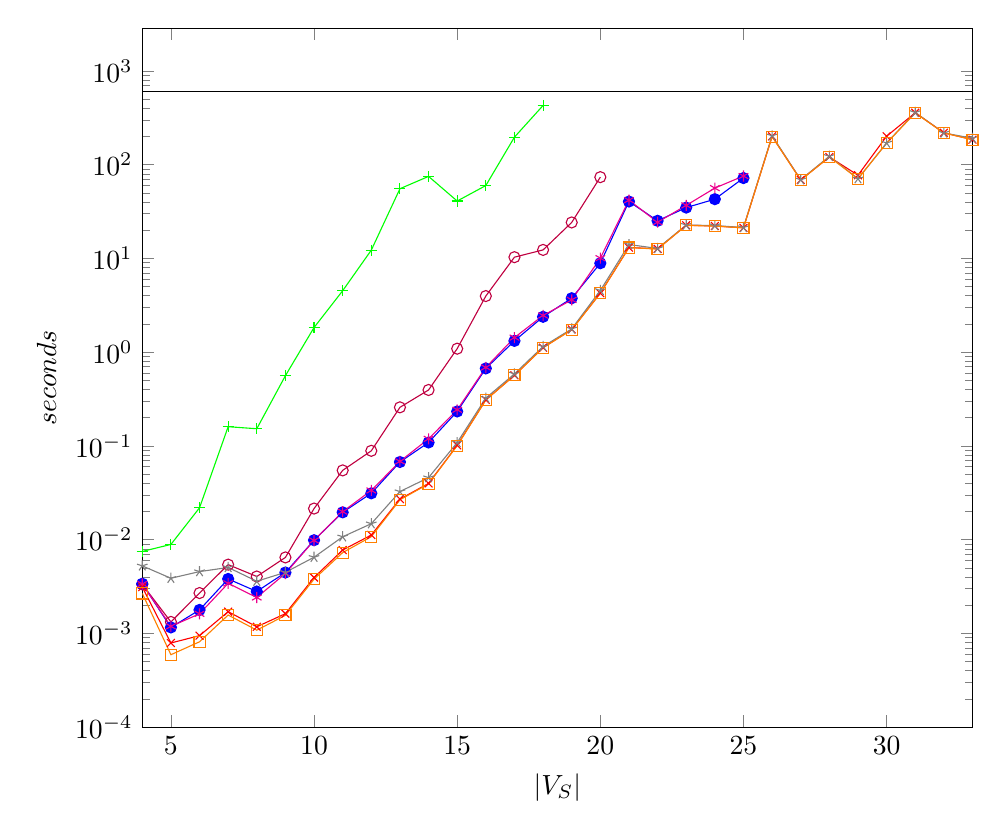
\begin{tikzpicture}
    \begin{axis}[
        xlabel=$|V_S|$,
        ylabel=$seconds$,
        ymin=0.0001,
        ymode=log,
        xmin=4,
        xmax=33,
        legend style={at={(0.9,0.1)},anchor=south east},
        width=\textwidth,
    ]
    
\addplot[
        mark=none,
        black,
    ] plot coordinates {
        (4,600)
        (33,600)
};
 %   \addlegendentry{Timeout 10m} 
    

    
   \addplot[
        mark=o,
        purple,
    ] plot coordinates {
        (4,0.0033354099999999996)
        (5,0.001327198)
        (6,0.0026972415)
        (7,0.005420836)
        (8,0.004050544)
        (9,0.006470579)
        (10,0.021485644)
        (11,0.0548721365)
        (12,0.0887547805)
        (13,0.258150266)
        (14,0.39556562399999995)
        (15,1.0907645185)
        (16,3.971699851282051)
        (17,10.321538780851064)
        (18,12.337433302040818)
        (19,24.217103684000005)
        (20,73.71199097)
};
%    \addlegendentry{GDFS O IP}
    
    
    
    \addplot[
        mark=+,
        green,
    ] plot coordinates {
        (4,0.0074964425000000005)
        (5,0.008899364)
        (6,0.021902257999999997)
        (7,0.160471234)
        (8,0.15263485899999998)
        (9,0.561916418)
        (10,1.833818564)
        (11,4.52718843880597)
        (12,12.26901466122449)
        (13,55.44448909999999)
        (14,75.0789921)
        (15,40.98504065555555)
        (16,59.94558265)
        (17,196.817508975)
        (18,428.4561328)
};
 %   \addlegendentry{CP}
    
    
    \addplot[
        mark=*,
        blue,
    ] plot coordinates {
        (4,0.0033891155)
        (5,0.0011595824999999999)
        (6,0.0017819205)
        (7,0.0038146409999999997)
        (8,0.0028014885)
        (9,0.004467115)
        (10,0.0098760425)
        (11,0.019585361000000003)
        (12,0.031251991)
        (13,0.067427614)
        (14,0.108922384)
        (15,0.233365984)
        (16,0.6713743385)
        (17,1.3210855519999998)
        (18,2.386009026)
        (19,3.765988756140351)
        (20,8.89447237352941)
        (21,40.502501818750005)
        (22,25.221025914285715)
        (23,34.883353815384616)
        (24,42.90160877142857)
        (25,72.07346983333335)
};
%    \addlegendentry{K-Path}
    
    \addplot[
        mark=asterisk,
        magenta,
    ] plot coordinates {
        (4,0.0033671915)
        (5,0.001190538)
        (6,0.0016191069999999998)
        (7,0.0034239325)
        (8,0.0024179585)
        (9,0.0043627885)
        (10,0.009817592)
        (11,0.019897870499999998)
        (12,0.0335268765)
        (13,0.068505526)
        (14,0.1189895675)
        (15,0.2430346145)
        (16,0.6879985279999999)
        (17,1.4320328555000001)
        (18,2.4644637565)
        (19,3.615006598192771)
        (20,10.072892529508197)
        (21,41.85573263125)
        (22,24.362516080952382)
        (23,36.84446636538462)
        (24,56.330943354545454)
        (25,75.77811247500001)
};
%    \addlegendentry{GDFS A IP}
    
    \addplot[
        mark=x,
        red,
    ] plot coordinates {
        (4,0.003124064)
        (5,7.913285000000001E-4)
        (6,9.468475E-4)
        (7,0.0017073364999999998)
        (8,0.0011771495)
        (9,0.0016255140000000002)
        (10,0.0039480825)
        (11,0.0077563585)
        (12,0.0112181135)
        (13,0.027106744)
        (14,0.039854954500000005)
        (15,0.1016730035)
        (16,0.3102863915)
        (17,0.567070922)
        (18,1.1181295875)
        (19,1.7503998269999999)
        (20,4.263310112765957)
        (21,13.087688980434784)
        (22,12.664759238095238)
        (23,22.604950978378376)
        (24,22.215862426666664)
        (25,21.221224975862068)
        (26,200.80231476666665)
        (27,69.01728853)
        (28,120.91195150000003)
        (29,77.2825083)
        (30,201.28251479999994)
        (31,358.3321691)
        (32,219.1503222)
        (33,184.9894481)
};
 %   \addlegendentry{DFS}
    
    \addplot[
        mark=star,
        gray,
    ] plot coordinates {
        (4,0.0052584419999999995)
        (5,0.0038800225)
        (6,0.0045671005)
        (7,0.005054851500000001)
        (8,0.0036043110000000002)
        (9,0.0044851380000000005)
        (10,0.006500158000000001)
        (11,0.010743765999999998)
        (12,0.014813136499999999)
        (13,0.032617665)
        (14,0.045932047000000004)
        (15,0.10862769200000001)
        (16,0.32415647649999996)
        (17,0.586893169)
        (18,1.1500186795)
        (19,1.772846179)
        (20,4.554298787121212)
        (21,14.077475467441861)
        (22,12.78838592857143)
        (23,22.725297256756754)
        (24,22.44824257)
        (25,21.37612426551724)
        (26,203.35969063333334)
        (27,69.08358688)
        (28,123.07605716000003)
        (29,70.88854776666666)
        (30,170.599628675)
        (31,361.26002704999996)
        (32,217.99103095)
        (33,191.6499955)
};
%    \addlegendentry{GDFS C}
    
    \addplot[
        mark=square,
        orange,
    ] plot coordinates {
        (4,0.0026720765000000004)
        (5,5.931255E-4)
        (6,8.145884999999999E-4)
        (7,0.0015716150000000002)
        (8,0.001083881)
        (9,0.0015602699999999999)
        (10,0.0037946819999999997)
        (11,0.0072780025)
        (12,0.010769405999999999)
        (13,0.026622686)
        (14,0.039441741499999995)
        (15,0.1005090725)
        (16,0.3088769205)
        (17,0.5658370635)
        (18,1.114951387)
        (19,1.7321635599999998)
        (20,4.2505378978723405)
        (21,13.068786297826087)
        (22,12.589129547619047)
        (23,22.530537545945947)
        (24,22.130406946666668)
        (25,21.19573636896552)
        (26,199.31648383333334)
        (27,68.44248519)
        (28,120.89257580000003)
        (29,70.80782896666666)
        (30,169.777134475)
        (31,356.8092052)
        (32,217.99103095)
        (33,184.9894481)
};
 %   \addlegendentry{portfolio}

    \end{axis}
    \end{tikzpicture}

\caption{$|V_T|=1\frac{1}{2}|V_S|$}
\label{fig:sub1}
\end{subfigure}%
\begin{subfigure}{.5\linewidth}
\centering

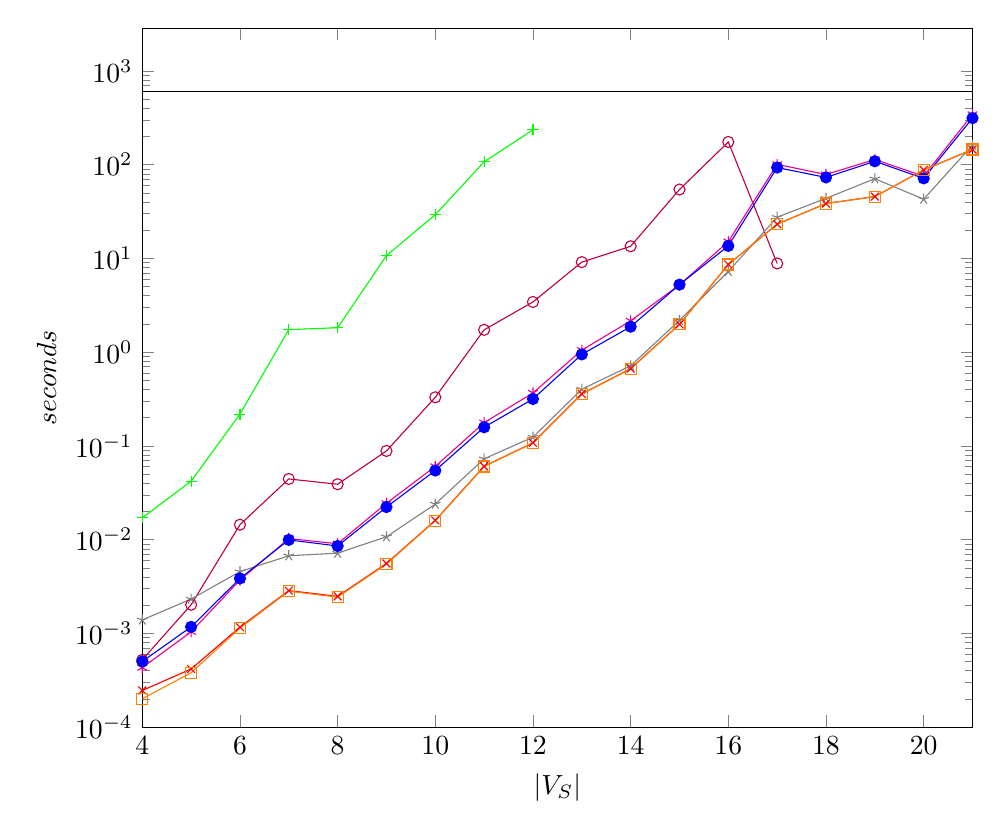
\begin{tikzpicture}
    \begin{axis}[
        xlabel=$|V_S|$,
        ylabel=$seconds$,
        ymin=0.0001,
        ymode=log,
        xmin=4,
        xmax=21,
        legend style={at={(0.9,0.1)},anchor=south east},
        width=\textwidth,
    ]
    
\addplot[
        mark=none,
        black,
    ] plot coordinates {
        (4,600)
        (21,600)
};
 %   \addlegendentry{Timeout 10m} 
    

\addplot[
        mark=+,
        green,
    ] plot coordinates {
        (4,0.017118874)
        (5,0.042044554000000005)
        (6,0.21861366149999997)
        (7,1.7413124975)
        (8,1.824231057)
        (9,10.718911422807018)
        (10,29.285856038095236)
        (11,107.36171433333334)
        (12,235.52224905)
};
%    \addlegendentry{CP}
    
    
    \addplot[
        mark=o,
        purple,
    ] plot coordinates {
        (4,5.229545E-4)
        (5,0.0020221634999999997)
        (6,0.014452913000000001)
        (7,0.044465508)
        (8,0.039038954)
        (9,0.088448429)
        (10,0.33017173499999997)
        (11,1.7330093685)
        (12,3.436815223163842)
        (13,9.139001624999999)
        (14,13.487728657446809)
        (15,54.37308013571429)
        (16,174.90209208000002)
        (17,8.8468752)
};
%    \addlegendentry{GDFS O IP}
    
    \addplot[
        mark=star,
        gray,
    ] plot coordinates {
        (4,0.00139258)
        (5,0.002327794)
        (6,0.004565538)
        (7,0.0067396635000000005)
        (8,0.0071890365)
        (9,0.010737805)
        (10,0.02400474)
        (11,0.07292148550000001)
        (12,0.12421214450000001)
        (13,0.403000701)
        (14,0.7163419985)
        (15,2.1890222930000003)
        (16,7.270705493975904)
        (17,27.538684308695654)
        (18,43.79655899583333)
        (19,70.8624523888889)
        (20,42.929491375)
        (21,161.7936666)
};
 %   \addlegendentry{GDFS C}
    
    \addplot[
        mark=x,
        red,
    ] plot coordinates {
        (4,2.463635E-4)
        (5,4.17268E-4)
        (6,0.001167168)
        (7,0.002865959)
        (8,0.0024855845)
        (9,0.0055816305)
        (10,0.016075872499999998)
        (11,0.060558201)
        (12,0.1081205275)
        (13,0.358527165)
        (14,0.6678748950000001)
        (15,1.9833789535)
        (16,8.623507047058824)
        (17,23.20956361923077)
        (18,38.53969741666666)
        (19,45.70503912307693)
        (20,88.00206148888888)
        (21,145.2799635)
};
%    \addlegendentry{DFS}
    
    
    \addplot[
        mark=asterisk,
        magenta,
    ] plot coordinates {
        (4,4.3166750000000006E-4)
        (5,0.0010404115)
        (6,0.003709151)
        (7,0.010290998499999999)
        (8,0.009050423)
        (9,0.0244776325)
        (10,0.060524060500000004)
        (11,0.177295532)
        (12,0.36728383800000003)
        (13,1.0505953314999998)
        (14,2.158745016)
        (15,5.232621873043478)
        (16,15.130776390697672)
        (17,100.89787280000002)
        (18,78.64249841111112)
        (19,113.64276582222222)
        (20,75.4335271625)
        (21,343.9340747)
};
%    \addlegendentry{GDFS A IP}
    
    \addplot[
        mark=*,
        blue,
    ] plot coordinates {
        (4,5.025650000000001E-4)
        (5,0.0011748805)
        (6,0.0038617564999999998)
        (7,0.009955469500000001)
        (8,0.008569285)
        (9,0.022299932)
        (10,0.054706759)
        (11,0.158324873)
        (12,0.317071005)
        (13,0.9476776635)
        (14,1.870529588)
        (15,5.256302935245901)
        (16,13.612862210869567)
        (17,93.2565386888889)
        (18,73.17322655555556)
        (19,108.78198909999999)
        (20,71.5219922)
        (21,314.1443365)
};
%    \addlegendentry{K-Path}
    
    \addplot[
        mark=square,
        orange,
    ] plot coordinates {
        (4,2.01024E-4)
        (5,3.8098600000000004E-4)
        (6,0.001139124)
        (7,0.0028233219999999996)
        (8,0.00244008)
        (9,0.0054960905)
        (10,0.015953537)
        (11,0.060388840000000006)
        (12,0.107574184)
        (13,0.358221664)
        (14,0.662612554)
        (15,1.9811704315)
        (16,8.621956076470587)
        (17,23.20956361923077)
        (18,38.53969741666666)
        (19,45.70503912307693)
        (20,88.00206148888888)
        (21,145.2799635)
};
 %   \addlegendentry{portfolio}
    

  
    \end{axis}
    \end{tikzpicture}

\caption{$|V_T|=3|V_S|$}
\label{fig:sub2}
\end{subfigure}\\[1ex]
\begin{subfigure}{0.5\linewidth}
\centering

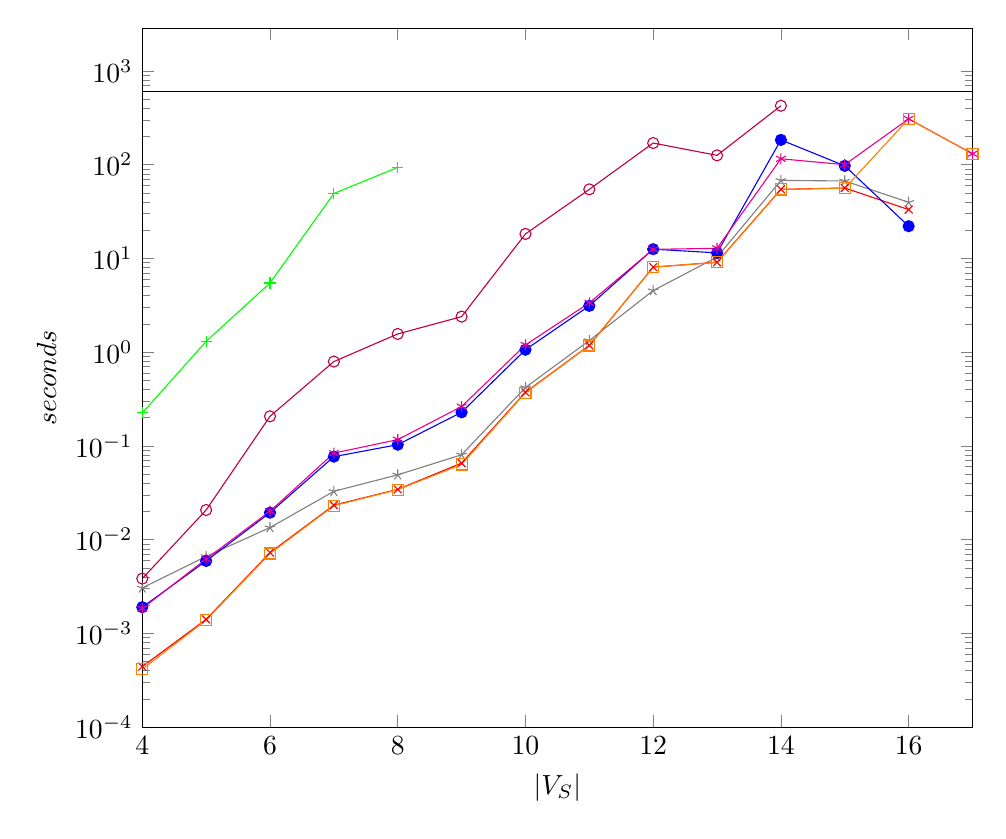
\begin{tikzpicture}
    \begin{axis}[
        xlabel=$|V_S|$,
        ylabel=$seconds$,
        ymin=0.0001,
        ymode=log,
        xmin=4,
        xmax=17,
        legend style={at={(0.9,0.1)},anchor=south east},
        width=\textwidth,
    ]
    
\addplot[
        mark=none,
        black,
    ] plot coordinates {
        (4,600)
        (17,600)
};
 %   \addlegendentry{Timeout 10m} 
    


\addplot[
        mark=+,
        green,
    ] plot coordinates {
        (4,0.22498123849999999)
        (5,1.305544137)
        (6,5.477192146428571)
        (7,49.320910733333335)
        (8,93.62391244)
};
%    \addlegendentry{CP}
    
    
    \addplot[
        mark=star,
        gray,
    ] plot coordinates {
        (4,0.003058187)
        (5,0.0066316019999999995)
        (6,0.013466777000000001)
        (7,0.032822169)
        (8,0.049183345)
        (9,0.080513419)
        (10,0.4200455685)
        (11,1.3332708905000001)
        (12,4.545143440151515)
        (13,10.333796216470589)
        (14,68.03150406)
        (15,67.08428195454545)
        (16,39.747431)
};
%    \addlegendentry{GDFS C}
    
    \addplot[
        mark=x,
        red,
    ] plot coordinates {
        (4,4.4261750000000003E-4)
        (5,0.0014131274999999999)
        (6,0.0072753685000000005)
        (7,0.023372011)
        (8,0.0344219615)
        (9,0.0656533275)
        (10,0.3738274895)
        (11,1.183567724)
        (12,8.084725380597014)
        (13,9.105788104705884)
        (14,54.59190611666667)
        (15,56.45855956363636)
        (16,33.2144619)
};
%    \addlegendentry{DFS}
    
    \addplot[
        mark=*,
        blue,
    ] plot coordinates {
        (4,0.001906137)
        (5,0.005935332)
        (6,0.0194225855)
        (7,0.0768926385)
        (8,0.103136142)
        (9,0.228699563)
        (10,1.062870499)
        (11,3.1228105518134712)
        (12,12.555450586)
        (13,11.474581472222223)
        (14,183.9983442333333)
        (15,97.27099918571427)
        (16,22.0919737)
};
%    \addlegendentry{K-Path}
    
    
    \addplot[
        mark=o,
        purple,
    ] plot coordinates {
        (4,0.0038459365)
        (5,0.020740273)
        (6,0.20711417999999998)
        (7,0.7947821999999999)
        (8,1.565915889)
        (9,2.396293172)
        (10,18.270429463636365)
        (11,54.59309324615385)
        (12,170.3045068)
        (13,125.79853659999999)
        (14,425.516946)
};
%    \addlegendentry{GDFS O IP}
    
    
    \addplot[
        mark=asterisk,
        magenta,
    ] plot coordinates {
        (4,0.0018444635000000001)
        (5,0.006224887500000001)
        (6,0.0201156265)
        (7,0.0838507)
        (8,0.11677660100000001)
        (9,0.2631939955)
        (10,1.195823311)
        (11,3.358671161111111)
        (12,12.508858883333334)
        (13,12.832528379245282)
        (14,115.64856344)
        (15,100.09827916666666)
        (16,308.21460745)
        (17,130.7677965)
};
%    \addlegendentry{GDFS A IP}
    
    
    \addplot[
        mark=square,
        orange,
    ] plot coordinates {
        (4,4.152115E-4)
        (5,0.001389112)
        (6,0.0071271165)
        (7,0.023055476000000002)
        (8,0.034188356)
        (9,0.0634472525)
        (10,0.370240898)
        (11,1.1794381704999999)
        (12,8.077388874626866)
        (13,9.088254795294118)
        (14,54.45241678333334)
        (15,56.29606548181818)
        (16,308.21460745)
        (17,130.7677965)
};
%    \addlegendentry{portfolio}
    
  
    \end{axis}
    \end{tikzpicture}

\caption{$|V_T|=5|V_S|$}
\label{fig:sub3}
\end{subfigure}
\begin{subfigure} {0.5\linewidth}
\centering

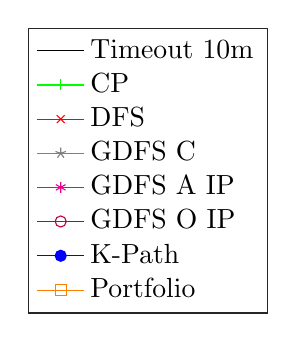
\begin{tikzpicture} 
    \begin{axis}[%
    hide axis,
    xmin=10,
    xmax=50,
    ymin=0,
    ymax=0.4,
    legend style={draw=white!15!black,legend cell align=left}
    ]
	\addlegendimage{black}
    \addlegendentry{Timeout 10m}; 
     
    \addlegendimage{green, mark=+}
    \addlegendentry{CP};
    
    \addlegendimage{red, mark=x}
    \addlegendentry{DFS};
    
    \addlegendimage{gray, mark=star}
    \addlegendentry{GDFS C};
    
    \addlegendimage{magenta, mark=asterisk}
    \addlegendentry{GDFS A IP};
    
    \addlegendimage{purple, mark=o}
    \addlegendentry{GDFS O IP};
    
    \addlegendimage{blue, mark=*}
    \addlegendentry{K-Path};
    
    \addlegendimage{orange, mark=square}
    \addlegendentry{Portfolio};
    \end{axis}
\end{tikzpicture}

\end{subfigure}
\caption{Performance of using different path iterators in test cases with present subgraph homeomorphisms. We avoid unnecessarily long paths, and use no pruning or contraction. We include a portfolio method that takes the best performance rating for each individual test case.}	
\label{fig:pathiterator-performance}
\end{figure}


\begin{figure}
\centering
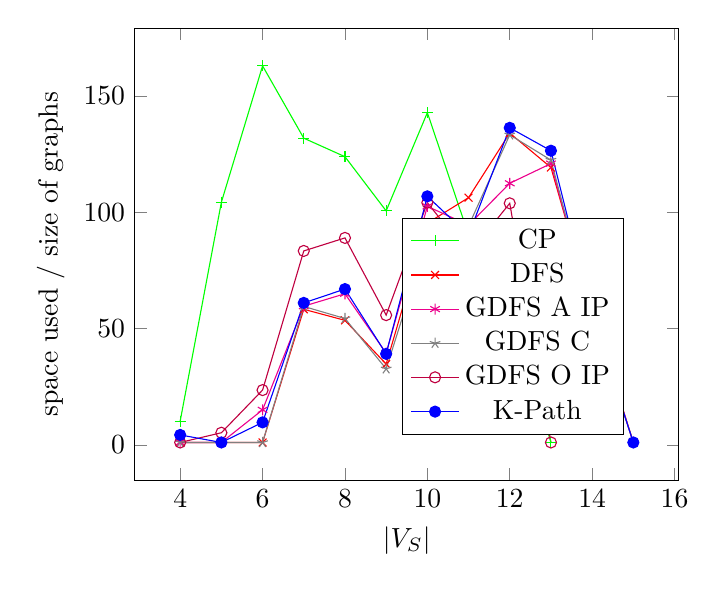
\begin{tikzpicture}
    \begin{axis}[
        xlabel=$|V_S|$,
        ylabel=space used $/$ size of graphs,
        legend style={at={(0.9,0.1)},anchor=south east},
        width=0.7\textwidth,
		%y tick label style={/pgf/number format/sci},
    ]

%    \node[] at (axis cs: 9,1.1) {Awaiting test results (CAES server)};

\addplot[
        mark=+,
        green,
    ] plot coordinates {
        (4,10.174505370550349224253838)
        (5,104.28268407548150313423625)
        (6,162.90001905722773387141976)
        (7,131.82092679714642689897069)
        (8,123.86131153662219616440982)
        (9,100.54876902079979411614113)
        (10,142.8055123071906161809092)
        (11,90.23704183358028315864566)
        (12,60.13828770787494509749228)
        (13,1)
};
    \addlegendentry{CP}
    
    \addplot[
        mark=x,
        red,
    ] plot coordinates {
        (4,1)
        (5,1)
        (6,1)
        (7,58.25769782075416109734502296)
        (8,53.49977853854609387401796491)
        (9,34.69315781105574763597362315)
        (10,95.2821470489074655940527300)
        (11,106.247669775327306151566700)
        (12,134.009989654390014925155652)
        (13,119.208253326512152230628507)
        (14,57.5163619146955535818220329)
        (15,1)
};
    \addlegendentry{DFS}

    \addplot[
        mark=asterisk,
        magenta,
    ] plot coordinates {
        (4,1)
        (5,1)
        (6,15.02985034471161930)
        (7,59.59097376035428638)
        (8,64.93368304714666954)
        (9,39.37678578646825642)
        (10,102.493087611314720)
        (11,94.4701670636009438)
        (12,112.425234638110666)
        (13,120.892092891415954)
        (14,56.0582514421801884)
        (15,1)
};
    \addlegendentry{GDFS A IP}
    
    \addplot[
        mark=star,
        gray,
    ] plot coordinates {
        (4,1)
        (5,1)
        (6,1)
        (7,59.479189954442690)
        (8,54.294753873478837)
        (9,32.656874607567579)
        (10,88.62263521222060)
        (11,94.07313175657136)
        (12,133.2439360650590)
        (13,122.4129802403613)
        (14,55.53333167207465)
        (15,1)
};
    \addlegendentry{GDFS C}
    
    \addplot[
        mark=o,
        purple,
    ] plot coordinates {
        (4,1)
        (5,5.1826054759816817)
        (6,23.512962277899220)
        (7,83.341983867316274)
        (8,88.941938162115534)
        (9,55.750056887542679)
        (10,104.1015790897492)
        (11,81.84559512703726)
        (12,103.8155851653250)
        (13,1)
};
    \addlegendentry{GDFS O IP}
    
    \addplot[
        mark=*,
        blue,
    ] plot coordinates {
        (4,4.240778515784331992)
        (5,1)
        (6,9.641524578218709713)
        (7,61.00961187901417579)
        (8,66.94762056230962072)
        (9,39.09244788901674288)
        (10,106.812982924035309)
        (11,90.1677790988596005)
        (12,136.268506857638343)
        (13,126.432468234002608)
        (14,55.5333316720746569)
        (15,1)
};
    \addlegendentry{K-Path}
	
    \end{axis}
    \end{tikzpicture}
    \caption{Space usage of the algorithm with each path iterator relative to the space usage of the input graphs. Unnecessarily long paths are avoided, target vertices are ordered by degree and contraction is disabled.}
    \label{fig:spaceusage-pathiterators}

\end{figure}



%Mean relative time consumption of contraction-enabled subgraph homeomorphism search compared to contraction-disabled for different path iteration methods. For data points below the reference line contraction saves time while for data points above it contraction costs extra time. We handled a maximum of 1000 test cases or 30 minutes per value of $|V_S|$ for each path iteration method.


\begin{figure}
\begin{subfigure}{.5\linewidth}
\centering

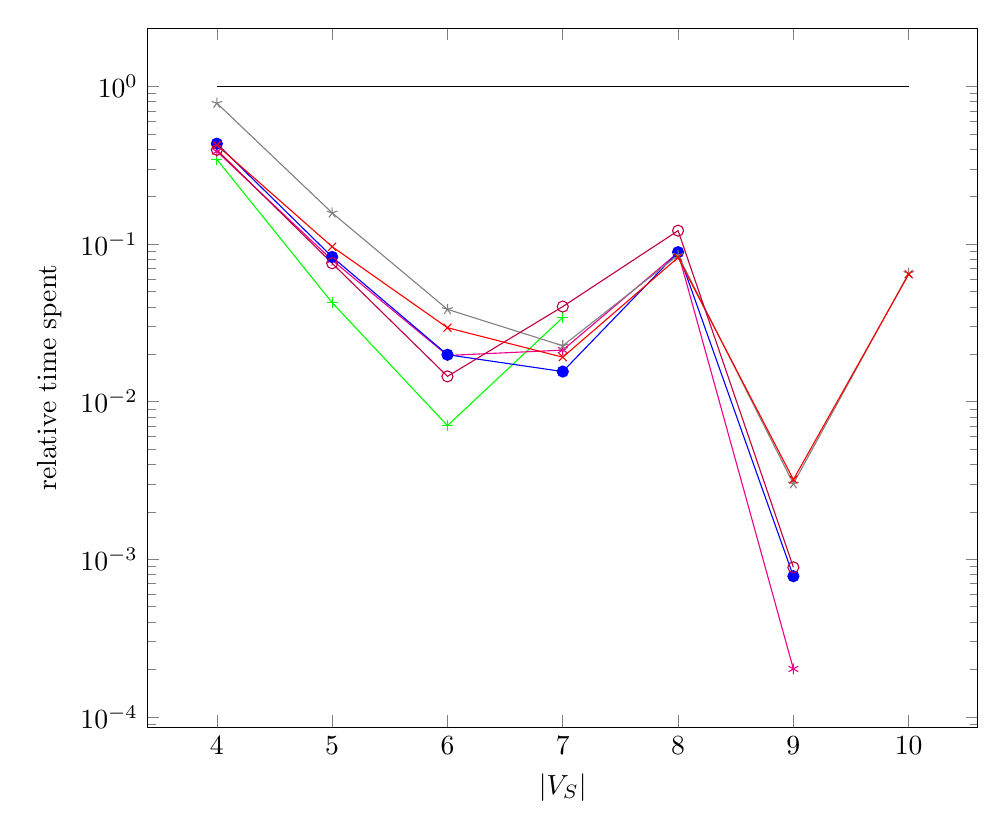
\begin{tikzpicture}
    \begin{axis}[
        xlabel=$|V_S|$,
        ylabel=relative time spent,
        ymode=log,
        legend style={at={(0.9,0.1)},anchor=south east},
        width=\textwidth,
		y tick label style={/pgf/number format/sci},
    ]


\addplot [mark=none, black] plot coordinates {
        (4,1) (10, 1)};
%\addlegendentry{No contraction}
   \addplot[
        mark=+,
        green,
    ] plot coordinates {
        (4,0.34449583915246557)
        (5,0.04250500407360703)
        (6,0.007052140364736389)
        (7,0.034219490143735744)
};
%    \addlegendentry{CP}

\addplot[
        mark=asterisk,
        magenta,
    ] plot coordinates {
        (4,0.38742564587487976)
        (5,0.07909766239343824)
        (6,0.019655091474591525)
        (7,0.021251734957033044)
        (8,0.08842360246711035)
        (9,2.0164236395563237E-4)
};
%    \addlegendentry{GDFS A IP}

\addplot[
        mark=*,
        blue,
    ] plot coordinates {
        (4,0.43377165034858706)
        (5,0.08291766655357158)
        (6,0.019867063872060407)
        (7,0.01553750194233227)
        (8,0.08890227690765527)
        (9,7.816551173891351E-4)
};
%    \addlegendentry{K-Path}

\addplot[
        mark=star,
        gray,
    ] plot coordinates {
        (4,0.7838841422440458)
        (5,0.15772533322419885)
        (6,0.03853822820095056)
        (7,0.02265222193749682)
        (8,0.08504004296545455)
        (9,0.0030177729737449885)
        (10,0.0652985451968477)
};
%    \addlegendentry{GDFS C}

\addplot[
        mark=x,
        red,
    ] plot coordinates {
        (4,0.42425950110101485)
        (5,0.09626130731943527)
        (6,0.029475512058189532)
        (7,0.019168059826692858)
        (8,0.08213870898979722)
        (9,0.00320538172801908)
        (10,0.06429911639723773)
};
%    \addlegendentry{DFS}

\addplot[
        mark=o,
        purple,
    ] plot coordinates {
        (4,0.3963989888723202)
        (5,0.07559274867485685)
        (6,0.014479163749969607)
        (7,0.04015195913379275)
        (8,0.12166475428162647)
        (9,8.901952837352006E-4)
};
%    \addlegendentry{GDFS O IP}


    \end{axis}
    \end{tikzpicture}


\caption{$|V_T|=1\frac{1}{2}|V_S|$}
\label{fig:sub1}
\end{subfigure}%
\begin{subfigure}{.5\linewidth}
\centering

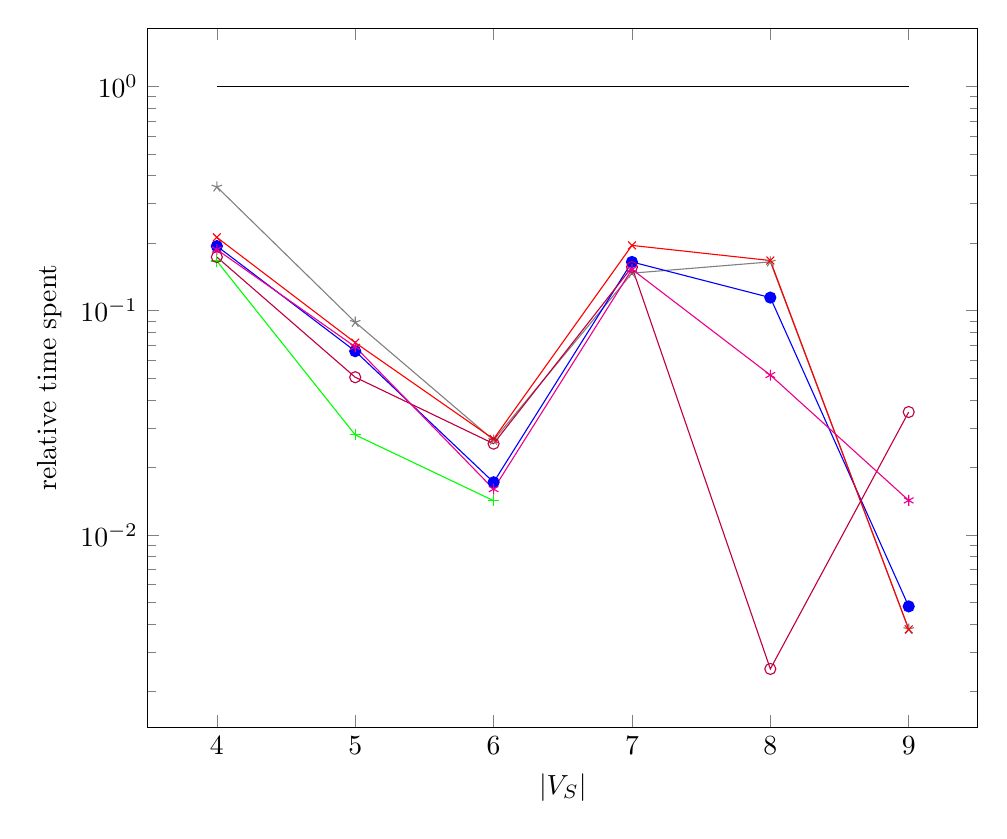
\begin{tikzpicture}
    \begin{axis}[
        xlabel=$|V_S|$,
        ylabel=relative time spent,
        ymode=log,
        legend style={at={(0.9,0.1)},anchor=south east},
        width=\textwidth,
		y tick label style={/pgf/number format/sci},
    ]


\addplot [mark=none, black] plot coordinates {
        (4,1) (9, 1)};
%\addlegendentry{No contraction}

\addplot[
        mark=+,
        green,
    ] plot coordinates {
        (4,0.16656533269519228)
        (5,0.02792481959372131)
        (6,0.014208494420317713)
};
%    \addlegendentry{CP}

\addplot[
        mark=star,
        gray,
    ] plot coordinates {
        (4,0.35670503391181074)
        (5,0.08885285052563148)
        (6,0.02644959281461509)
        (7,0.1469727809071855)
        (8,0.1650715123096471)
        (9,0.003794253797042311)
};
%    \addlegendentry{GDFS C}

\addplot[
        mark=*,
        blue,
    ] plot coordinates {
        (4,0.194158851426724)
        (5,0.06596676865264874)
        (6,0.017166588789163415)
        (7,0.16493104718190343)
        (8,0.11438599305894)
        (9,0.0047972337258095485)
};
%    \addlegendentry{K-Path}

\addplot[
        mark=x,
        red,
    ] plot coordinates {
        (4,0.21233351678836204)
        (5,0.07202295158409817)
        (6,0.026758726043938773)
        (7,0.19551506606564623)
        (8,0.16739005564904727)
        (9,0.003790913734381372)
};
%    \addlegendentry{DFS}

\addplot[
        mark=o,
        purple,
    ] plot coordinates {
        (4,0.17347891126074652)
        (5,0.0504791507537965)
        (6,0.02551664872425517)
        (7,0.15650709939163068)
        (8,0.0025235131787816165)
        (9,0.03532832186507143)
};
%    \addlegendentry{GDFS O IP}

\addplot[
        mark=asterisk,
        magenta,
    ] plot coordinates {
        (4,0.1873514680576187)
        (5,0.06902784077974626)
        (6,0.0160036619729299)
        (7,0.15291763768405797)
        (8,0.0516269965234984)
        (9,0.014247055717867137)
};
%    \addlegendentry{GDFS A IP}
	
	
    \end{axis}
    \end{tikzpicture}

\caption{$|V_T|=3|V_S|$}
\label{fig:sub2}
\end{subfigure}\\[1ex]
\begin{subfigure}{0.5\linewidth}
\centering

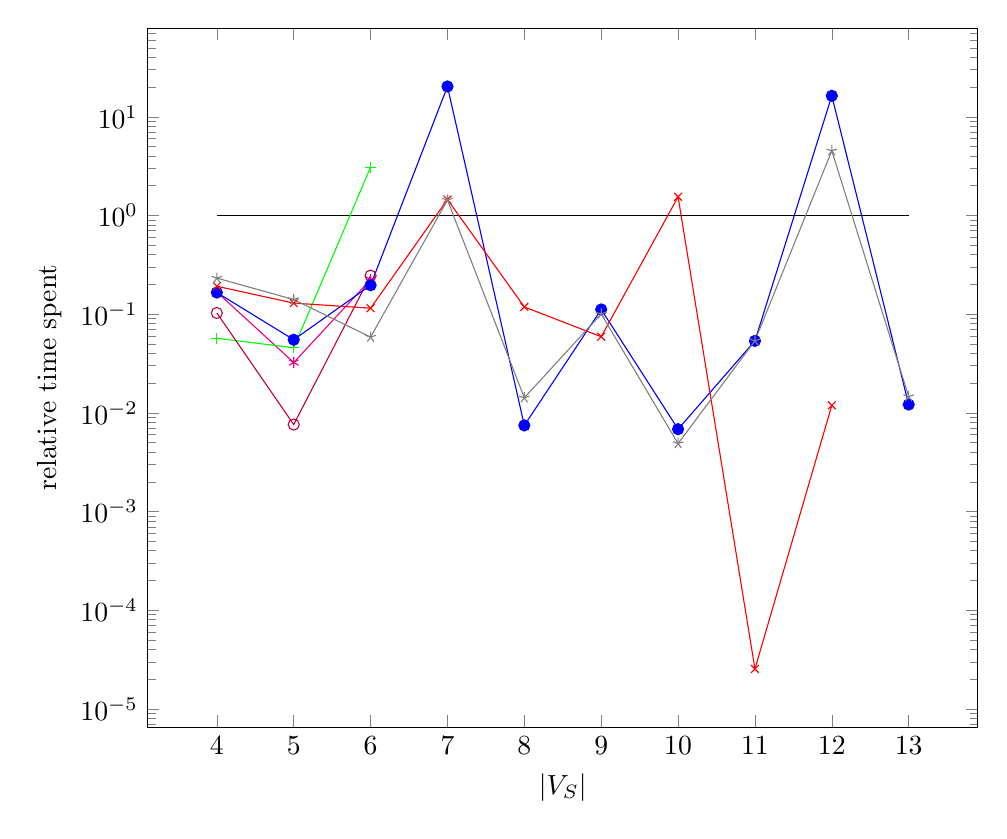
\begin{tikzpicture}
    \begin{axis}[
        xlabel=$|V_S|$,
        ylabel=relative time spent,
        ymode=log,
        legend style={at={(0.9,0.1)},anchor=south east},
        width=\textwidth,
		y tick label style={/pgf/number format/sci},
    ]


\addplot [mark=none, black] plot coordinates {
        (4,1) (13, 1)};
%\addlegendentry{No contraction}

	
\addplot[
        mark=asterisk,
        magenta,
    ] plot coordinates {
        (4,0.1674566113900499)
        (5,0.032349725367020715)
        (6,0.2237865876374895)
};
 %   \addlegendentry{GDFS A IP}
    
    
    \addplot[
        mark=+,
        green,
    ] plot coordinates {
        (4,0.056873208163624955)
        (5,0.04563421043002553)
        (6,3.0895140030860113)
};
 %   \addlegendentry{CP}
    
    \addplot[
        mark=o,
        purple,
    ] plot coordinates {
        (4,0.10276640004366641)
        (5,0.007609829164036706)
        (6,0.24568669245593505)
};
 %   \addlegendentry{GDFS O IP}
    
    \addplot[
        mark=*,
        blue,
    ] plot coordinates {
        (4,0.1655772370426709)
        (5,0.055053818828159615)
        (6,0.19634060714182988)
        (7,20.289869886299307)
        (8,0.007455438509609334)
        (9,0.11168570137538518)
        (10,0.006832180347245251)
        (11,0.053585054708433756)
        (12,16.326793831579934)
        (13,0.01212843469374362)
};
 %   \addlegendentry{K-Path}


\addplot[
        mark=x,
        red,
    ] plot coordinates {
        (4,0.19178983176776473)
        (5,0.1293662743185925)
        (6,0.11496995869605499)
        (7,1.450331503028158)
        (8,0.11835078397595038)
        (9,0.05907513412579321)
        (10,1.545090436667155)
        (11,2.5391954884407796E-5)
        (12,0.011908323973143663)
};
 %   \addlegendentry{DFS}
    
    \addplot[
        mark=star,
        gray,
    ] plot coordinates {
        (4,0.23202692835799185)
        (5,0.14055133962348276)
        (6,0.05857415542176621)
        (7,1.4332274024971468)
        (8,0.014217322662230782)
        (9,0.10041348158626583)
        (10,0.004884744036490124)
        (11,0.053666528274866135)
        (12,4.5260118047084195)
        (13,0.01461043009387195)
};
%    \addlegendentry{GDFS C}
	
	
    \end{axis}
    \end{tikzpicture}

\caption{$|V_T|=5|V_S|$}
\label{fig:sub3}
\end{subfigure}
\begin{subfigure} {0.5\linewidth}
\centering

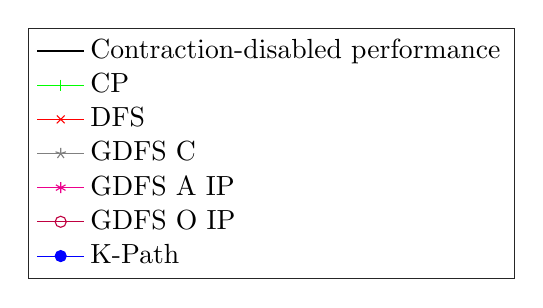
\begin{tikzpicture} 
    \begin{axis}[%
    hide axis,
    xmin=10,
    xmax=50,
    ymin=0,
    ymax=0.4,
    legend style={draw=white!15!black,legend cell align=left}
    ]
	\addlegendimage{black}
    \addlegendentry{Contraction-disabled performance}; 
     
    \addlegendimage{green, mark=+}
    \addlegendentry{CP};
    
    \addlegendimage{red, mark=x}
    \addlegendentry{DFS};
    
    \addlegendimage{gray, mark=star}
    \addlegendentry{GDFS C};
    
    \addlegendimage{magenta, mark=asterisk}
    \addlegendentry{GDFS A IP};
    
    \addlegendimage{purple, mark=o}
    \addlegendentry{GDFS O IP};
    
    \addlegendimage{blue, mark=*}
    \addlegendentry{K-Path};
    
    \end{axis}
\end{tikzpicture}

\end{subfigure}

\caption{Performance of our algorithm with the GreatestConstrainedFirst source graph vertex order relative to the performance of the algorithm with a random source graph vertex order. We avoid unnecessarily long paths, do not perform contraction and use no pruning. Data points above the black reference line denote the GreatestConstrainedFirst ordering introduces more delay, and data points below the reference line denote that it saves time. Note the logarithmic y-axis.}	
\label{fig:greatestConstrainedfirstVersusRandom}
\end{figure}






\begin{figure}
\resizebox{0.28\textheight}{!}{
\begin{subfigure}{.5\linewidth}
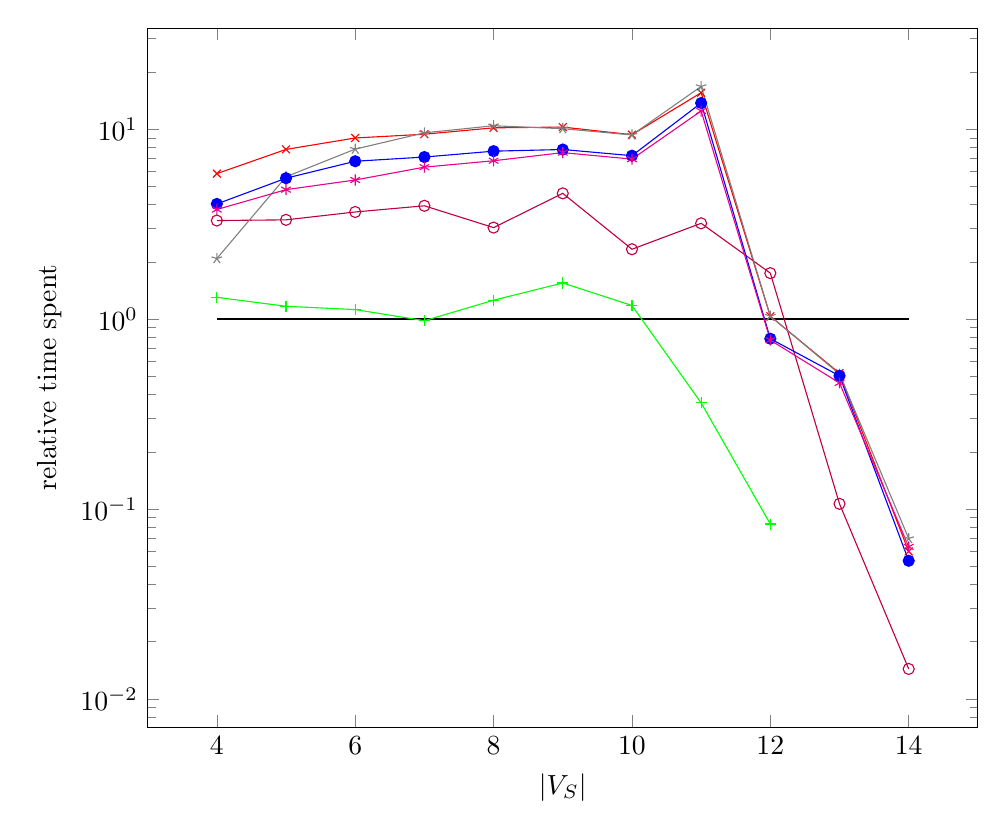
\begin{tikzpicture}
    \begin{axis}[
        xlabel=$|V_S|$,
        ylabel=relative time spent,
        ymode=log,
        legend style={at={(0.9,0.1)},anchor=south east},
        width=\textwidth,
		y tick label style={/pgf/number format/sci},
    ]
\addplot [mark=none, black] plot coordinates {
        (4,1) (14,1)};




\addplot[
        mark=x,
        red,
    ] plot coordinates {
        (4,5.829952304363644)
        (5,7.821514135009583)
        (6,8.982363969917358)
        (7,9.401332680691212)
        (8,10.158832279951605)
        (9,10.252325251025706)
        (10,9.34581888789391)
        (11,15.546748123060839)
        (12,1.0341526662898237)
        (13,0.5183898969146863)
        (14,0.05971709064829511)
};
%    \addlegendentry{DFS}


\addplot[
        mark=o,
        purple,
    ] plot coordinates {
        (4,3.3007473913750918)
        (5,3.3292641262270837)
        (6,3.6622616535723047)
        (7,3.9481137630108396)
        (8,3.030286162147374)
        (9,4.590014716545663)
        (10,2.330905974473567)
        (11,3.192281658331693)
        (12,1.744595348175264)
        (13,0.10640200382876541)
        (14,0.014374937918376296)
};
%    \addlegendentry{GDFS O IP}


\addplot[
        mark=star,
        gray,
    ] plot coordinates {
        (4,2.081240181067252)
        (5,5.613910854682754)
        (6,7.849457219522296)
        (7,9.56049923079753)
        (8,10.416398040783026)
        (9,10.0534722450281)
        (10,9.318833737054117)
        (11,16.77294360448037)
        (12,1.036148432755423)
        (13,0.5131767288245823)
        (14,0.06986347139547233)
};
%    \addlegendentry{GDFS C}


\addplot[
        mark=*,
        blue,
    ] plot coordinates {
        (4,4.036935610516745)
        (5,5.515429351367027)
        (6,6.774063252800069)
        (7,7.129623094348765)
        (8,7.656237850184846)
        (9,7.811733342175969)
        (10,7.246802908944303)
        (11,13.722983859104243)
        (12,0.7878416162899551)
        (13,0.502222694200184)
        (14,0.053345329755408066)
};
%    \addlegendentry{K-Path}
\addplot[
        mark=+,
        green,
    ] plot coordinates {
        (4,1.3011349314115381)
        (5,1.1674190431355977)
        (6,1.1211917642297184)
        (7,0.9799097022873059)
        (8,1.2563225326740295)
        (9,1.5481480597546917)
        (10,1.17848246411115)
        (11,0.3618711611946529)
        (12,0.08327602042560134)
};
%    \addlegendentry{CP}


\addplot[
        mark=asterisk,
        magenta,
    ] plot coordinates {
        (4,3.7736038154304787)
        (5,4.800389319350771)
        (6,5.397341566198895)
        (7,6.306734163350917)
        (8,6.815885755656629)
        (9,7.520888523608972)
        (10,6.951520443072349)
        (11,12.458753170545519)
        (12,0.7742934930427632)
        (13,0.46088425014379175)
        (14,0.06313695543283937)
};
%    \addlegendentry{GDFS A IP}





    \end{axis}
    \end{tikzpicture}
\caption{uncached 1.5}
\label{fig:sub1}
\end{subfigure}%
}
\resizebox{0.28\textheight}{!}{
\begin{subfigure}{.5\linewidth}
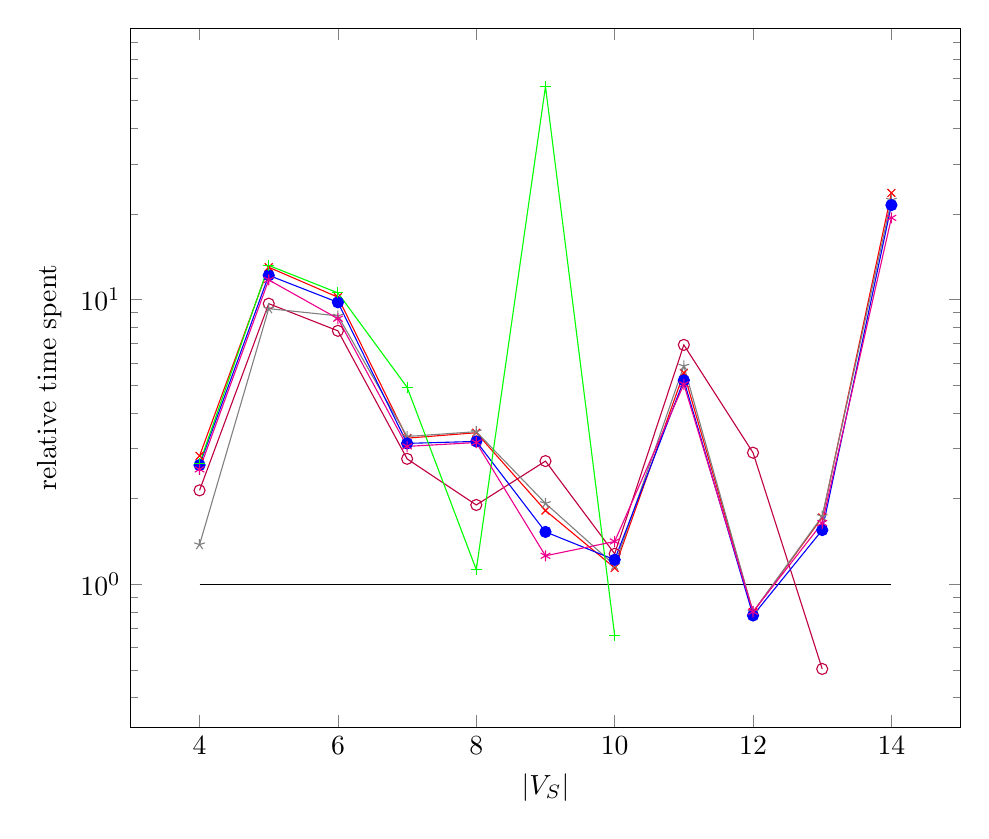
\begin{tikzpicture}
    \begin{axis}[
        xlabel=$|V_S|$,
        ylabel=relative time spent,
        ymode=log,
        legend style={at={(0.9,0.1)},anchor=south east},
        width=\textwidth,
		y tick label style={/pgf/number format/sci},
    ]
\addplot [mark=none, black] plot coordinates {
        (4,1) (14, 1)};





\addplot[
        mark=x,
        red,
    ] plot coordinates {
        (4,2.8251795368790886)
        (5,12.999580346656751)
        (6,10.202174684933484)
        (7,3.262604211259584)
        (8,3.408918438863976)
        (9,1.8166545299203807)
        (10,1.1422160886456934)
        (11,5.530516473257274)
        (12,0.7986133987525276)
        (13,1.7180491450318693)
        (14,23.721522460227753)
};
%    \addlegendentry{DFS}
\addplot[
        mark=o,
        purple,
    ] plot coordinates {
        (4,2.1391785196119923)
        (5,9.683057001857964)
        (6,7.773825041515071)
        (7,2.7604466990768595)
        (8,1.9008757163878494)
        (9,2.7101513865191915)
        (10,1.2805148059566114)
        (11,6.937603075441524)
        (12,2.9004853202789205)
        (13,0.5045390730335063)
};
%    \addlegendentry{GDFS O IP}


\addplot[
        mark=star,
        gray,
    ] plot coordinates {
        (4,1.3794140730076914)
        (5,9.299733094390856)
        (6,8.772951593738188)
        (7,3.307376496667975)
        (8,3.4383266889141892)
        (9,1.9254251970590692)
        (10,1.1671557982423402)
        (11,5.851599859841392)
        (12,0.7997588706522294)
        (13,1.7348281924961175)
        (14,22.40100510075956)
};
%    \addlegendentry{GDFS C}


\addplot[
        mark=*,
        blue,
    ] plot coordinates {
        (4,2.6239880026319113)
        (5,12.176055240511092)
        (6,9.786244499035096)
        (7,3.127359936505137)
        (8,3.1774880567968005)
        (9,1.528458868204552)
        (10,1.2199898778953424)
        (11,5.209122239775357)
        (12,0.7776618244283469)
        (13,1.5513809856510496)
        (14,21.49466036911607)
};
%    \addlegendentry{K-Path}


\addplot[
        mark=+,
        green,
    ] plot coordinates {
        (4,2.6615145962479296)
        (5,13.192185281822104)
        (6,10.56726292801845)
        (7,4.92388122723026)
        (8,1.126596319598566)
        (9,56.0969304160683)
        (10,0.6621016861467689)
};
%    \addlegendentry{CP}


\addplot[
        mark=asterisk,
        magenta,
    ] plot coordinates {
        (4,2.5345706323293955)
        (5,11.732948804586153)
        (6,8.577253069471816)
        (7,3.052311500224188)
        (8,3.1492268511393373)
        (9,1.2598729843415928)
        (10,1.414481795839197)
        (11,5.042048634623404)
        (12,0.8013450614402682)
        (13,1.642270880020916)
        (14,19.386486921496203)
};
%    \addlegendentry{GDFS A IP}



	
    \end{axis}
    \end{tikzpicture}

\caption{cached 1.5}
\label{fig:sub2}
\end{subfigure}
}
\newline
\resizebox{0.28\textheight}{!}{
\begin{subfigure}{0.5\linewidth}

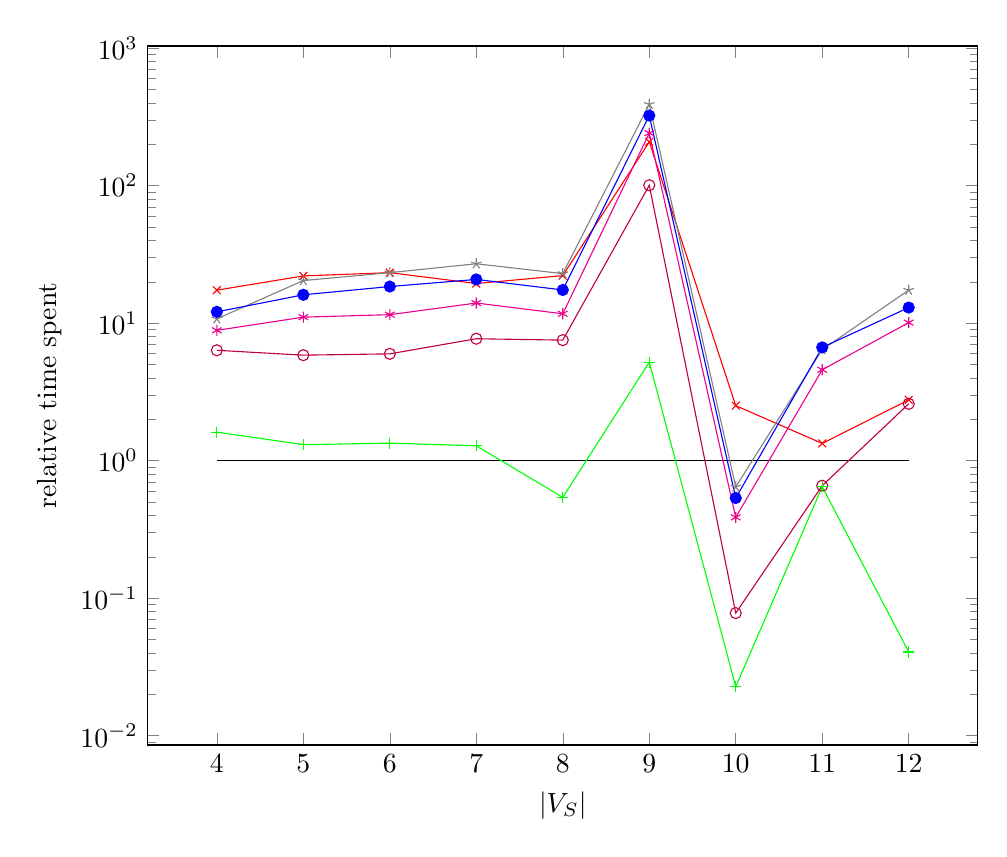
\begin{tikzpicture}
    \begin{axis}[
        xlabel=$|V_S|$,
        ylabel=relative time spent,
        ymode=log,
        legend style={at={(0.9,0.1)},anchor=south east},
        width=\textwidth,
		y tick label style={/pgf/number format/sci},
    ]
\addplot [mark=none, black] plot coordinates {
        (4,1) (12, 1)};
        
%    \node[] at (axis cs: 9,1.1) {Awaiting test results (CAES server)};


\addplot[
        mark=x,
        red,
    ] plot coordinates {
        (4,17.386687830540524)
        (5,22.079291788970327)
        (6,23.306743149976228)
        (7,19.430501058064742)
        (8,22.18188165942091)
        (9,208.2138028355397)
        (10,2.513700580968542)
        (11,1.3354403700554096)
        (12,2.769685497589875)
};
%    \addlegendentry{DFS}


\addplot[
        mark=o,
        purple,
    ] plot coordinates {
        (4,6.352134028283731)
        (5,5.854587074510253)
        (6,5.985860240907849)
        (7,7.709398766817202)
        (8,7.530947931423977)
        (9,100.71864029454015)
        (10,0.07798933813487574)
        (11,0.6582569130981772)
        (12,2.5920862258520847)
};
%    \addlegendentry{GDFS O IP}
\addplot[
        mark=star,
        gray,
    ] plot coordinates {
        (4,10.761013649646893)
        (5,20.41574344572187)
        (6,23.304616084965065)
        (7,27.046121301467018)
        (8,22.92486770453236)
        (9,390.8923046050332)
        (10,0.6451925167117611)
        (11,6.426992380187482)
        (12,17.397334287179326)
};
%    \addlegendentry{GDFS C}


\addplot[
        mark=*,
        blue,
    ] plot coordinates {
        (4,12.096262623777024)
        (5,16.08617175919)
        (6,18.475144819368374)
        (7,20.81253092789625)
        (8,17.4435299319244)
        (9,323.5049321924643)
        (10,0.5356093481057399)
        (11,6.667174509238782)
        (12,12.992684943846735)
};
%    \addlegendentry{K-Path}


\addplot[
        mark=+,
        green,
    ] plot coordinates {
        (4,1.6139175990246586)
        (5,1.308680553430318)
        (6,1.3420234704630691)
        (7,1.2831364418331979)
        (8,0.5413740631720213)
        (9,5.2062116151636655)
        (10,0.02272540669855816)
        (11,0.646307333488348)
        (12,0.04065603348894453)
};
%    \addlegendentry{CP}


\addplot[
        mark=asterisk,
        magenta,
    ] plot coordinates {
        (4,8.870187999266555)
        (5,11.06879290067633)
        (6,11.530569519342539)
        (7,14.018534191414552)
        (8,11.707182654942214)
        (9,240.92574467452093)
        (10,0.3875006668882859)
        (11,4.588294705762263)
        (12,10.093545772616306)
};
%    \addlegendentry{GDFS A IP}


    \end{axis}
    \end{tikzpicture}

\caption{uncached 3.0}
\label{fig:sub3}
\end{subfigure}
}
\resizebox{0.28\textheight}{!}{
\begin{subfigure} {0.5\linewidth}

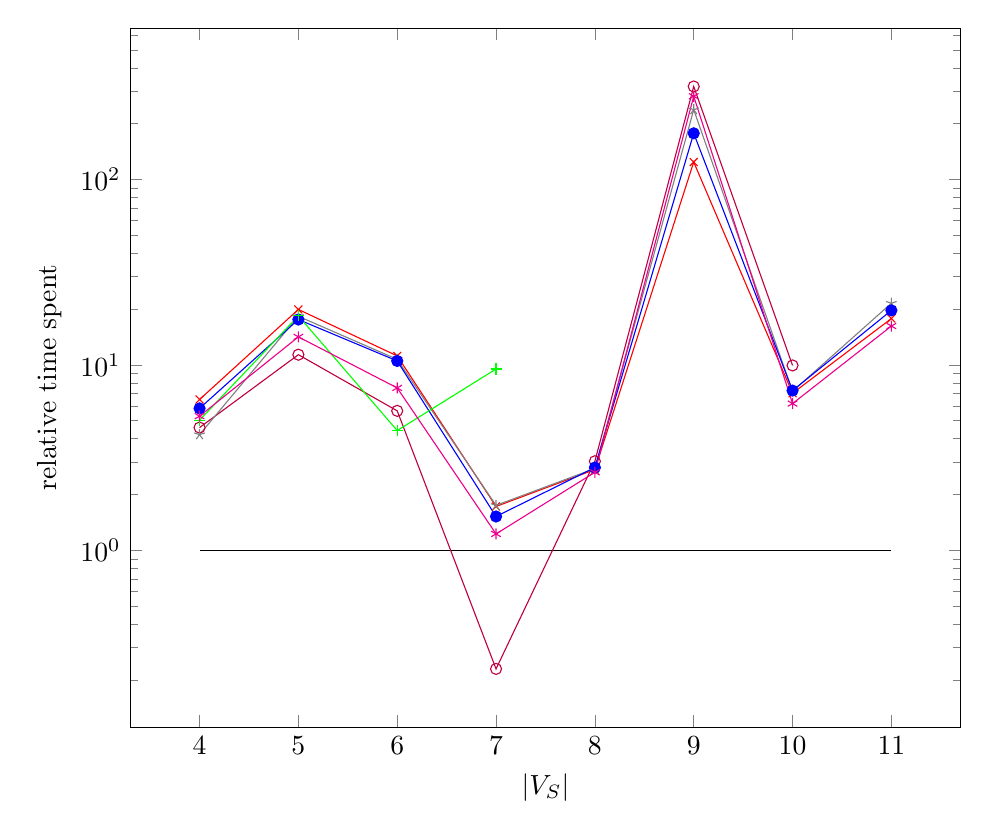
\begin{tikzpicture}
    \begin{axis}[
        xlabel=$|V_S|$,
        ylabel=relative time spent,
        ymode=log,
        legend style={at={(0.9,0.1)},anchor=south east},
        width=\textwidth,
		y tick label style={/pgf/number format/sci},
    ]
\addplot [mark=none, black] plot coordinates {
        (4,1) (11, 1)};

%    \node[] at (axis cs: 9,1.1) {Awaiting test results (CAES server)};


\addplot[
        mark=x,
        red,
    ] plot coordinates {
        (4,6.506721650403205)
        (5,19.909363887543122)
        (6,11.177297154921606)
        (7,1.724519080351556)
        (8,2.7285266745194945)
        (9,124.16181657015836)
        (10,7.031445004959032)
        (11,17.775679517060333)
};
%    \addlegendentry{DFS}


\addplot[
        mark=o,
        purple,
    ] plot coordinates {
        (4,4.591167743768188)
        (5,11.350912752822408)
        (6,5.65138232112045)
        (7,0.22941169442122966)
        (8,3.022521866223289)
        (9,317.2200653821222)
        (10,9.933613641908536)
};
%    \addlegendentry{GDFS O IP}


\addplot[
        mark=star,
        gray,
    ] plot coordinates {
        (4,4.207074680497982)
        (5,18.284434265485746)
        (6,10.709129649746266)
        (7,1.7482843191894677)
        (8,2.7628381393187915)
        (9,237.7691906661526)
        (10,7.2060962391545695)
        (11,21.510504634766995)
};
%    \addlegendentry{GDFS C}


\addplot[
        mark=*,
        blue,
    ] plot coordinates {
        (4,5.828596980071678)
        (5,17.56552393240703)
        (6,10.500132546594331)
        (7,1.5222497146218434)
        (8,2.7964449321329083)
        (9,177.3520386845159)
        (10,7.269881235493629)
        (11,19.678511605024486)
};
%    \addlegendentry{K-Path}
\addplot[
        mark=+,
        green,
    ] plot coordinates {
        (4,5.034988757242889)
        (5,18.379644895855858)
        (6,4.42492369951899)
        (7,9.504410596005838)
};
%    \addlegendentry{CP}


\addplot[
        mark=asterisk,
        magenta,
    ] plot coordinates {
        (4,5.291688590357283)
        (5,14.16162037925404)
        (6,7.513687814173463)
        (7,1.2262338445252592)
        (8,2.635480706053349)
        (9,280.95194542270235)
        (10,6.186575229718758)
        (11,16.197435578006964)
};
%    \addlegendentry{GDFS A IP}


	
    \end{axis}
    \end{tikzpicture}
    \caption{cached 3.0}

\end{subfigure}
}
\newline
\resizebox{0.28\textheight}{!}{
\begin{subfigure} {0.5\linewidth}

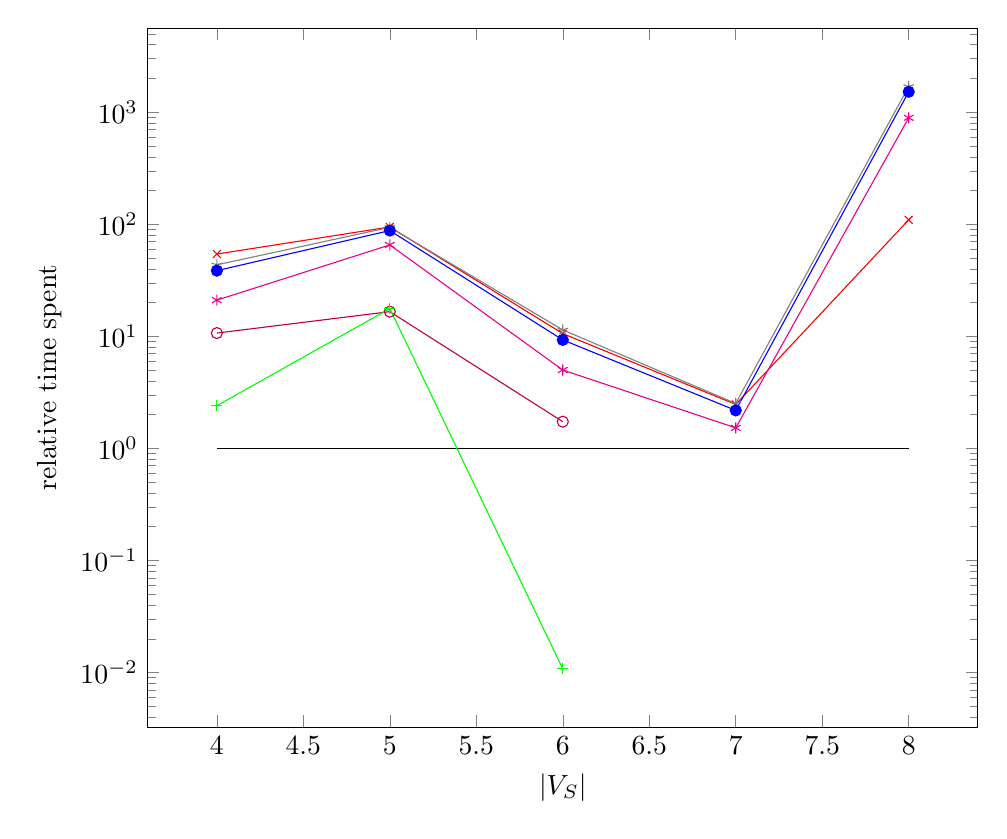
\begin{tikzpicture}
    \begin{axis}[
        xlabel=$|V_S|$,
        ylabel=relative time spent,
        ymode=log,
        legend style={at={(0.9,0.1)},anchor=south east},
        width=\textwidth,
		y tick label style={/pgf/number format/sci},
    ]
\addplot [mark=none, black] plot coordinates {
        (4,1) (8, 1)};


%    \node[] at (axis cs: 9,1.1) {Awaiting test results (CAES server)};


\addplot[
        mark=x,
        red,
    ] plot coordinates {
        (4,54.244632157024924)
        (5,94.67410125160248)
        (6,10.579022919199833)
        (7,2.467884806621709)
        (8,109.61796961417762)
};
%    \addlegendentry{DFS}
\addplot[
        mark=o,
        purple,
    ] plot coordinates {
        (4,10.696848569213739)
        (5,16.61647755676102)
        (6,1.7322365504694384)
};
%    \addlegendentry{GDFS O IP}


\addplot[
        mark=star,
        gray,
    ] plot coordinates {
        (4,43.465930808198564)
        (5,93.92255198591933)
        (6,11.412954212374762)
        (7,2.518522472050785)
        (8,1697.6384316902834)
};
%    \addlegendentry{GDFS C}


\addplot[
        mark=*,
        blue,
    ] plot coordinates {
        (4,38.576420798557756)
        (5,87.89857301021381)
        (6,9.292817526299109)
        (7,2.183982399647286)
        (8,1521.5144724464335)
};
%    \addlegendentry{K-Path}


\addplot[
        mark=+,
        green,
    ] plot coordinates {
        (4,2.4051156279390042)
        (5,17.69226975418839)
        (6,0.01077006183520568)
};
%    \addlegendentry{CP}


\addplot[
        mark=asterisk,
        magenta,
    ] plot coordinates {
        (4,21.03540301694324)
        (5,65.43192659713577)
        (6,5.008411731723122)
        (7,1.525357905120218)
        (8,892.0214429471364)
};
%    \addlegendentry{GDFS A IP}


	
    \end{axis}
    \end{tikzpicture}
    \caption{uncached 5.0}

\end{subfigure}
}
\resizebox{0.28\textheight}{!}{
\begin{subfigure} {0.5\linewidth}

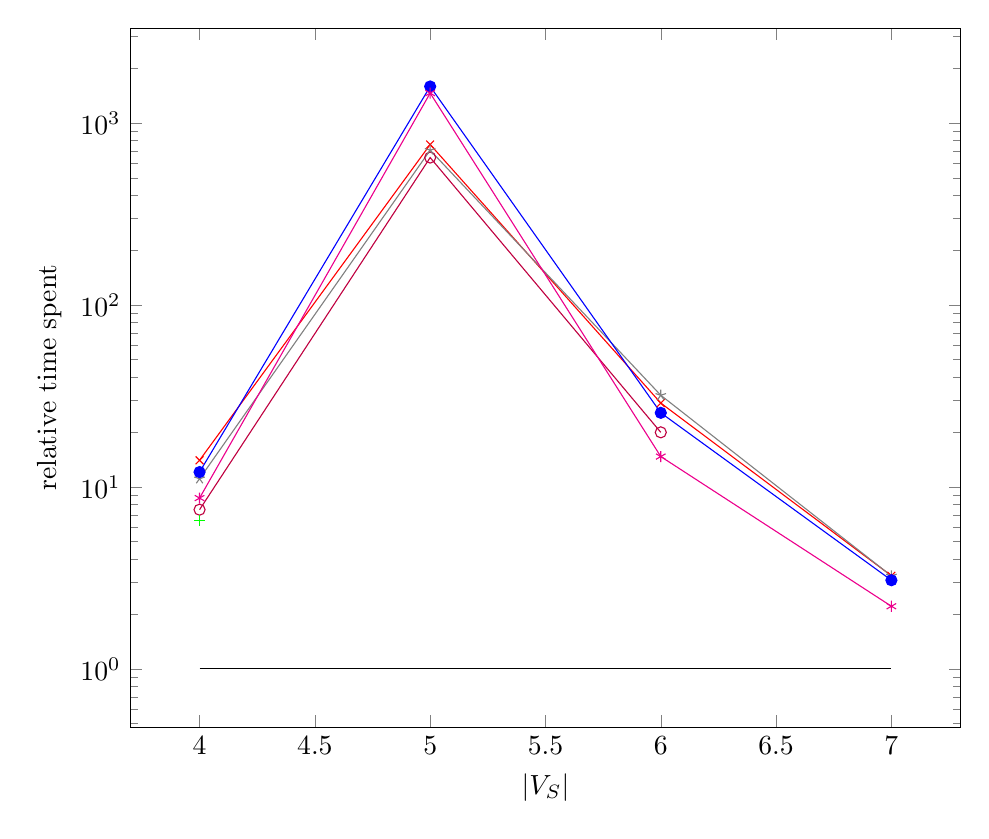
\begin{tikzpicture}
    \begin{axis}[
        xlabel=$|V_S|$,
        ylabel=relative time spent,
        ymode=log,
        legend style={at={(0.9,0.1)},anchor=south east},
        width=\textwidth,
		y tick label style={/pgf/number format/sci},
    ]
\addplot [mark=none, black] plot coordinates {
        (4,1) (7, 1)};

%    \node[] at (axis cs: 9,1.1) {Awaiting test results (CAES server)};


\addplot[
        mark=x,
        red,
    ] plot coordinates {
        (4,14.014442936425434)
        (5,762.1422676420387)
        (6,28.909066998258137)
        (7,3.2500045042967773)
};
%    \addlegendentry{DFS}


\addplot[
        mark=o,
        purple,
    ] plot coordinates {
        (4,7.500984134455194)
        (5,645.9950612990576)
        (6,19.964026565489586)
};
%    \addlegendentry{GDFS O IP}


\addplot[
        mark=star,
        gray,
    ] plot coordinates {
        (4,11.095723351464535)
        (5,709.242281166574)
        (6,31.912378240077096)
        (7,3.2455637430524833)
};
%    \addlegendentry{GDFS C}


\addplot[
        mark=*,
        blue,
    ] plot coordinates {
        (4,12.071862186804472)
        (5,1588.441230780402)
        (6,25.547353262290816)
        (7,3.0715704037334586)
};
%    \addlegendentry{K-Path}
\addplot[
        mark=+,
        green,
    ] plot coordinates {
        (4,6.572698252534947)
};
%    \addlegendentry{CP}


\addplot[
        mark=asterisk,
        magenta,
    ] plot coordinates {
        (4,8.686387496374607)
        (5,1460.2833829253511)
        (6,14.692897155453814)
        (7,2.2099232478638378)
};
%    \addlegendentry{GDFS A IP}


	
    \end{axis}
    \end{tikzpicture}
    \caption{cached 5.0}

\end{subfigure}
}

\caption{Performance of our algorithm with the distance based target graph vertex order relative to the performance of the algorithm with the degree-based target graph vertex order. We avoid unnecessarily long paths, do not perform contraction and use no pruning. Data points above the black reference line denote that this ordering introduces more delay, and data points below the reference line denote that this ordering saves time. Note the logarithmic y-axis.}		
\label{fig:DistanceVersusDegree}
\end{figure}



\begin{figure}
\begin{subfigure}{.5\linewidth}
\centering

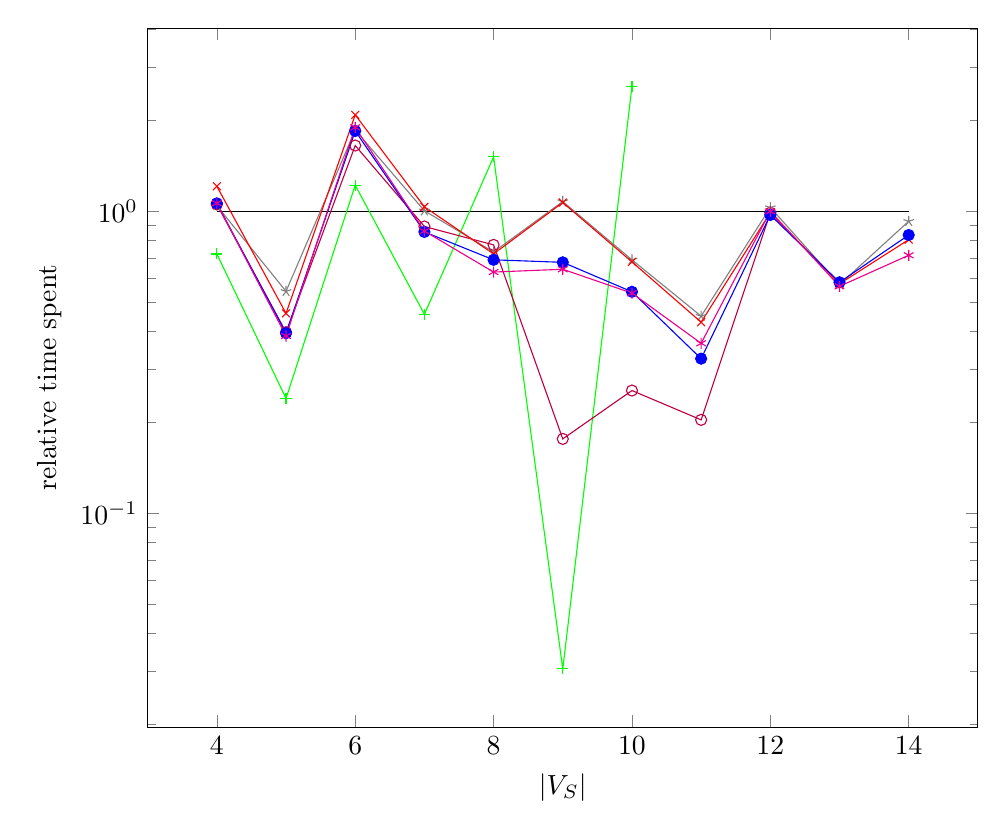
\begin{tikzpicture}
    \begin{axis}[
        xlabel=$|V_S|$,
        ylabel=relative time spent,
        ymode=log,
        legend style={at={(0.9,0.1)},anchor=south east},
        width=\textwidth,
		y tick label style={/pgf/number format/sci},
    ]


\addplot [mark=none, black] plot coordinates {
        (4,1) (14, 1)};
%\addlegendentry{No contraction}

\addplot[
        mark=+,
        green,
    ] plot coordinates {
        (4,0.7216233008103387)
        (5,0.23979959256395095)
        (6,1.219055373815801)
        (7,0.45549808099886696)
        (8,1.5129803175671477)
        (9,0.030491817239336187)
        (10,2.587109386205813)
};
%    \addlegendentry{CP}

\addplot[
        mark=o,
        purple,
    ] plot coordinates {
        (4,1.0524711376958586)
        (5,0.397430142997267)
        (6,1.649483210945216)
        (7,0.8895236575282935)
        (8,0.7731988158571639)
        (9,0.17613609063915775)
        (10,0.25469552245651866)
        (11,0.20364401173813004)
        (12,0.9888612062339083)
};
%    \addlegendentry{GDFS O IP}

\addplot[
        mark=star,
        gray,
    ] plot coordinates {
        (4,1.0424825365257937)
        (5,0.5426295402334718)
        (6,1.855682646836014)
        (7,1.0030303685825734)
        (8,0.732541042585068)
        (9,1.0760282051348324)
        (10,0.6898563436739937)
        (11,0.4490497012282625)
        (12,1.0279132116341756)
        (13,0.5714085857541255)
        (14,0.9256163980737115)
};
%    \addlegendentry{GDFS C}

\addplot[
        mark=x,
        red,
    ] plot coordinates {
        (4,1.208819655001192)
        (5,0.4586488473969574)
        (6,2.083424951258273)
        (7,1.0333509881095415)
        (8,0.7217323256161471)
        (9,1.067791165771744)
        (10,0.6792053743658721)
        (11,0.42883471023577835)
        (12,0.9888018890272706)
        (13,0.5747328589505348)
        (14,0.8046705504898993)
};
%    \addlegendentry{DFS}

\addplot[
        mark=*,
        blue,
    ] plot coordinates {
        (4,1.0612749917741098)
        (5,0.3945236842140588)
        (6,1.8429590288918432)
        (7,0.8535961630308873)
        (8,0.6899304068674341)
        (9,0.6769900545914925)
        (10,0.5407198063482145)
        (11,0.3247299866242016)
        (12,0.9713817184344807)
        (13,0.5813925975914811)
        (14,0.8336248540971392)
};
%    \addlegendentry{K-Path}

\addplot[
        mark=asterisk,
        magenta,
    ] plot coordinates {
        (4,1.0622283595408073)
        (5,0.38615187683924507)
        (6,1.894044220650229)
        (7,0.8590163375653131)
        (8,0.6286080587791637)
        (9,0.6420560054284833)
        (10,0.5352470679476732)
        (11,0.36511431500997044)
        (12,0.9985286266608072)
        (13,0.5638366376132966)
        (14,0.7142330269028185)
};
%    \addlegendentry{GDFS A IP}




    \end{axis}
    \end{tikzpicture}


\caption{$|V_T|=1\frac{1}{2}|V_S|$}
\label{fig:sub1}
\end{subfigure}%
\begin{subfigure}{.5\linewidth}
\centering

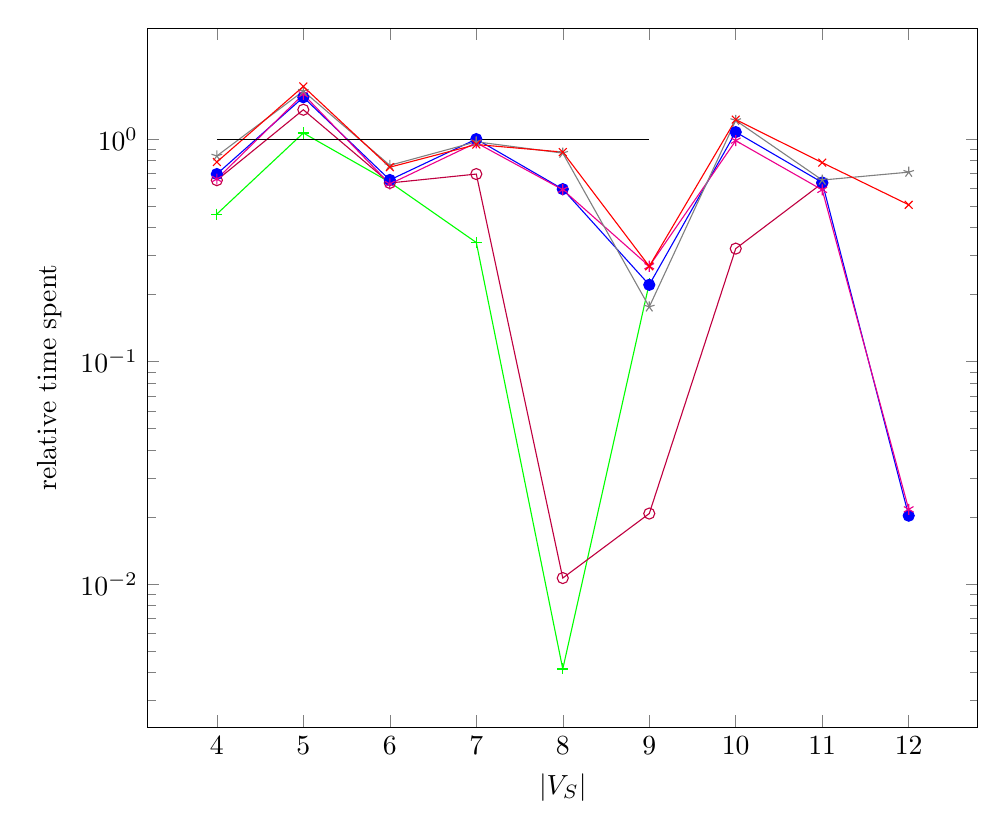
\begin{tikzpicture}
    \begin{axis}[
        xlabel=$|V_S|$,
        ylabel=relative time spent,
        ymode=log,
        legend style={at={(0.9,0.1)},anchor=south east},
        width=\textwidth,
		y tick label style={/pgf/number format/sci},
    ]

\addplot[
        mark=+,
        green,
    ] plot coordinates {
        (4,0.4603454215293834)
        (5,1.0650216337194074)
        (6,0.6402609902641055)
        (7,0.3429545951232229)
        (8,0.004156976828625529)
        (9,0.22489814118245785)
};
 %   \addlegendentry{CP}
    
    \addplot[
        mark=o,
        purple,
    ] plot coordinates {
        (4,0.6536194606761304)
        (5,1.3546625727069868)
        (6,0.6349737425008939)
        (7,0.6963677891889153)
        (8,0.010649285020911963)
        (9,0.02075639387474258)
        (10,0.3219692946843138)
        (11,0.6331864854788115)
};
 %   \addlegendentry{GDFS O IP}

\addplot[
        mark=*,
        blue,
    ] plot coordinates {
        (4,0.6964763815520504)
        (5,1.5418767352722276)
        (6,0.655132639298351)
        (7,0.9999288333397025)
        (8,0.5958121258705841)
        (9,0.22131003316388181)
        (10,1.0751746486592535)
        (11,0.6382538165641153)
        (12,0.02029968985193284)
};
  %  \addlegendentry{K-Path}
    
    
    \addplot[
        mark=asterisk,
        magenta,
    ] plot coordinates {
        (4,0.6613792478641376)
        (5,1.5903154443877043)
        (6,0.6283278818175081)
        (7,0.9629244885375634)
        (8,0.5921232096268492)
        (9,0.2682914762370498)
        (10,0.9835719984313271)
        (11,0.5912237044773625)
        (12,0.02168235616079701)
};
  %  \addlegendentry{GDFS A IP}
    
    
    \addplot[
        mark=star,
        gray,
    ] plot coordinates {
        (4,0.8400238494760311)
        (5,1.6432913297339495)
        (6,0.7623783834679656)
        (7,0.9724418464068187)
        (8,0.8649452249859358)
        (9,0.17617155505832582)
        (10,1.212740370430325)
        (11,0.6545125286561274)
        (12,0.7102484891877338)
};
 %   \addlegendentry{GDFS C}
    
    \addplot[
        mark=x,
        red,
    ] plot coordinates {
        (4,0.7890817980923504)
        (5,1.7236983707312352)
        (6,0.7476536478460998)
        (7,0.9454835701186506)
        (8,0.8743040069418077)
        (9,0.2682189465805335)
        (10,1.2231897365346933)
        (11,0.7838936485791846)
        (12,0.5066592201432429)
};
%    \addlegendentry{DFS}

\addplot [mark=none, black] plot coordinates {
        (4,1) (9, 1)};
%\addlegendentry{No contraction}


	
    \end{axis}
    \end{tikzpicture}

\caption{$|V_T|=3|V_S|$}
\label{fig:sub2}
\end{subfigure}\\[1ex]
\begin{subfigure}{0.5\linewidth}
\centering

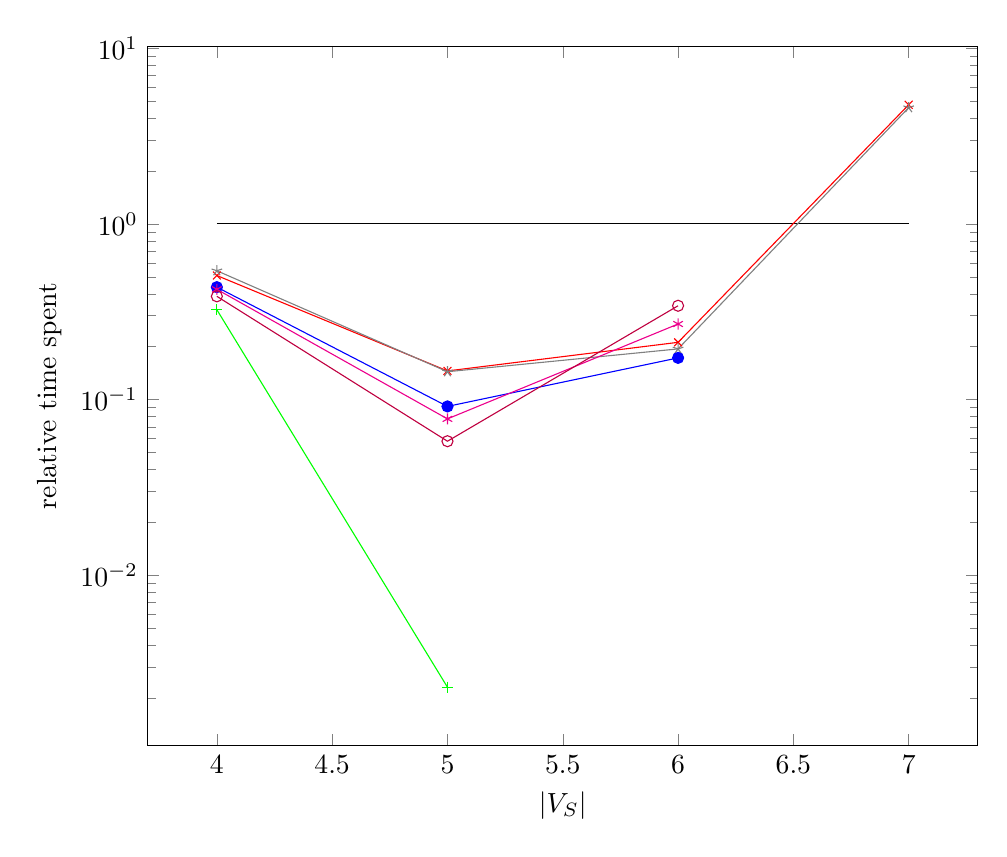
\begin{tikzpicture}
    \begin{axis}[
        xlabel=$|V_S|$,
        ylabel=relative time spent,
        ymode=log,
        legend style={at={(0.9,0.1)},anchor=south east},
        width=\textwidth,
		y tick label style={/pgf/number format/sci},
    ]


\addplot [mark=none, black] plot coordinates {
        (4,1) (7, 1)};
%\addlegendentry{No contraction}
\addplot[
        mark=+,
        green,
    ] plot coordinates {
        (4,0.3247986778213492)
        (5,0.0023085173636887735)
};
%    \addlegendentry{CP}


\addplot[
        mark=x,
        red,
    ] plot coordinates {
        (4,0.5083088516623958)
        (5,0.14560631066960938)
        (6,0.21180693936992814)
        (7,4.763971312568752)
};
 %   \addlegendentry{DFS}


\addplot[
        mark=star,
        gray,
    ] plot coordinates {
        (4,0.5412364762939754)
        (5,0.14410181776854825)
        (6,0.19432561438404647)
        (7,4.587173792533694)
};
%    \addlegendentry{GDFS C}


\addplot[
        mark=*,
        blue,
    ] plot coordinates {
        (4,0.43647426849988535)
        (5,0.09146773493441722)
        (6,0.17275569282732595)
};
 %   \addlegendentry{K-Path}


\addplot[
        mark=asterisk,
        magenta,
    ] plot coordinates {
        (4,0.4241962520645475)
        (5,0.07767539614505417)
        (6,0.26930850582566696)
};
 %   \addlegendentry{GDFS A IP}


\addplot[
        mark=o,
        purple,
    ] plot coordinates {
        (4,0.38706533483340066)
        (5,0.05797333316929685)
        (6,0.34203860563242006)
};
%    \addlegendentry{GDFS O IP}

	
	
    \end{axis}
    \end{tikzpicture}

\caption{$|V_T|=5|V_S|$}
\label{fig:sub3}
\end{subfigure}
\begin{subfigure} {0.5\linewidth}
\centering

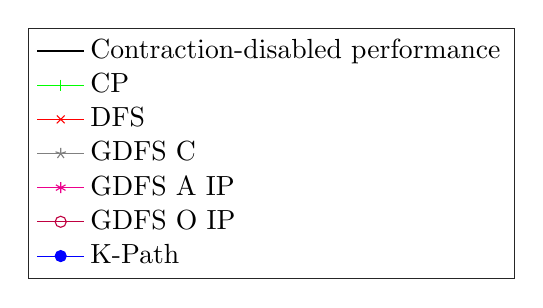
\begin{tikzpicture} 
    \begin{axis}[%
    hide axis,
    xmin=10,
    xmax=50,
    ymin=0,
    ymax=0.4,
    legend style={draw=white!15!black,legend cell align=left}
    ]
	\addlegendimage{black}
    \addlegendentry{Contraction-disabled performance}; 
     
    \addlegendimage{green, mark=+}
    \addlegendentry{CP};
    
    \addlegendimage{red, mark=x}
    \addlegendentry{DFS};
    
    \addlegendimage{gray, mark=star}
    \addlegendentry{GDFS C};
    
    \addlegendimage{magenta, mark=asterisk}
    \addlegendentry{GDFS A IP};
    
    \addlegendimage{purple, mark=o}
    \addlegendentry{GDFS O IP};
    
    \addlegendimage{blue, mark=*}
    \addlegendentry{K-Path};
    
    \end{axis}
\end{tikzpicture}

\end{subfigure}

\caption{Performance of our algorithm with the degree-based target graph vertex order relative to the performance of the algorithm with a random target graph vertex order. We avoid unnecessarily long paths, do not perform contraction and use no pruning. Data points above the black reference line denote the degree-based ordering introduces more delay, and data points below the reference line denote that it saves time. Note the logarithmic y-axis.}	
\label{fig:greatestDegreeVersusRandom}
\end{figure}



\begin{figure}
\begin{subfigure}{.5\linewidth}
\centering

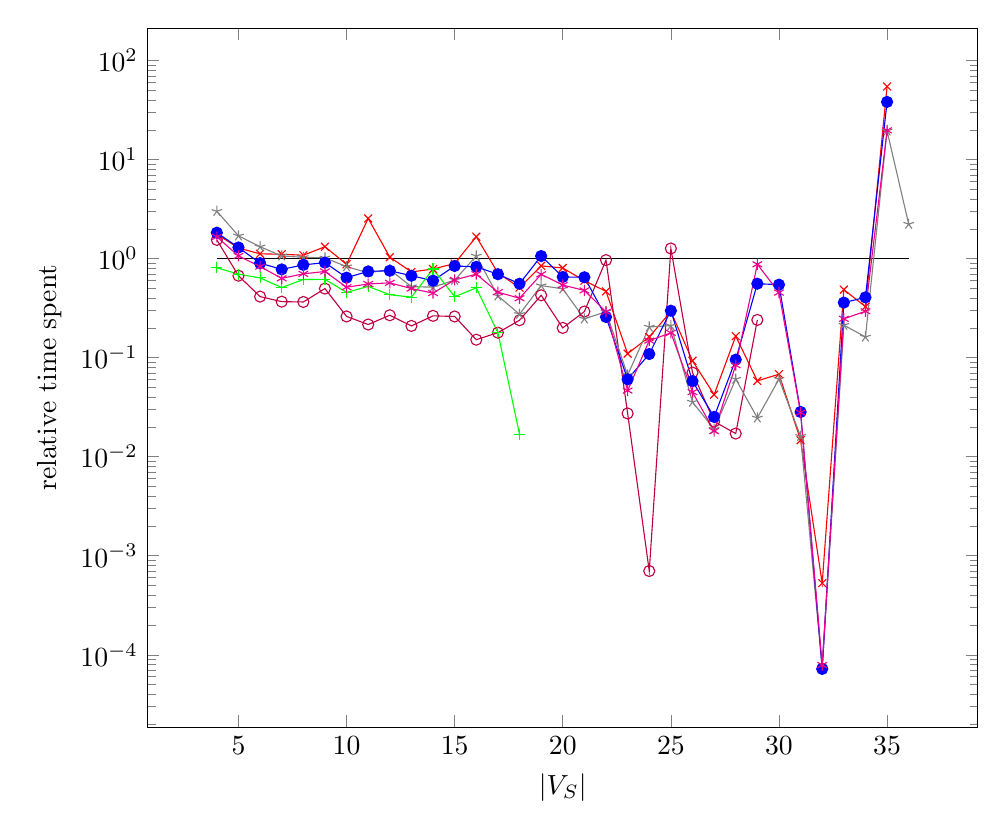
\begin{tikzpicture}
    \begin{axis}[
        xlabel=$|V_S|$,
        ylabel=relative time spent,
        ymode=log,
        legend style={at={(0.9,0.1)},anchor=south east},
        width=\textwidth,
		y tick label style={/pgf/number format/sci},
    ]


\addplot [mark=none, black] plot coordinates {
        (4,1) (36, 1)};
%\addlegendentry{No contraction}

	
    \addplot[
        mark=x,
        red,
    ] plot coordinates {
        (4,1.764570104072358)
        (5,1.2804472403537654)
        (6,1.1184611822085426)
        (7,1.108193754987779)
        (8,1.0823455102636332)
        (9,1.3202304844536292)
        (10,0.8766301350767352)
        (11,2.545919815002013)
        (12,1.0352805568707166)
        (13,0.7348584756068407)
        (14,0.7849914287368015)
        (15,0.8934474568976407)
        (16,1.6666025961560895)
        (17,0.71724791351521)
        (18,0.5094398225741126)
        (19,0.8456597164761079)
        (20,0.8045735438552715)
        (21,0.5994679253970462)
        (22,0.4676165222586781)
        (23,0.10986432258137258)
        (24,0.16189794326161777)
        (25,0.2926263173443996)
        (26,0.09304326805518515)
        (27,0.042335345258718515)
        (28,0.1650463503335008)
        (29,0.05828381864786569)
        (30,0.06816890123257702)
        (31,0.014702001658170927)
        (32,5.292125517369906E-4)
        (33,0.48658861405918064)
        (34,0.3275583732734606)
        (35,54.77402524625391)
};
%    \addlegendentry{DFS}



\addplot[
        mark=o,
        purple,
    ] plot coordinates {
        (4,1.5465954055848148)
        (5,0.6725582833953612)
        (6,0.4139609581308408)
        (7,0.36803303109353136)
        (8,0.36527194171296373)
        (9,0.49852548813528896)
        (10,0.26095750210484203)
        (11,0.21624262398197047)
        (12,0.26820633077466083)
        (13,0.20928330156141128)
        (14,0.26458447534228824)
        (15,0.2606750959815698)
        (16,0.1519838230882713)
        (17,0.17898927491143424)
        (18,0.2388521888406996)
        (19,0.4267188749902131)
        (20,0.19982250009097213)
        (21,0.2924664720196809)
        (22,0.9672401778006531)
        (23,0.027360410960048376)
        (24,7.01509756650176E-4)
        (25,1.2672226912043596)
        (26,0.07078753406996308)
        (27,0.022665056711590914)
        (28,0.017141291453382168)
        (29,0.24055888434774642)
};
%    \addlegendentry{GDFS O IP}


    \addplot[
        mark=star,
        gray,
    ] plot coordinates {
        (4,3.0103172170217087)
        (5,1.7008010826730877)
        (6,1.3185993107748495)
        (7,1.0651222844937673)
        (8,1.0313582598355582)
        (9,1.019847433896466)
        (10,0.8297884970625686)
        (11,0.7200492247409158)
        (12,0.774512334885343)
        (13,0.5217949486742455)
        (14,0.5149663295021711)
        (15,0.6077016349543982)
        (16,1.0645804487651895)
        (17,0.4211041381764984)
        (18,0.2746875518186591)
        (19,0.5346278517377602)
        (20,0.4954917433705648)
        (21,0.24700068708986667)
        (22,0.2909598485628878)
        (23,0.06682556779896554)
        (24,0.20424256710140876)
        (25,0.2106670647954565)
        (26,0.035665701539059236)
        (27,0.018999300275658104)
        (28,0.06081303305299257)
        (29,0.02467804462419776)
        (30,0.06069641418283933)
        (31,0.016093817467386362)
        (32,7.397912089912584E-5)
        (33,0.21324629155751507)
        (34,0.1619915480935199)
        (35,19.49048948725945)
        (36,2.2331192579992156)
};
%    \addlegendentry{GDFS C}

    \addplot[
        mark=*,
        blue,
    ] plot coordinates {
        (4,1.8288452494372274)
        (5,1.296842120241007)
        (6,0.9012387818727957)
        (7,0.7791122372023914)
        (8,0.864968223092994)
        (9,0.911626513812194)
        (10,0.6427888393538057)
        (11,0.7436225584218299)
        (12,0.7549604979371962)
        (13,0.6725293793784693)
        (14,0.5992914625619475)
        (15,0.8435469822917079)
        (16,0.8272824596684006)
        (17,0.6960713562008894)
        (18,0.558150986832071)
        (19,1.0626322277949884)
        (20,0.6533296061774068)
        (21,0.6487638110734476)
        (22,0.2578033809500446)
        (23,0.06052594706960124)
        (24,0.10891268807752708)
        (25,0.2980748961720695)
        (26,0.05796008903103311)
        (27,0.025237959619589523)
        (28,0.09548260902564809)
        (29,0.5586781624508028)
        (30,0.5460070481456223)
        (31,0.02831601533804662)
        (32,7.199585374040307E-5)
        (33,0.3599020863720135)
        (34,0.40664654347704143)
        (35,38.25888474739304)
};
%    \addlegendentry{K-Path}
	\addplot[
        mark=+,
        green,
    ] plot coordinates {
        (4,0.8097147281048784)
        (5,0.6974807076483973)
        (6,0.6387765511195216)
        (7,0.5108136511953608)
        (8,0.6154822873000718)
        (9,0.6178076238665242)
        (10,0.4566675480771135)
        (11,0.5245224457353261)
        (12,0.43193355168311)
        (13,0.4090918564605406)
        (14,0.7867273649511707)
        (15,0.4132124817740861)
        (16,0.506998908675651)
        (17,0.17851266569571234)
        (18,0.016853231440474126)
};
%    \addlegendentry{CP}


    \addplot[
        mark=asterisk,
        magenta,
    ] plot coordinates {
        (4,1.6604963959561405)
        (5,1.0651196386902062)
        (6,0.8313893618484981)
        (7,0.6330831569415312)
        (8,0.7025851289861612)
        (9,0.7421127604924067)
        (10,0.5145838783545251)
        (11,0.555358976224104)
        (12,0.5695323766025293)
        (13,0.4990355735260106)
        (14,0.448887395328494)
        (15,0.6109556736209575)
        (16,0.6965392752667293)
        (17,0.4587395343719304)
        (18,0.3984597147505228)
        (19,0.6943628794563819)
        (20,0.5416331210064403)
        (21,0.47775841013253695)
        (22,0.29035493491769016)
        (23,0.04652391751293539)
        (24,0.14871288585077824)
        (25,0.1781947274150446)
        (26,0.04490122252456785)
        (27,0.018161498301854984)
        (28,0.08401938735395065)
        (29,0.8775983409797485)
        (30,0.4542658231858391)
        (31,0.027895820423659345)
        (32,7.878042538378427E-5)
        (33,0.2469129572361528)
        (34,0.2944533235188781)
        (35,19.738338899024424)
};
%    \addlegendentry{GDFS A IP}

    
   

    \end{axis}
    \end{tikzpicture}


\caption{$|V_T|=1\frac{1}{2}|V_S|$}
\label{fig:sub1}
\end{subfigure}%
\begin{subfigure}{.5\linewidth}
\centering

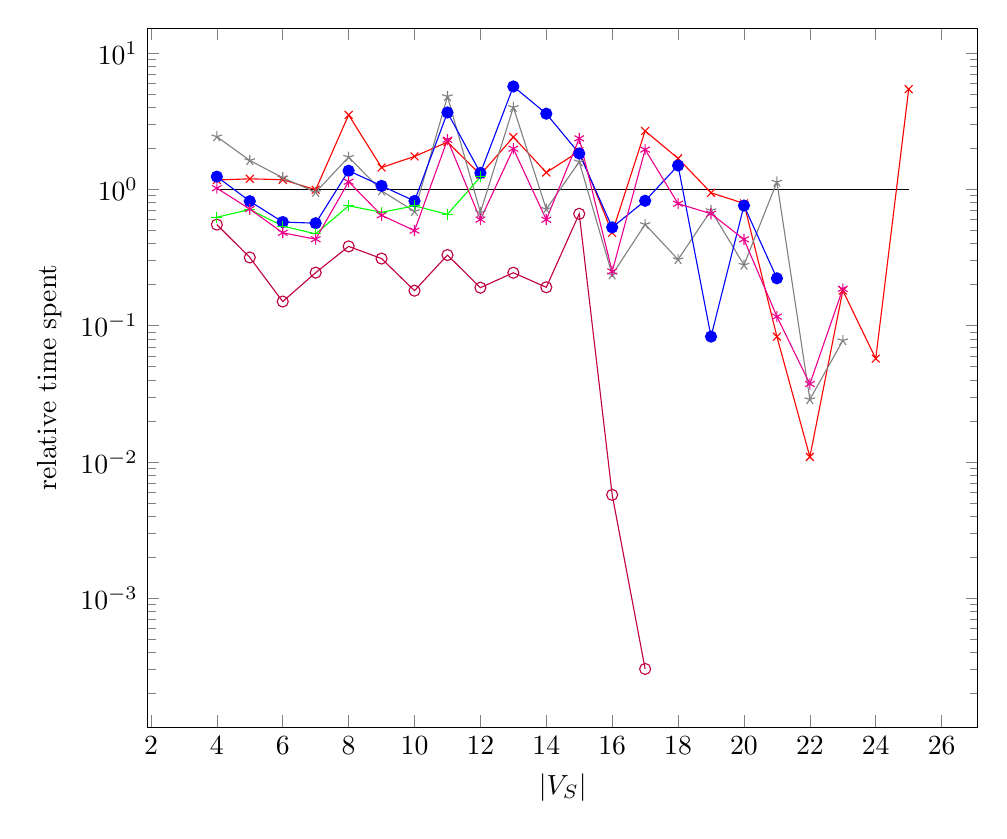
\begin{tikzpicture}
    \begin{axis}[
        xlabel=$|V_S|$,
        ylabel=relative time spent,
        ymode=log,
        legend style={at={(0.9,0.1)},anchor=south east},
        width=\textwidth,
		y tick label style={/pgf/number format/sci},
    ]


\addplot [mark=none, black] plot coordinates {
        (4,1) (25, 1)};
%\addlegendentry{No contraction}

	


\addplot[
        mark=x,
        red,
    ] plot coordinates {
        (4,1.1732605514536567)
        (5,1.196916188570318)
        (6,1.1785456812485087)
        (7,0.9954870013054639)
        (8,3.525437510655584)
        (9,1.4492110968852605)
        (10,1.747381055099775)
        (11,2.2270690506062127)
        (12,1.2853934585525963)
        (13,2.4238390071533145)
        (14,1.3323905497689534)
        (15,1.9053869795283003)
        (16,0.48107044214796724)
        (17,2.689105479333416)
        (18,1.6898544382126748)
        (19,0.9452484856043308)
        (20,0.7898504601171549)
        (21,0.08308472050964744)
        (22,0.010893076925442502)
        (23,0.1812527204673673)
        (24,0.05728059082927839)
        (25,5.443902225728544)
};
%    \addlegendentry{DFS}


\addplot[
        mark=o,
        purple,
    ] plot coordinates {
        (4,0.5520630930461605)
        (5,0.3167780166100581)
        (6,0.15039692039595431)
        (7,0.24510767406414147)
        (8,0.38213533186187054)
        (9,0.3108804215985045)
        (10,0.1807787773743944)
        (11,0.3299920410160406)
        (12,0.19012573181575232)
        (13,0.24472040784270033)
        (14,0.19143954341561553)
        (15,0.6627219343829152)
        (16,0.005733506512017317)
        (17,3.023867931706281E-4)
};
%    \addlegendentry{GDFS O IP}


\addplot[
        mark=star,
        gray,
    ] plot coordinates {
        (4,2.4400816563321017)
        (5,1.633197217665063)
        (6,1.2185290307235452)
        (7,0.9546648292258212)
        (8,1.728111058353678)
        (9,0.9769781523573012)
        (10,0.6904942121852058)
        (11,4.816564314417738)
        (12,0.6783371965634181)
        (13,4.011191995338261)
        (14,0.7170173730516766)
        (15,1.5965119303548203)
        (16,0.23663227697171496)
        (17,0.5542490660149222)
        (18,0.3058591166536577)
        (19,0.7018097729480665)
        (20,0.27875622792926213)
        (21,1.1344734954273632)
        (22,0.028755331201753886)
        (23,0.0777791424367319)
};
%    \addlegendentry{GDFS C}


\addplot[
        mark=*,
        blue,
    ] plot coordinates {
        (4,1.2419213216803755)
        (5,0.8200821368474451)
        (6,0.5765214516413038)
        (7,0.565346845113148)
        (8,1.3724712483006076)
        (9,1.0626551826303774)
        (10,0.8227740807006784)
        (11,3.6735922630894127)
        (12,1.3221239755232121)
        (13,5.700758822957509)
        (14,3.5989514748969498)
        (15,1.8366783161451987)
        (16,0.5267585376114875)
        (17,0.8256958007787268)
        (18,1.4987328025927649)
        (19,0.08315275360896346)
        (20,0.7615106824048338)
        (21,0.2227706812823126)
};
%    \addlegendentry{K-Path}
	\addplot[
        mark=+,
        green,
    ] plot coordinates {
        (4,0.6251754120590031)
        (5,0.7127354515628973)
        (6,0.5384995648933136)
        (7,0.4718614006762697)
        (8,0.7587386430883546)
        (9,0.6801119660951308)
        (10,0.7579067651040344)
        (11,0.6568766478712005)
        (12,1.2358097901656984)
};
%    \addlegendentry{CP}

\addplot[
        mark=asterisk,
        magenta,
    ] plot coordinates {
        (4,1.0218394225281529)
        (5,0.7182128970849538)
        (6,0.48051752660220404)
        (7,0.431379262711197)
        (8,1.139769610563402)
        (9,0.6462462777019891)
        (10,0.4984166569477635)
        (11,2.3191988060404114)
        (12,0.600719665743818)
        (13,1.9928831703649212)
        (14,0.5997476794608112)
        (15,2.3702852860015766)
        (16,0.2501718737108647)
        (17,1.963031760531809)
        (18,0.7865261017018875)
        (19,0.6636357792814185)
        (20,0.4302617051584967)
        (21,0.11666290941349455)
        (22,0.03731454564481351)
        (23,0.18654788991103444)
};
%    \addlegendentry{GDFS A IP}

	
	
    \end{axis}
    \end{tikzpicture}

\caption{$|V_T|=3|V_S|$}
\label{fig:sub2}
\end{subfigure}\\[1ex]
\begin{subfigure}{0.5\linewidth}
\centering

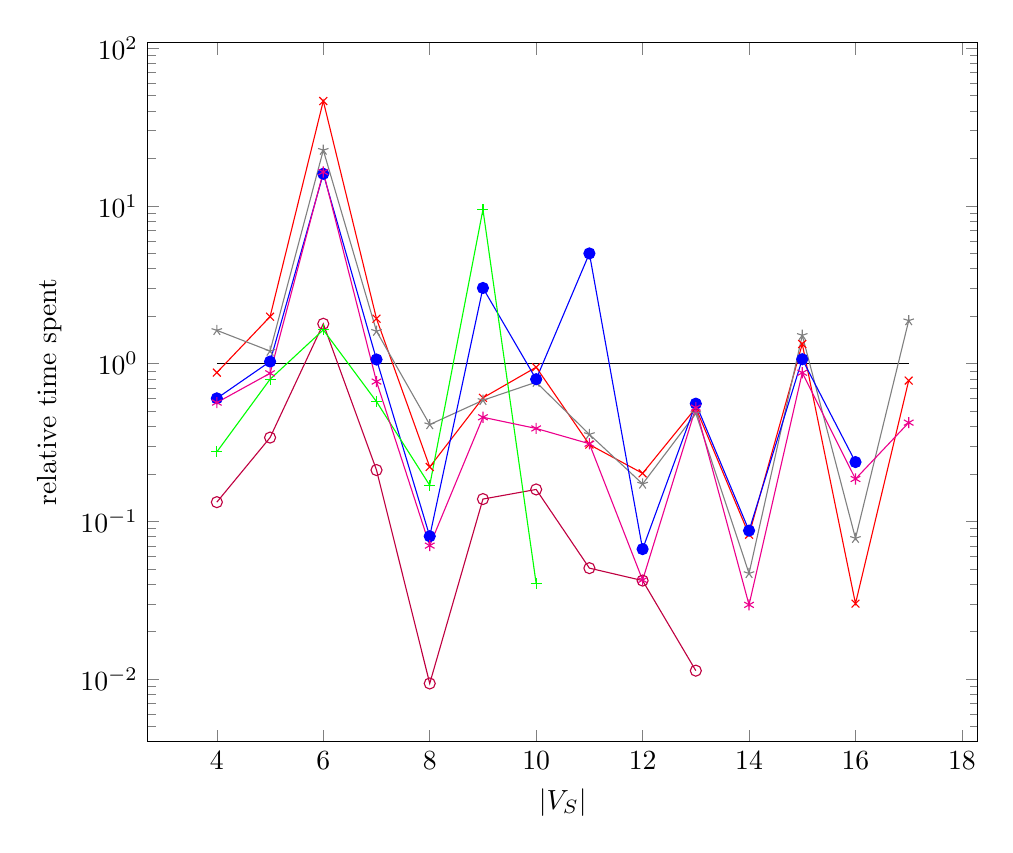
\begin{tikzpicture}
    \begin{axis}[
        xlabel=$|V_S|$,
        ylabel=relative time spent,
        ymode=log,
        legend style={at={(0.9,0.1)},anchor=south east},
        width=\textwidth,
		y tick label style={/pgf/number format/sci},
    ]


\addplot [mark=none, black] plot coordinates {
        (4,1) (17, 1)};
%\addlegendentry{No contraction}

	

  \addplot[
        mark=x,
        red,
    ] plot coordinates {
        (4,0.8783007924961822)
        (5,1.9866466250704127)
        (6,46.23915298831981)
        (7,1.9286013087935467)
        (8,0.22144887888388298)
        (9,0.6073880518853707)
        (10,0.9499470941285778)
        (11,0.3071513116204406)
        (12,0.20181763488775617)
        (13,0.5247142961355576)
        (14,0.08240035713162575)
        (15,1.3331646694970158)
        (16,0.030153907349204312)
        (17,0.7818188550294238)
};
%     \addlegendentry{DFS}

    \addplot[
        mark=o,
        purple,
    ] plot coordinates {
        (4,0.13253526170374963)
        (5,0.340135432164708)
        (6,1.790446045629151)
        (7,0.21172911942986739)
        (8,0.00939924729361108)
        (9,0.1386409264007632)
        (10,0.15954167221271842)
        (11,0.05059726207816495)
        (12,0.04218464066556149)
        (13,0.011328653011651979)
};
%    \addlegendentry{GDFS O IP}

 \addplot[
        mark=star,
        gray,
    ] plot coordinates {
        (4,1.6271054568492918)
        (5,1.2019347721569387)
        (6,22.57207288783596)
        (7,1.60714000055505)
        (8,0.41137411151774583)
        (9,0.5862167248296255)
        (10,0.7637400611154803)
        (11,0.356373039522627)
        (12,0.17288151392047257)
        (13,0.48433813085979627)
        (14,0.046838546665677216)
        (15,1.5140584943694408)
        (16,0.07823427303666675)
        (17,1.8750942580464485)
};
%    \addlegendentry{GDFS C}


\addplot[
        mark=*,
        blue,
    ] plot coordinates {
        (4,0.60298022841694)
        (5,1.0316944681766402)
        (6,15.991061194154563)
        (7,1.063190444555428)
        (8,0.08058508916228702)
        (9,3.019451686125926)
        (10,0.79704175618652)
        (11,4.998970774016183)
        (12,0.06678499576131569)
        (13,0.5580121902125518)
        (14,0.08746647794145956)
        (15,1.0672969432977613)
        (16,0.23788697499741307)
};
%    \addlegendentry{K-Path}

   \addplot[
        mark=+,
        green,
    ] plot coordinates {
        (4,0.2760410688096132)
        (5,0.7968662246398364)
        (6,1.6383115468640344)
        (7,0.5747225278886098)
        (8,0.16947067443329888)
        (9,9.48379348911334)
        (10,0.04037684393142793)
};
%    \addlegendentry{CP}
	\addplot[
        mark=asterisk,
        magenta,
    ] plot coordinates {
        (4,0.5669029018884123)
        (5,0.8690518164754274)
        (6,16.40156998152306)
        (7,0.7704428785494475)
        (8,0.07028167075789626)
        (9,0.4575408842013087)
        (10,0.38859339371640744)
        (11,0.31086090173433223)
        (12,0.0424840967267095)
        (13,0.5265194610065892)
        (14,0.02960328686421898)
        (15,0.8762590796270182)
        (16,0.1859213565027673)
        (17,0.42289838038406646)
};
%    \addlegendentry{GDFS A IP}

	
	
    \end{axis}
    \end{tikzpicture}

\caption{$|V_T|=5|V_S|$}
\label{fig:sub3}
\end{subfigure}
\begin{subfigure} {0.5\linewidth}
\centering

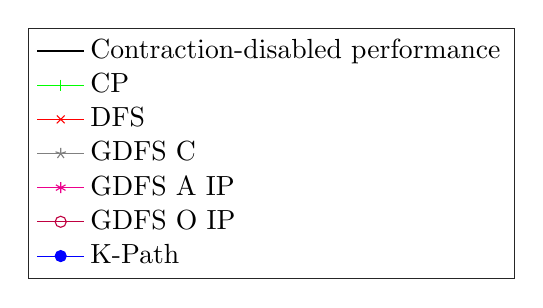
\begin{tikzpicture} 
    \begin{axis}[%
    hide axis,
    xmin=10,
    xmax=50,
    ymin=0,
    ymax=0.4,
    legend style={draw=white!15!black,legend cell align=left}
    ]
	\addlegendimage{black}
    \addlegendentry{Contraction-disabled performance}; 
     
    \addlegendimage{green, mark=+}
    \addlegendentry{CP};
    
    \addlegendimage{red, mark=x}
    \addlegendentry{DFS};
    
    \addlegendimage{gray, mark=star}
    \addlegendentry{GDFS C};
    
    \addlegendimage{magenta, mark=asterisk}
    \addlegendentry{GDFS A IP};
    
    \addlegendimage{purple, mark=o}
    \addlegendentry{GDFS O IP};
    
    \addlegendimage{blue, mark=*}
    \addlegendentry{K-Path};
    
    \end{axis}
\end{tikzpicture}

\end{subfigure}

\caption{Mean relative time consumption of contraction-enabled subgraph homeomorphism search compared to contraction-disabled for different path iteration methods. For data points below the reference line contraction saves time while for data points above it contraction costs extra time. We handled a maximum of 1000 test cases or 30 minutes per value of $|V_S|$ for each path iteration method.}	
\label{fig:contraction-performance}
\end{figure}


\begin{figure}
\begin{subfigure}{.5\linewidth}
\centering

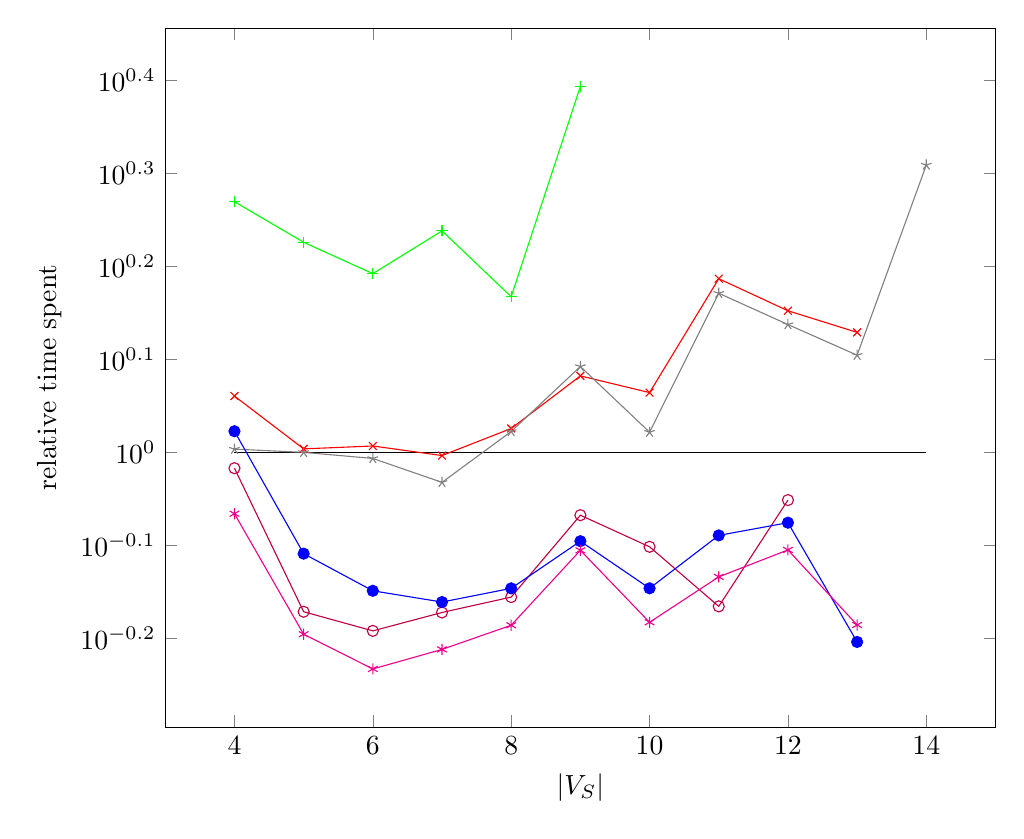
\begin{tikzpicture}
    \begin{axis}[
        xlabel=$|V_S|$,
        ylabel=relative time spent,
        ymode=log,
        legend style={at={(0.9,0.1)},anchor=south east},
        width=\textwidth,
		y tick label style={/pgf/number format/sci},
    ]
\addplot [mark=none, black] plot coordinates {
        (4,1) (14,1)};

   

\addplot[
        mark=x,
        red,
    ] plot coordinates {
        (4,1.149235278417448)
        (5,1.0083079007951214)
        (6,1.015552114217333)
        (7,0.9917637188145205)
        (8,1.060601873501574)
        (9,1.2080204277209134)
        (10,1.1590683500674202)
        (11,1.5368985401765969)
        (12,1.4196166165898805)
        (13,1.345479282144217)
};
%    \addlegendentry{DFS}


\addplot[
        mark=o,
        purple,
    ] plot coordinates {
        (4,0.9612291827097055)
        (5,0.6736846557006542)
        (6,0.6425091767491988)
        (7,0.6723934364944264)
        (8,0.6986220309175226)
        (9,0.8556489486454084)
        (10,0.7913299276289911)
        (11,0.6827413496042884)
        (12,0.8882442635255605)
};
%    \addlegendentry{GDFS O IP}


\addplot[
        mark=star,
        gray,
    ] plot coordinates {
        (4,1.0076438451392467)
        (5,0.9996588783961261)
        (6,0.9847179505164285)
        (7,0.9280395733234135)
        (8,1.052698920988995)
        (9,1.2364165435036165)
        (10,1.0508458659524293)
        (11,1.482398673483428)
        (12,1.3719047068368444)
        (13,1.2716510858517898)
        (14,2.0364819148591398)
};
%    \addlegendentry{GDFS C}


\addplot[
        mark=*,
        blue,
    ] plot coordinates {
        (4,1.0533520014717994)
        (5,0.7778922096030297)
        (6,0.7095420859821555)
        (7,0.690031519800899)
        (8,0.7138989512612041)
        (9,0.8022495198052423)
        (10,0.7139100327511367)
        (11,0.8138526765920138)
        (12,0.839844649957909)
        (13,0.6251267562387761)
};
%    \addlegendentry{K-Path}


\addplot[
        mark=+,
        green,
    ] plot coordinates {
        (4,1.8598817420849323)
        (5,1.6819321086529642)
        (6,1.5562633425290353)
        (7,1.7300402065586273)
        (8,1.4697328084299048)
        (9,2.4737693466393464)
};
%    \addlegendentry{CP}


\addplot[
        mark=asterisk,
        magenta,
    ] plot coordinates {
        (4,0.8587470004926293)
        (5,0.637211123426433)
        (6,0.5846797577876022)
        (7,0.6136474407419334)
        (8,0.6515146194296546)
        (9,0.7843995636829644)
        (10,0.6563231931888491)
        (11,0.7344868290598967)
        (12,0.7852380262879831)
        (13,0.6519427807384649)
};
%    \addlegendentry{GDFS A IP}


   

    \end{axis}
    \end{tikzpicture}


\caption{Serial}
\label{fig:sub1}
\end{subfigure}%
\begin{subfigure}{.5\linewidth}
\centering

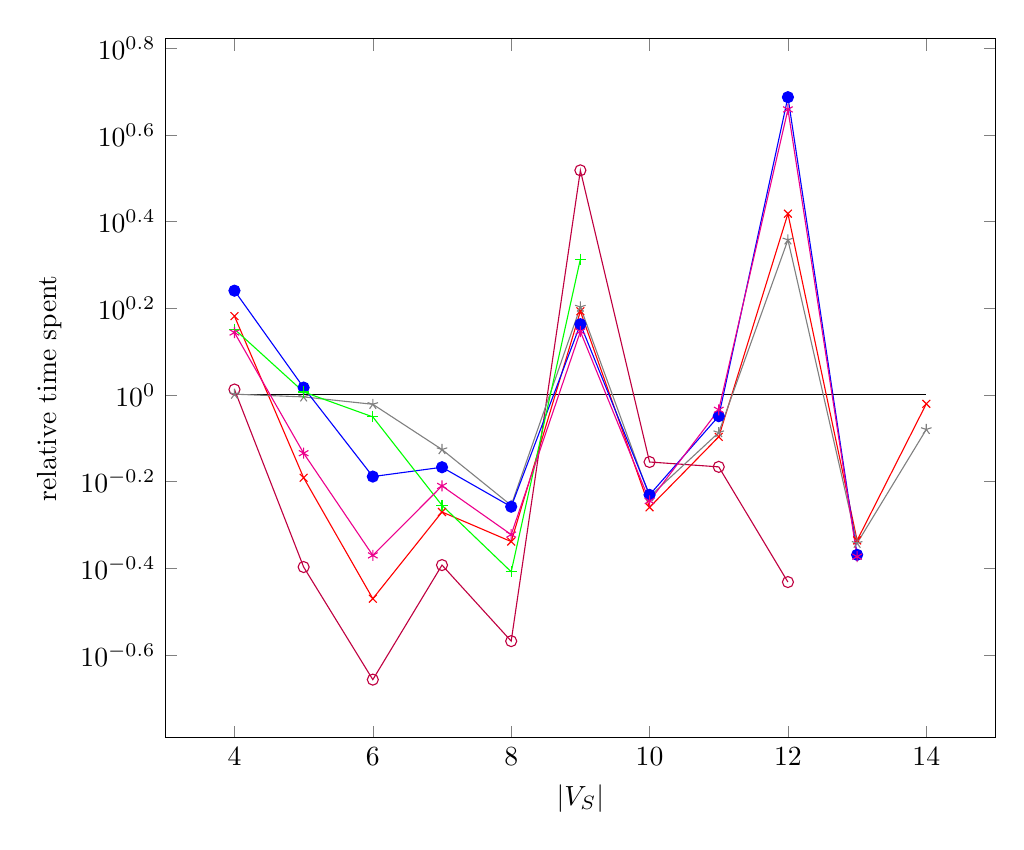
\begin{tikzpicture}
    \begin{axis}[
        xlabel=$|V_S|$,
        ylabel=relative time spent,
        ymode=log,
        legend style={at={(0.9,0.1)},anchor=south east},
        width=\textwidth,
		y tick label style={/pgf/number format/sci},
    ]
\addplot [mark=none, black] plot coordinates {
        (4,1) (14, 1)};




\addplot[
        mark=x,
        red,
    ] plot coordinates {
        (4,1.5196735481803552)
        (5,0.6439969153711)
        (6,0.3386925334619767)
        (7,0.5368610674342231)
        (8,0.45873474922274815)
        (9,1.5594868514866573)
        (10,0.5503271443080898)
        (11,0.8002158520089797)
        (12,2.618829716025611)
        (13,0.461660681606467)
        (14,0.9536983450489754)
};
%    \addlegendentry{DFS}


\addplot[
        mark=o,
        purple,
    ] plot coordinates {
        (4,1.0289639751297441)
        (5,0.40073099730691264)
        (6,0.2203309298278896)
        (7,0.40490458510733796)
        (8,0.2703553467095787)
        (9,3.2968841136523857)
        (10,0.7001969451830652)
        (11,0.6822506009880664)
        (12,0.37004898049509893)
};
%    \addlegendentry{GDFS O IP}


\addplot[
        mark=star,
        gray,
    ] plot coordinates {
        (4,1.0037860591934256)
        (5,0.9894012765779054)
        (6,0.9512995639254895)
        (7,0.7481500768569231)
        (8,0.5560328419142169)
        (9,1.5950594125932698)
        (10,0.5825880979420317)
        (11,0.8186254429321587)
        (12,2.2787645869722217)
        (13,0.4547207271773557)
        (14,0.8323681075075677)
};
%    \addlegendentry{GDFS C}


\addplot[
        mark=*,
        blue,
    ] plot coordinates {
        (4,1.739824792303458)
        (5,1.0396016144545588)
        (6,0.6479907091747379)
        (7,0.6809036260493723)
        (8,0.5520901104899674)
        (9,1.4556125513833869)
        (10,0.5879764504015326)
        (11,0.8930337054115022)
        (12,4.862531350090637)
        (13,0.4275493552859416)
};
%    \addlegendentry{K-Path}


\addplot[
        mark=+,
        green,
    ] plot coordinates {
        (4,1.4181640975707355)
        (5,1.0155919393670438)
        (6,0.8896407770170547)
        (7,0.5560547295333215)
        (8,0.3908257237814686)
        (9,2.0567874784311706)
};
%    \addlegendentry{CP}


\addplot[
        mark=asterisk,
        magenta,
    ] plot coordinates {
        (4,1.3928057135978327)
        (5,0.7336372164409364)
        (6,0.4262986752445699)
        (7,0.6165329994701355)
        (8,0.47610065673013646)
        (9,1.4003560173584488)
        (10,0.5691849125616277)
        (11,0.9238715681263124)
        (12,4.55583983031228)
        (13,0.4234248244588815)
};
%    \addlegendentry{GDFS A IP}
  

	
    \end{axis}
    \end{tikzpicture}

\caption{Cached}
\label{fig:sub2}
\end{subfigure}\\[1ex]
\begin{subfigure}{0.5\linewidth}
\centering

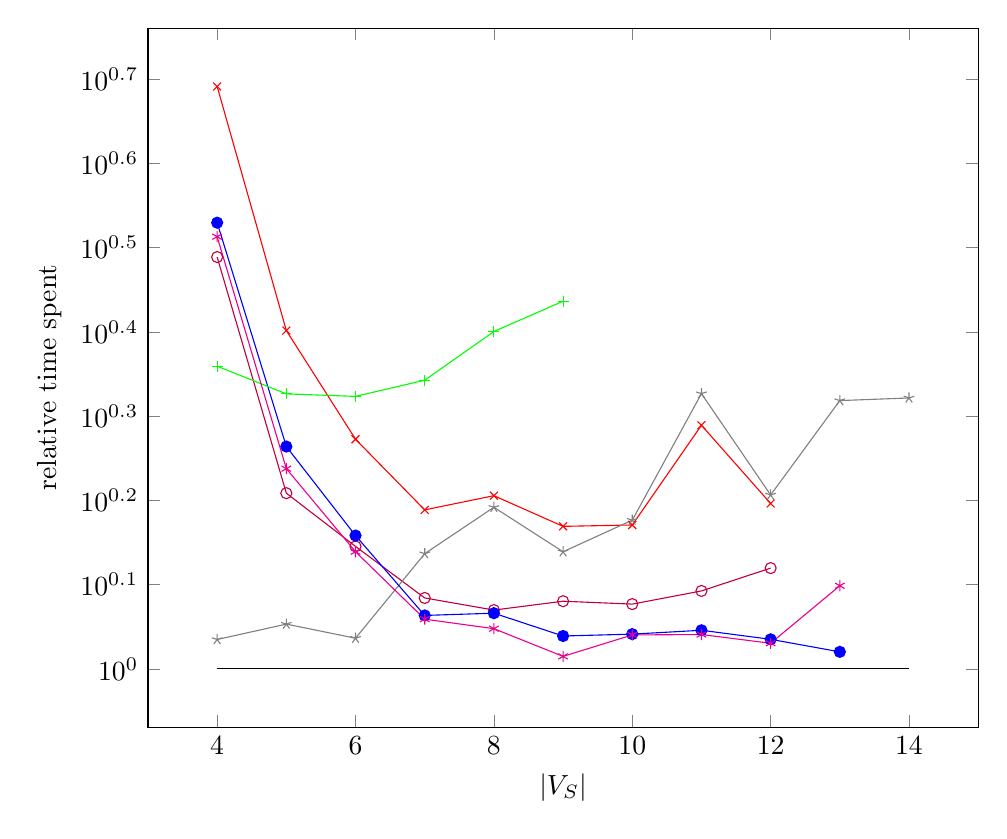
\begin{tikzpicture}
    \begin{axis}[
        xlabel=$|V_S|$,
        ylabel=relative time spent,
        ymode=log,
        legend style={at={(0.9,0.1)},anchor=south east},
        width=\textwidth,
		y tick label style={/pgf/number format/sci},
    ]
\addplot [mark=none, black] plot coordinates {
        (4,1) (14, 1)};


	

\addplot[
        mark=x,
        red,
    ] plot coordinates {
        (4,4.912635821328207)
        (5,2.5213322807291894)
        (6,1.8735281366916912)
        (7,1.5444862545247475)
        (8,1.6056787150146559)
        (9,1.4765521555469698)
        (10,1.4820555556240134)
        (11,1.946734238439349)
        (12,1.5718556269712267)
};
%    \addlegendentry{DFS}


\addplot[
        mark=o,
        purple,
    ] plot coordinates {
        (4,3.0822240524751128)
        (5,1.6165571205344698)
        (6,1.3978485397981901)
        (7,1.2140415216311997)
        (8,1.1745946191206549)
        (9,1.2032865829671746)
        (10,1.1937969470403793)
        (11,1.2375642924085462)
        (12,1.3172897955473268)
};
%    \addlegendentry{GDFS O IP}


\addplot[
        mark=star,
        gray,
    ] plot coordinates {
        (4,1.0837979979749324)
        (5,1.1303336976253304)
        (6,1.087572597425233)
        (7,1.3702576979065668)
        (8,1.5556435786427398)
        (9,1.3774635843717524)
        (10,1.5016451292498205)
        (11,2.122041244880633)
        (12,1.6087569895860554)
        (13,2.0820432556276365)
        (14,2.09712979447583)
};
%    \addlegendentry{GDFS C}


\addplot[
        mark=*,
        blue,
    ] plot coordinates {
        (4,3.38561160720786)
        (5,1.8365969772716313)
        (6,1.4398010790115316)
        (7,1.1574587494667208)
        (8,1.1645623226507533)
        (9,1.0941954726393444)
        (10,1.099782306968)
        (11,1.1114580211799494)
        (12,1.0842992282419759)
        (13,1.0478118522343631)
};
%    \addlegendentry{K-Path}


\addplot[
        mark=+,
        green,
    ] plot coordinates {
        (4,2.287168110582633)
        (5,2.120634315355006)
        (6,2.1061165486427873)
        (7,2.2013837152903006)
        (8,2.514842573582901)
        (9,2.731646143463003)
};
%    \addlegendentry{CP}


\addplot[
        mark=asterisk,
        magenta,
    ] plot coordinates {
        (4,3.2585173952994615)
        (5,1.728583400469593)
        (6,1.3775627829587174)
        (7,1.1456803324069784)
        (8,1.1162737735571762)
        (9,1.0349155153974534)
        (10,1.0973729419863378)
        (11,1.098601313310929)
        (12,1.0726988929900587)
        (13,1.2552103868339886)
};
%    \addlegendentry{GDFS A IP}

	
	
    \end{axis}
    \end{tikzpicture}

\caption{Parallel}
\label{fig:sub3}
\end{subfigure}
\begin{subfigure} {0.5\linewidth}
\centering

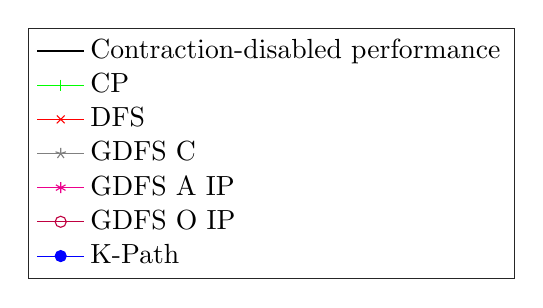
\begin{tikzpicture} 
    \begin{axis}[%
    hide axis,
    xmin=10,
    xmax=50,
    ymin=0,
    ymax=0.4,
    legend style={draw=white!15!black,legend cell align=left}
    ]
	\addlegendimage{black}
    \addlegendentry{Contraction-disabled performance}; 
     
    \addlegendimage{green, mark=+}
    \addlegendentry{CP};
    
    \addlegendimage{red, mark=x}
    \addlegendentry{DFS};
    
    \addlegendimage{gray, mark=star}
    \addlegendentry{GDFS C};
    
    \addlegendimage{magenta, mark=asterisk}
    \addlegendentry{GDFS A IP};
    
    \addlegendimage{purple, mark=o}
    \addlegendentry{GDFS O IP};
    
    \addlegendimage{blue, mark=*}
    \addlegendentry{K-Path};
    
    \end{axis}
\end{tikzpicture}

\end{subfigure}

\caption{Performance of our algorithm with \textbf{ZeroDomain} pruning using \textbf{`Labels and neighbours'} filtering relative to the performance of the algorithm without pruning. We avoid unnecessarily long paths, do not perform contraction and use the degree-based target graph vertex ordering. Data points above the black reference line denote that the pruning method introduces more delay, and data points below the reference line denote that the pruning method saves time. Note the logarithmic y-axis.}	
\label{fig:zerodomainlabelsneighbours}
\end{figure}


\begin{figure}
\begin{subfigure}{.5\linewidth}
\centering

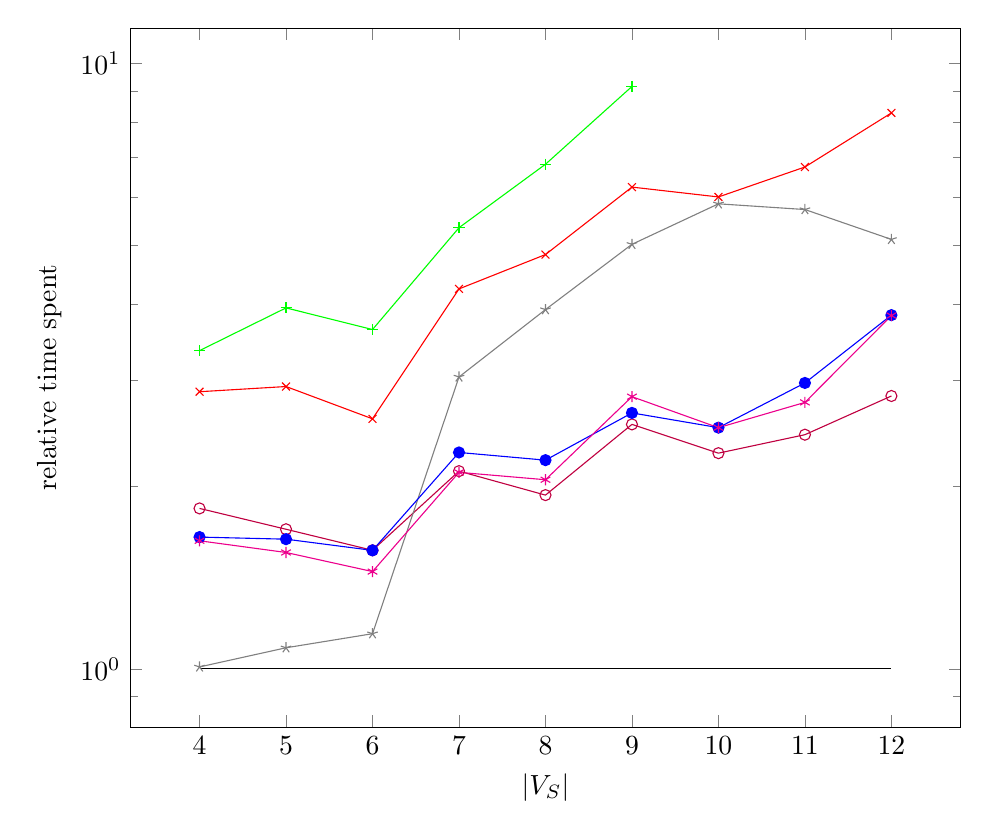
\begin{tikzpicture}
    \begin{axis}[
        xlabel=$|V_S|$,
        ylabel=relative time spent,
        ymode=log,
        legend style={at={(0.9,0.1)},anchor=south east},
        width=\textwidth,
		y tick label style={/pgf/number format/sci},
    ]
\addplot [mark=none, black] plot coordinates {
        (4,1) (12, 1)};

    

\addplot[
        mark=x,
        red,
    ] plot coordinates {
        (4,2.8681701535417203)
        (5,2.9254018783511473)
        (6,2.5872798141640203)
        (7,4.239345235159544)
        (8,4.830571894920121)
        (9,6.242761798378523)
        (10,6.013058042923716)
        (11,6.738597774875578)
        (12,8.275599621231075)
};
%    \addlegendentry{DFS}


\addplot[
        mark=o,
        purple,
    ] plot coordinates {
        (4,1.8408080356188123)
        (5,1.7005582324670065)
        (6,1.56989493549955)
        (7,2.1207796500463942)
        (8,1.9363735218126932)
        (9,2.533248243975908)
        (10,2.2707880019469786)
        (11,2.4359352917004715)
        (12,2.821912275157622)
};
%    \addlegendentry{GDFS O IP}


\addplot[
        mark=star,
        gray,
    ] plot coordinates {
        (4,1.0076654131165232)
        (5,1.0837612058063686)
        (6,1.1432927339149115)
        (7,3.033634347762899)
        (8,3.919309944661518)
        (9,5.022580039736159)
        (10,5.858260568094502)
        (11,5.732626441781628)
        (12,5.117036438110539)
};
%    \addlegendentry{GDFS C}


\addplot[
        mark=*,
        blue,
    ] plot coordinates {
        (4,1.6507129093587034)
        (5,1.6376785905633322)
        (6,1.5694034681484315)
        (7,2.2768378662823556)
        (8,2.2111751094243637)
        (9,2.6460554936280003)
        (10,2.5019612966868143)
        (11,2.9653929534687484)
        (12,3.8377325981845987)
};
%    \addlegendentry{K-Path}


\addplot[
        mark=+,
        green,
    ] plot coordinates {
        (4,3.3530620508044278)
        (5,3.945082943073584)
        (6,3.633181121338477)
        (7,5.349792316707754)
        (8,6.809444287637352)
        (9,9.151106021332374)
};
%    \addlegendentry{CP}


\addplot[
        mark=asterisk,
        magenta,
    ] plot coordinates {
        (4,1.6276085621719778)
        (5,1.5567783428027056)
        (6,1.447868814386046)
        (7,2.111238924804706)
        (8,2.052589583126582)
        (9,2.8147150464658517)
        (10,2.5017899929941634)
        (11,2.7540625611814193)
        (12,3.831399427105856)
};
%    \addlegendentry{GDFS A IP}

   

    \end{axis}
    \end{tikzpicture}


\caption{serial}
\label{fig:sub1}
\end{subfigure}%
\begin{subfigure}{.5\linewidth}
\centering

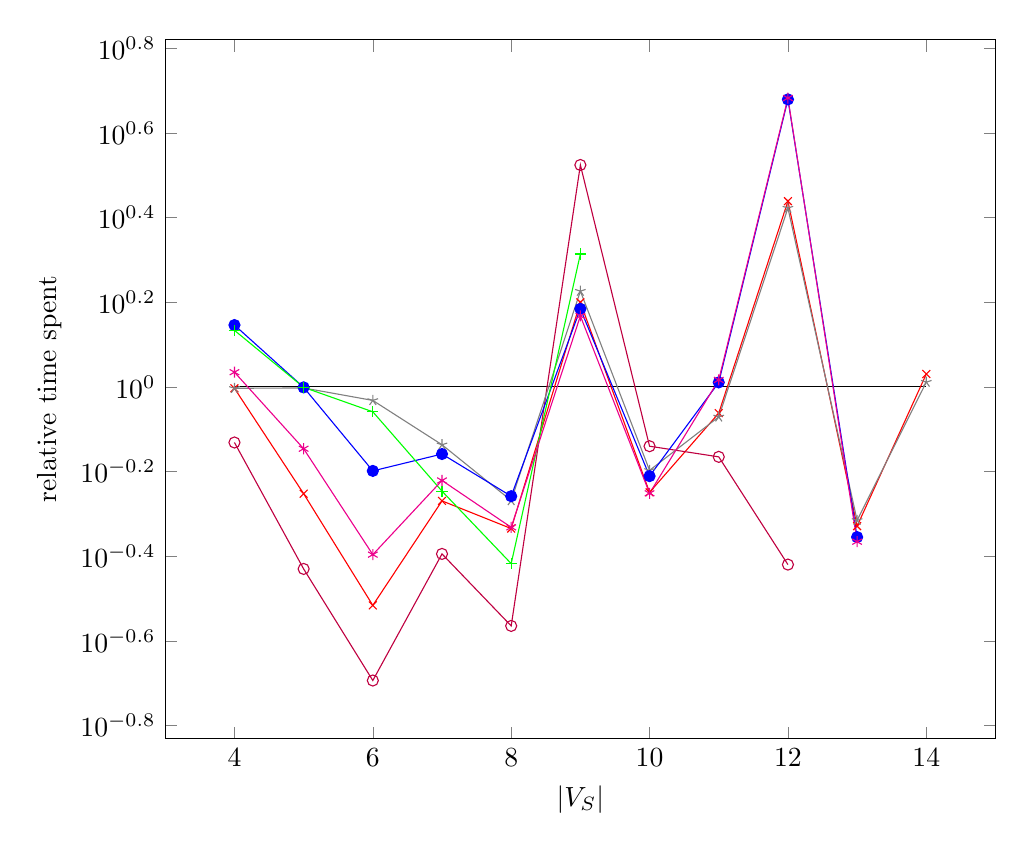
\begin{tikzpicture}
    \begin{axis}[
        xlabel=$|V_S|$,
        ylabel=relative time spent,
        ymode=log,
        legend style={at={(0.9,0.1)},anchor=south east},
        width=\textwidth,
		y tick label style={/pgf/number format/sci},
    ]
\addplot [mark=none, black] plot coordinates {
        (4,1) (14, 1)};


	

\addplot[
        mark=x,
        red,
    ] plot coordinates {
        (4,0.9923899104921649)
        (5,0.5595066683253078)
        (6,0.3048945865180337)
        (7,0.5381004704636452)
        (8,0.4628899334014771)
        (9,1.5833880688615796)
        (10,0.563696852962109)
        (11,0.8669963898068426)
        (12,2.745349524198522)
        (13,0.4690924414042419)
        (14,1.0728242665153411)
};
%    \addlegendentry{DFS}


\addplot[
        mark=o,
        purple,
    ] plot coordinates {
        (4,0.739244200124882)
        (5,0.3717240182715724)
        (6,0.20260979424571846)
        (7,0.40328082248328134)
        (8,0.2726428806815875)
        (9,3.342614987755728)
        (10,0.7244476709108397)
        (11,0.6836929828863543)
        (12,0.3805696273086222)
};
%    \addlegendentry{GDFS O IP}


\addplot[
        mark=star,
        gray,
    ] plot coordinates {
        (4,0.9924896603950555)
        (5,0.994360434712658)
        (6,0.9291538705872268)
        (7,0.730196682594658)
        (8,0.5390873818404287)
        (9,1.6832008614785352)
        (10,0.6352356062289578)
        (11,0.8496501176486361)
        (12,2.6445551844487807)
        (13,0.4840033554409139)
        (14,1.026259804661441)
};
%    \addlegendentry{GDFS C}


\addplot[
        mark=*,
        blue,
    ] plot coordinates {
        (4,1.3997982449312394)
        (5,0.997525391259792)
        (6,0.6333756640426693)
        (7,0.6943303320196079)
        (8,0.5519684346380963)
        (9,1.5286729452268917)
        (10,0.6156583962202479)
        (11,1.024740262929912)
        (12,4.774734990588401)
        (13,0.4419374709287728)
};
%    \addlegendentry{K-Path}


\addplot[
        mark=+,
        green,
    ] plot coordinates {
        (4,1.3603876642406472)
        (5,0.9977315311707801)
        (6,0.8734385188908586)
        (7,0.5673919611448295)
        (8,0.3826349700684204)
        (9,2.0597652911938544)
};
%    \addlegendentry{CP}


\addplot[
        mark=asterisk,
        magenta,
    ] plot coordinates {
        (4,1.0832036968767507)
        (5,0.714551103294575)
        (6,0.4017364306204272)
        (7,0.6012055707935953)
        (8,0.4660022392983759)
        (9,1.4709429657453295)
        (10,0.5607915060867077)
        (11,1.0386348465457822)
        (12,4.8097603627365055)
        (13,0.43097398458603053)
};
%    \addlegendentry{GDFS A IP}

	
    \end{axis}
    \end{tikzpicture}

\caption{cached}
\label{fig:sub2}
\end{subfigure}\\[1ex]
\begin{subfigure}{0.5\linewidth}
\centering

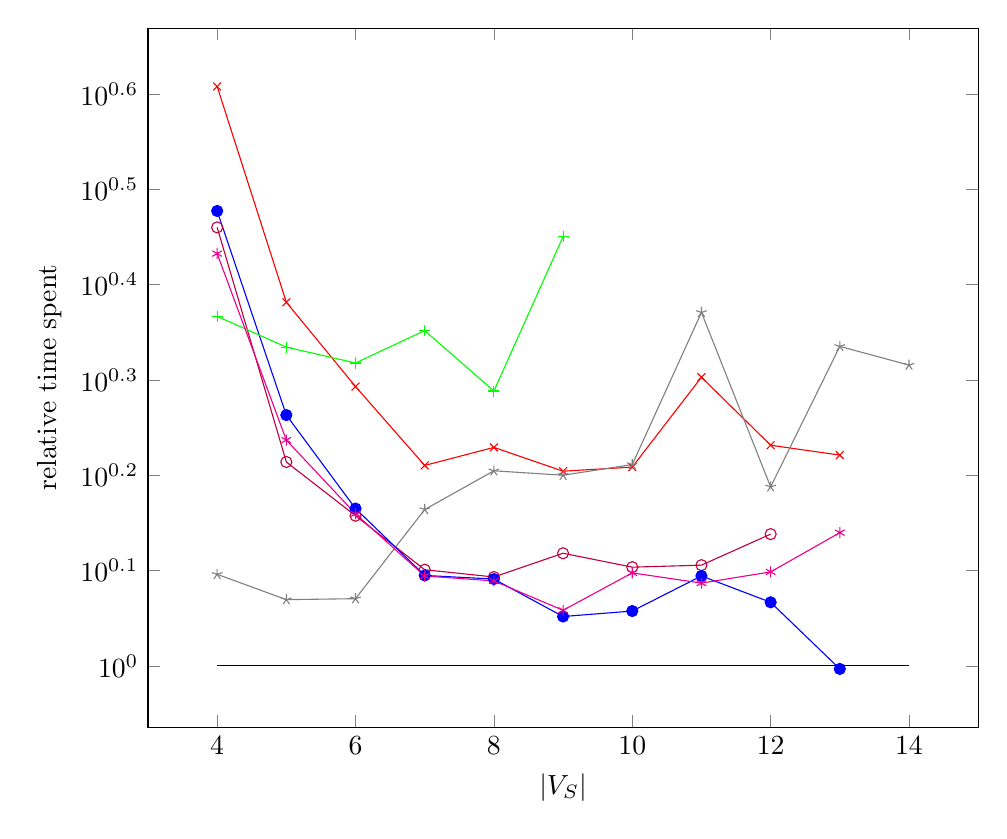
\begin{tikzpicture}
    \begin{axis}[
        xlabel=$|V_S|$,
        ylabel=relative time spent,
        ymode=log,
        legend style={at={(0.9,0.1)},anchor=south east},
        width=\textwidth,
		y tick label style={/pgf/number format/sci},
    ]
\addplot [mark=none, black] plot coordinates {
        (4,1) (14, 1)};



\addplot[
        mark=x,
        red,
    ] plot coordinates {
        (4,4.055665332528571)
        (5,2.4079068291217)
        (6,1.9643320384841314)
        (7,1.6232718485965263)
        (8,1.6955903014633646)
        (9,1.6008062270872792)
        (10,1.6167961960677952)
        (11,2.008933357310069)
        (12,1.704410962543426)
        (13,1.6643657926641058)
};
%    \addlegendentry{DFS}


\addplot[
        mark=o,
        purple,
    ] plot coordinates {
        (4,2.8851878090262195)
        (5,1.636942509871993)
        (6,1.4374997042728976)
        (7,1.2616655204621405)
        (8,1.2396952026488233)
        (9,1.3129460412244731)
        (10,1.269489134852407)
        (11,1.2756554118663406)
        (12,1.3750472085101815)
};
%    \addlegendentry{GDFS O IP}


\addplot[
        mark=star,
        gray,
    ] plot coordinates {
        (4,1.2478328793750295)
        (5,1.1736817816635776)
        (6,1.1764101574372858)
        (7,1.4592075490444798)
        (8,1.6024676243054734)
        (9,1.5853180312626138)
        (10,1.6267475153944102)
        (11,2.3492273224066422)
        (12,1.541367629203128)
        (13,2.1643253277100984)
        (14,2.068648556937112)
};
%    \addlegendentry{GDFS C}


\addplot[
        mark=*,
        blue,
    ] plot coordinates {
        (4,3.002052014953125)
        (5,1.8333632864658882)
        (6,1.4625868876088735)
        (7,1.244428892395309)
        (8,1.2334917943953325)
        (9,1.1267969028185083)
        (10,1.1417960691621196)
        (11,1.242845045792521)
        (12,1.1662050312002787)
        (13,0.9927656897482176)
};
%    \addlegendentry{K-Path}


\addplot[
        mark=+,
        green,
    ] plot coordinates {
        (4,2.327075300876756)
        (5,2.160407689989366)
        (6,2.0792574180238432)
        (7,2.248434541176637)
        (8,1.943200046149185)
        (9,2.82171519727411)
};
%    \addlegendentry{CP}


\addplot[
        mark=asterisk,
        magenta,
    ] plot coordinates {
        (4,2.7083657638964724)
        (5,1.7258042096013082)
        (6,1.4441565938470444)
        (7,1.2427090481371263)
        (8,1.2279821585739619)
        (9,1.1438554945469597)
        (10,1.252073988123748)
        (11,1.2215012813271526)
        (12,1.2550832966834882)
        (13,1.3798442157135253)
};
%    \addlegendentry{GDFS A IP}

	
    \end{axis}
    \end{tikzpicture}

\caption{parallel}
\label{fig:sub3}
\end{subfigure}
\begin{subfigure} {0.5\linewidth}
\centering

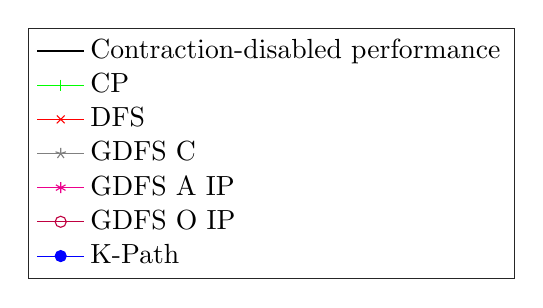
\begin{tikzpicture} 
    \begin{axis}[%
    hide axis,
    xmin=10,
    xmax=50,
    ymin=0,
    ymax=0.4,
    legend style={draw=white!15!black,legend cell align=left}
    ]
	\addlegendimage{black}
    \addlegendentry{Contraction-disabled performance}; 
     
    \addlegendimage{green, mark=+}
    \addlegendentry{CP};
    
    \addlegendimage{red, mark=x}
    \addlegendentry{DFS};
    
    \addlegendimage{gray, mark=star}
    \addlegendentry{GDFS C};
    
    \addlegendimage{magenta, mark=asterisk}
    \addlegendentry{GDFS A IP};
    
    \addlegendimage{purple, mark=o}
    \addlegendentry{GDFS O IP};
    
    \addlegendimage{blue, mark=*}
    \addlegendentry{K-Path};
    
    \end{axis}
\end{tikzpicture}

\end{subfigure}

\caption{Performance of our algorithm with \textbf{ZeroDomain} pruning using \textbf{`Free neighbours'} filtering relative to the performance of the algorithm without pruning. We avoid unnecessarily long paths, do not perform contraction and use the degree-based target graph vertex ordering. Data points above the black reference line denote that the pruning method introduces more delay, and data points below the reference line denote that the pruning method saves time. Note the logarithmic y-axis.}	
\label{fig:zerodomainunmatched}
\end{figure}

\begin{figure}
\begin{subfigure}{.5\linewidth}
\centering

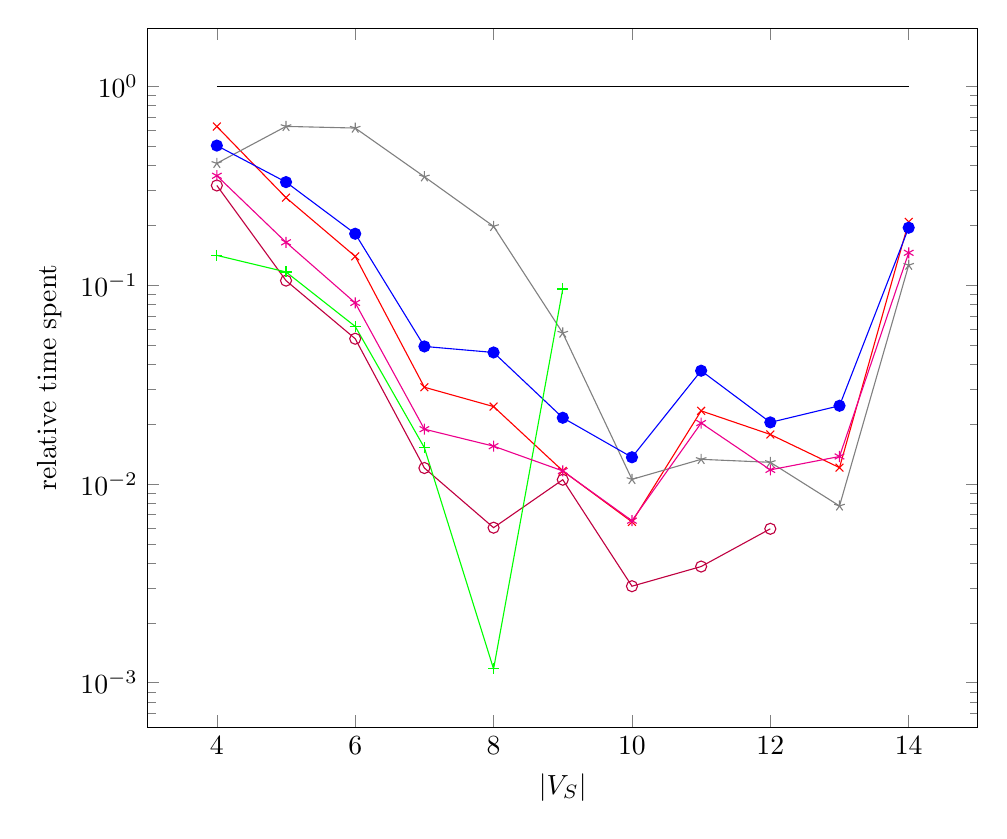
\begin{tikzpicture}
        \begin{axis}[
        xlabel=$|V_S|$,
        ylabel=relative time spent,
        ymode=log,
        legend style={at={(0.9,0.1)},anchor=south east},
        width=\textwidth,
		y tick label style={/pgf/number format/sci},
    ]
\addplot [mark=none, black] plot coordinates {
        (4,1) (14, 1)};



\addplot[
        mark=x,
        red,
    ] plot coordinates {
        (4,0.6287543277612293)
        (5,0.2757977099154991)
        (6,0.1396777930920231)
        (7,0.030673609879429353)
        (8,0.02451224889378789)
        (9,0.011639988009323088)
        (10,0.006444926208946211)
        (11,0.023332165971646113)
        (12,0.017747881691377088)
        (13,0.012081584812504542)
        (14,0.20827170338997036)
};
%    \addlegendentry{DFS}


\addplot[
        mark=o,
        purple,
    ] plot coordinates {
        (4,0.31762184661225146)
        (5,0.10548661997054809)
        (6,0.05380597268481946)
        (7,0.012031104647835078)
        (8,0.006026685633755746)
        (9,0.010506576117209399)
        (10,0.003059622842895182)
        (11,0.0038425576274282447)
        (12,0.005950005569221872)
};
%    \addlegendentry{GDFS O IP}


\addplot[
        mark=star,
        gray,
    ] plot coordinates {
        (4,0.4106300255336265)
        (5,0.6297150335729914)
        (6,0.6177849466375939)
        (7,0.3514224232413242)
        (8,0.1978056188420405)
        (9,0.05747899493182684)
        (10,0.01054844071183747)
        (11,0.013304423784248232)
        (12,0.01285276131493418)
        (13,0.007754862312966293)
        (14,0.12620402164239297)
};
%    \addlegendentry{GDFS C}


\addplot[
        mark=*,
        blue,
    ] plot coordinates {
        (4,0.5042771733798161)
        (5,0.33026481004490515)
        (6,0.1815749814615767)
        (7,0.04920860049799136)
        (8,0.04588175630434421)
        (9,0.02153377003082302)
        (10,0.013622516633218007)
        (11,0.037145391651794424)
        (12,0.02041196505471854)
        (13,0.024748365975288622)
        (14,0.19477391590054371)
};
%    \addlegendentry{K-Path}


\addplot[
        mark=+,
        green,
    ] plot coordinates {
        (4,0.14129388384266495)
        (5,0.11661297643581336)
        (6,0.062037664925466474)
        (7,0.015214384516616386)
        (8,0.001173447995948207)
        (9,0.09577023175742294)
};
%    \addlegendentry{CP}


\addplot[
        mark=asterisk,
        magenta,
    ] plot coordinates {
        (4,0.35547913440959544)
        (5,0.16441492185647066)
        (6,0.081522356518962)
        (7,0.01887115321256927)
        (8,0.015496754850373495)
        (9,0.01163137758041799)
        (10,0.0065360121014294)
        (11,0.02025243713993974)
        (12,0.011777226097555493)
        (13,0.013750262714309236)
        (14,0.1456191628467376)
};
%    \addlegendentry{GDFS A IP}


   

    \end{axis}
    \end{tikzpicture}


\caption{serial}
\label{fig:sub1}
\end{subfigure}%
\begin{subfigure}{.5\linewidth}
\centering

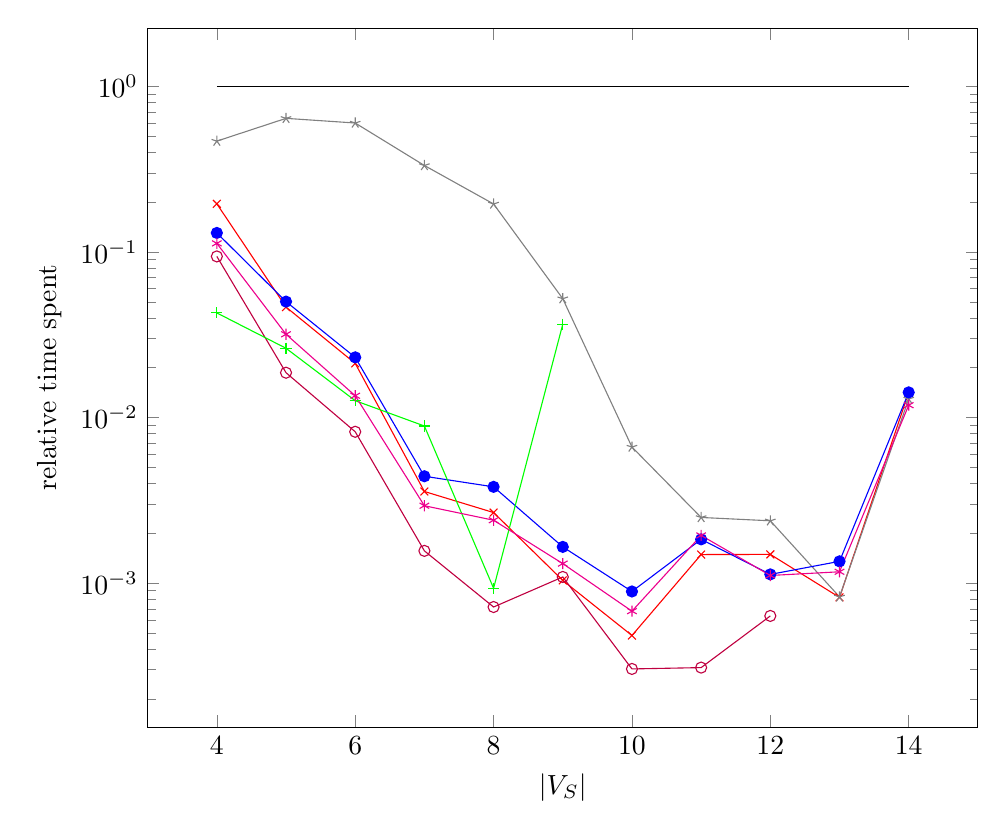
\begin{tikzpicture}
       \begin{axis}[
        xlabel=$|V_S|$,
        ylabel=relative time spent,
        ymode=log,
        legend style={at={(0.9,0.1)},anchor=south east},
        width=\textwidth,
		y tick label style={/pgf/number format/sci},
    ]
\addplot [mark=none, black] plot coordinates {
        (4,1) (14, 1)};



\addplot[
        mark=x,
        red,
    ] plot coordinates {
        (4,0.19553736011435197)
        (5,0.04651353813878456)
        (6,0.021254007864093483)
        (7,0.003578003137043706)
        (8,0.002669239461236206)
        (9,0.001038638013086457)
        (10,4.827831034437402E-4)
        (11,0.0014882311568104045)
        (12,0.0014918153191871841)
        (13,8.201888846909311E-4)
        (14,0.014177555092282024)
};
%    \addlegendentry{DFS}


\addplot[
        mark=o,
        purple,
    ] plot coordinates {
        (4,0.0940851187730316)
        (5,0.018669179394963042)
        (6,0.008210777047784168)
        (7,0.00156671351986859)
        (8,7.175769161658074E-4)
        (9,0.0010901108792181757)
        (10,3.032823855272371E-4)
        (11,3.089718288207255E-4)
        (12,6.339461008270098E-4)
};
%    \addlegendentry{GDFS O IP}


\addplot[
        mark=star,
        gray,
    ] plot coordinates {
        (4,0.46776174984809504)
        (5,0.6418994975058616)
        (6,0.6016705469416976)
        (7,0.33331288068306)
        (8,0.19516359829459384)
        (9,0.052258028899510256)
        (10,0.00663966390973203)
        (11,0.002493325643069144)
        (12,0.002380331383759815)
        (13,8.261279519951037E-4)
        (14,0.012952744336981126)
};
%    \addlegendentry{GDFS C}


\addplot[
        mark=*,
        blue,
    ] plot coordinates {
        (4,0.13042500432875637)
        (5,0.050180114187121205)
        (6,0.023114568588865403)
        (7,0.004422648284462927)
        (8,0.0038176084846363034)
        (9,0.0016559892479824923)
        (10,8.905816418131041E-4)
        (11,0.0018391391340257801)
        (12,0.0011295780527541543)
        (13,0.0013542664491973389)
        (14,0.01420206790590417)
};
%    \addlegendentry{K-Path}


\addplot[
        mark=+,
        green,
    ] plot coordinates {
        (4,0.0428754303586345)
        (5,0.026223845245723965)
        (6,0.012652891562625723)
        (7,0.008896499518256218)
        (8,9.31591774671725E-4)
        (9,0.03666836072401081)
};
%    \addlegendentry{CP}


\addplot[
        mark=asterisk,
        magenta,
    ] plot coordinates {
        (4,0.11278665322864612)
        (5,0.03186942103424617)
        (6,0.013551849864991583)
        (7,0.0029347571062988687)
        (8,0.0023993757390741166)
        (9,0.001312317141160979)
        (10,6.774056453796584E-4)
        (11,0.0019421604989434682)
        (12,0.0011128003583009694)
        (13,0.0011711624655019737)
        (14,0.011878755635911897)
};
%    \addlegendentry{GDFS A IP}

	
	
    \end{axis}
    \end{tikzpicture}

\caption{cached}
\label{fig:sub2}
\end{subfigure}\\[1ex]
\begin{subfigure}{0.5\linewidth}
\centering

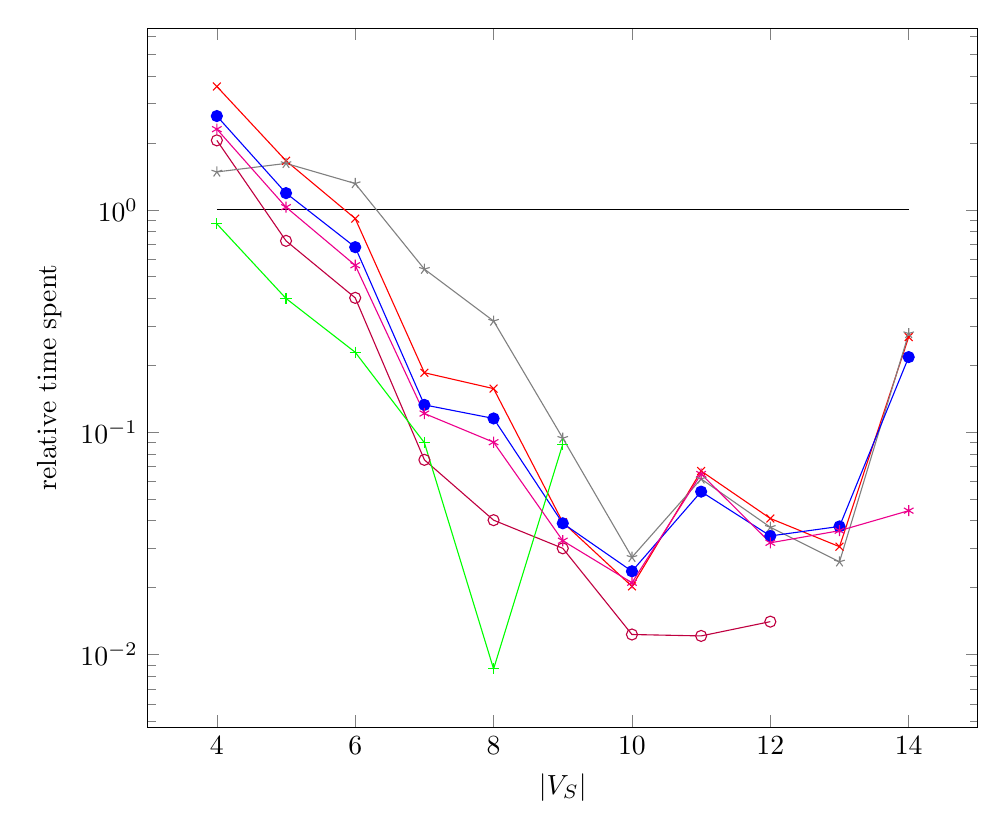
\begin{tikzpicture}
    \begin{axis}[
        xlabel=$|V_S|$,
        ylabel=relative time spent,
        ymode=log,
        legend style={at={(0.9,0.1)},anchor=south east},
        width=\textwidth,
		y tick label style={/pgf/number format/sci},
    ]
\addplot [mark=none, black] plot coordinates {
        (4,1) (14, 1)};



\addplot[
        mark=x,
        red,
    ] plot coordinates {
        (4,3.5863917566717767)
        (5,1.6614170135257829)
        (6,0.913341561725058)
        (7,0.18513401953197028)
        (8,0.15706371851369083)
        (9,0.039380360092514)
        (10,0.020272354245869484)
        (11,0.06693875268275729)
        (12,0.04094655208604481)
        (13,0.03057385975605409)
        (14,0.26792292492149405)
};
%    \addlegendentry{DFS}


\addplot[
        mark=o,
        purple,
    ] plot coordinates {
        (4,2.052763630992859)
        (5,0.7252220094219901)
        (6,0.4019908919869054)
        (7,0.0751392967924247)
        (8,0.0402321588998491)
        (9,0.030063816263190213)
        (10,0.012316567212513396)
        (11,0.012136049821184658)
        (12,0.01407028044173897)
};
%    \addlegendentry{GDFS O IP}


\addplot[
        mark=star,
        gray,
    ] plot coordinates {
        (4,1.4803263312981985)
        (5,1.617088480231661)
        (6,1.312985590310922)
        (7,0.541000232064156)
        (8,0.31621413493384876)
        (9,0.09404453831749748)
        (10,0.027408496020476347)
        (11,0.061673144974397576)
        (12,0.03739780619521971)
        (13,0.02614141264184211)
        (14,0.2777072903785752)
};
%    \addlegendentry{GDFS C}


\addplot[
        mark=*,
        blue,
    ] plot coordinates {
        (4,2.640444380229205)
        (5,1.1886881061231498)
        (6,0.6793824205820389)
        (7,0.13271318550783862)
        (8,0.11533183769943123)
        (9,0.038955674057646106)
        (10,0.023698433402264296)
        (11,0.0540615523126724)
        (12,0.034171466937311545)
        (13,0.03771279726019261)
        (14,0.21769075053049192)
};
%    \addlegendentry{K-Path}


\addplot[
        mark=+,
        green,
    ] plot coordinates {
        (4,0.8650360306803884)
        (5,0.39951182944872243)
        (6,0.2288811300337159)
        (7,0.0896782754536235)
        (8,0.008624199068128502)
        (9,0.08847130248188806)
};
%    \addlegendentry{CP}


\addplot[
        mark=asterisk,
        magenta,
    ] plot coordinates {
        (4,2.3056130434020963)
        (5,1.0279513694895468)
        (6,0.5632528558219363)
        (7,0.12138481892093078)
        (8,0.09017283243188468)
        (9,0.03252156535486139)
        (10,0.02104885765787201)
        (11,0.06488806314689854)
        (12,0.031829464045399214)
        (13,0.03607848508196143)
        (14,0.04438987254212279)
};
%    \addlegendentry{GDFS A IP}

	
    \end{axis}
    \end{tikzpicture}

\caption{parallel}
\label{fig:sub3}
\end{subfigure}
\begin{subfigure} {0.5\linewidth}
\centering

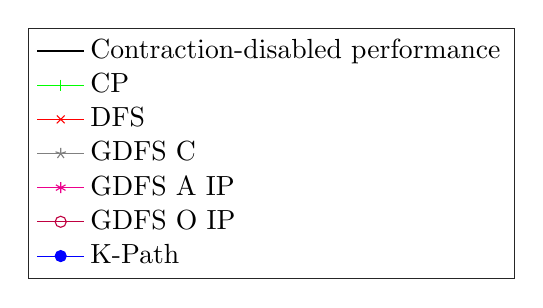
\begin{tikzpicture} 
    \begin{axis}[%
    hide axis,
    xmin=10,
    xmax=50,
    ymin=0,
    ymax=0.4,
    legend style={draw=white!15!black,legend cell align=left}
    ]
	\addlegendimage{black}
    \addlegendentry{Contraction-disabled performance}; 
     
    \addlegendimage{green, mark=+}
    \addlegendentry{CP};
    
    \addlegendimage{red, mark=x}
    \addlegendentry{DFS};
    
    \addlegendimage{gray, mark=star}
    \addlegendentry{GDFS C};
    
    \addlegendimage{magenta, mark=asterisk}
    \addlegendentry{GDFS A IP};
    
    \addlegendimage{purple, mark=o}
    \addlegendentry{GDFS O IP};
    
    \addlegendimage{blue, mark=*}
    \addlegendentry{K-Path};
    
    \end{axis}
\end{tikzpicture}

\end{subfigure}

\caption{Performance of our algorithm with \textbf{ZeroDomain} pruning using \textbf{`M-filtering'} filtering relative to the performance of the algorithm without pruning. We avoid unnecessarily long paths, do not perform contraction and use the degree-based target graph vertex ordering. Data points above the black reference line denote that the pruning method introduces more delay, and data points below the reference line denote that the pruning method saves time. Note the logarithmic y-axis.}	
\label{fig:zerodomainmfiltering}
\end{figure}

\begin{figure}
\begin{subfigure}{.5\linewidth}
\centering

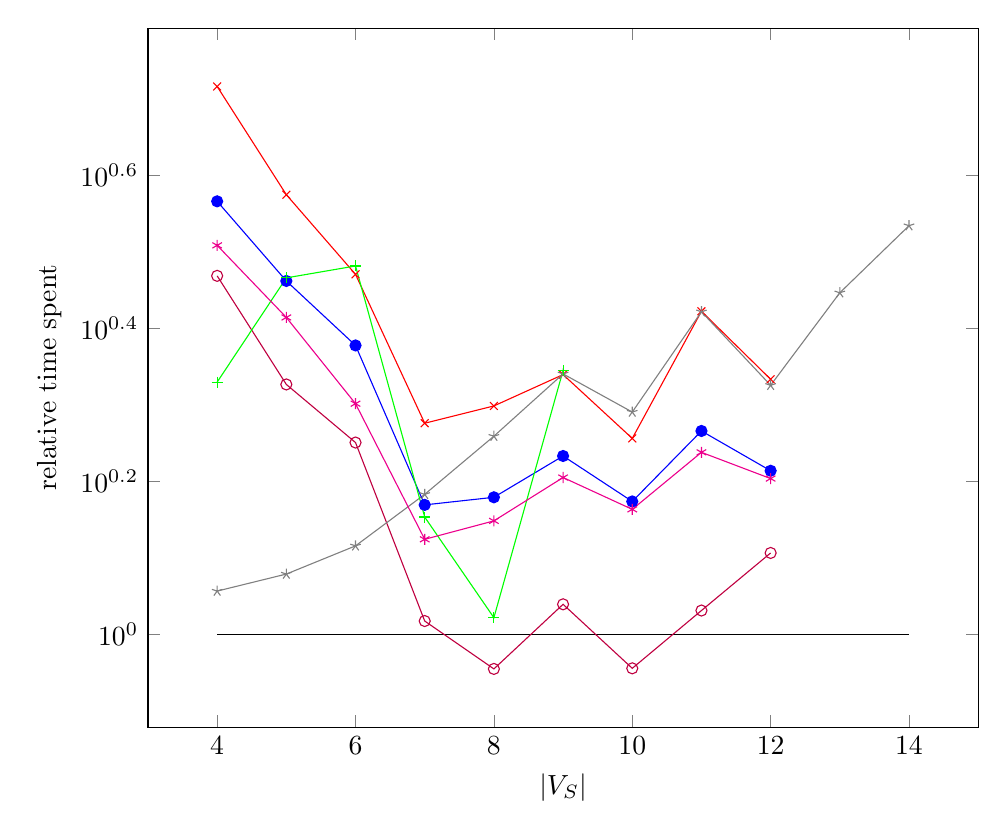
\begin{tikzpicture}
        \begin{axis}[
        xlabel=$|V_S|$,
        ylabel=relative time spent,
        ymode=log,
        legend style={at={(0.9,0.1)},anchor=south east},
        width=\textwidth,
		y tick label style={/pgf/number format/sci},
    ]
\addplot [mark=none, black] plot coordinates {
        (4,1) (14, 1)};

    
   

\addplot[
        mark=x,
        red,
    ] plot coordinates {
        (4,5.202946551261944)
        (5,3.756162046192574)
        (6,2.9549254023879072)
        (7,1.8872742557474473)
        (8,1.9880582223277101)
        (9,2.1847812854733193)
        (10,1.8028559351037163)
        (11,2.6436531391416507)
        (12,2.1539273359082483)
};
%    \addlegendentry{DFS}


\addplot[
        mark=o,
        purple,
    ] plot coordinates {
        (4,2.9414858115997387)
        (5,2.120863031356877)
        (6,1.7804930224229873)
        (7,1.0400701807728874)
        (8,0.9003554054490217)
        (9,1.0937936596519373)
        (10,0.9019831415298204)
        (11,1.0734764108654673)
        (12,1.2767276824510232)
};
%    \addlegendentry{GDFS O IP}


\addplot[
        mark=star,
        gray,
    ] plot coordinates {
        (4,1.1382355278673217)
        (5,1.198063456290179)
        (6,1.3042425098741526)
        (7,1.5233183009320665)
        (8,1.8148828000886499)
        (9,2.189451318312936)
        (10,1.9518249758925157)
        (11,2.639768817120566)
        (12,2.1154918845964863)
        (13,2.7952098947822313)
        (14,3.4210781907374623)
};
%    \addlegendentry{GDFS C}


\addplot[
        mark=*,
        blue,
    ] plot coordinates {
        (4,3.6819210072894446)
        (5,2.896400619358773)
        (6,2.3852188316658136)
        (7,1.4756755823523737)
        (8,1.5098085945063882)
        (9,1.7097753943529064)
        (10,1.490937989140139)
        (11,1.8438583447137513)
        (12,1.635315159939935)
};
%    \addlegendentry{K-Path}


\addplot[
        mark=+,
        green,
    ] plot coordinates {
        (4,2.1359021980392736)
        (5,2.923428609692478)
        (6,3.0304568963312812)
        (7,1.4225695726266137)
        (8,1.0506565420981449)
        (9,2.212314905046649)
};
%    \addlegendentry{CP}


\addplot[
        mark=asterisk,
        magenta,
    ] plot coordinates {
        (4,3.2242822734185275)
        (5,2.5950345747500103)
        (6,2.0014242504647624)
        (7,1.3303134982815363)
        (8,1.4062726411755775)
        (9,1.6024494454371436)
        (10,1.4559250035524376)
        (11,1.7288683972843149)
        (12,1.5973164420401704)
};
%    \addlegendentry{GDFS A IP}


    \end{axis}
    \end{tikzpicture}


\caption{serial}
\label{fig:sub1}
\end{subfigure}%
\begin{subfigure}{.5\linewidth}
\centering

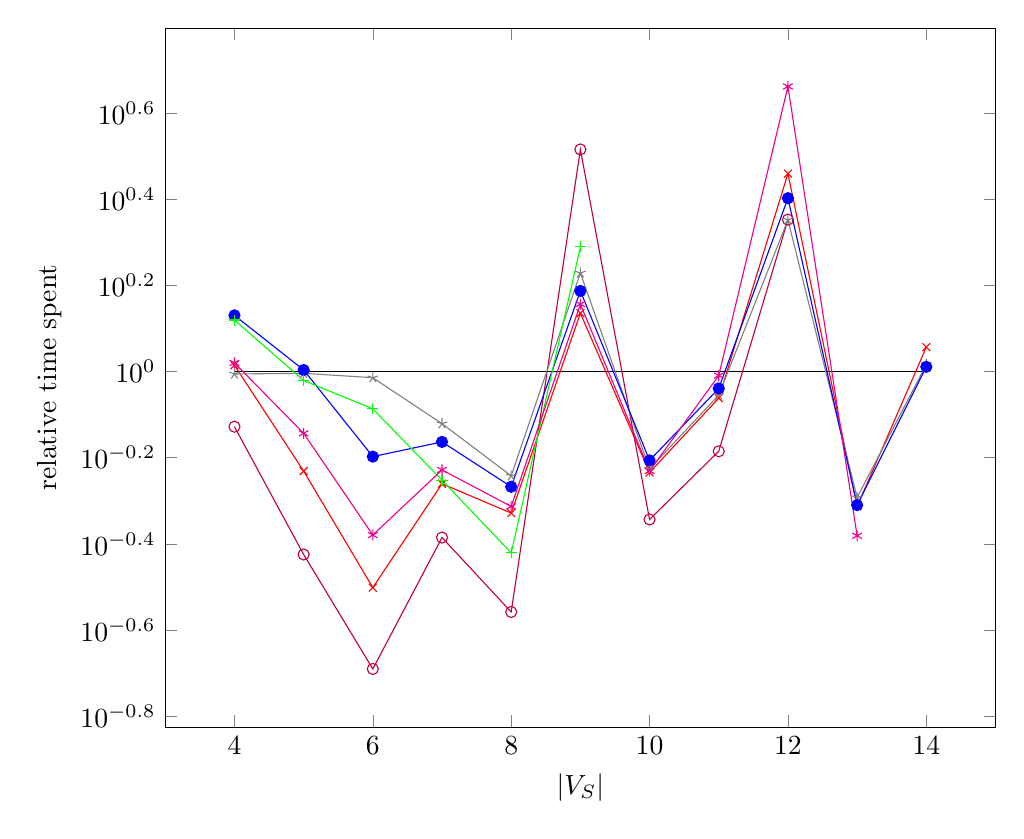
\begin{tikzpicture}
    \begin{axis}[
        xlabel=$|V_S|$,
        ylabel=relative time spent,
        ymode=log,
        legend style={at={(0.9,0.1)},anchor=south east},
        width=\textwidth,
		y tick label style={/pgf/number format/sci},
    ]
\addplot [mark=none, black] plot coordinates {
        (4,1) (14, 1)};



\addplot[
        mark=x,
        red,
    ] plot coordinates {
        (4,1.0341963936340537)
        (5,0.5872212498317262)
        (6,0.3150252343592421)
        (7,0.5489328540502025)
        (8,0.4691563660507788)
        (9,1.3659267214920254)
        (10,0.5829158055427053)
        (11,0.8675410228213514)
        (12,2.8804215346851567)
        (13,0.48622042850802205)
        (14,1.139249103225921)
};
%    \addlegendentry{DFS}


\addplot[
        mark=o,
        purple,
    ] plot coordinates {
        (4,0.7446160731342548)
        (5,0.3760872484757529)
        (6,0.20395691063619348)
        (7,0.4116723120141347)
        (8,0.2765761366043523)
        (9,3.277702486377702)
        (10,0.45345557621451693)
        (11,0.6529131347050375)
        (12,2.253102642969394)
};
%    \addlegendentry{GDFS O IP}


\addplot[
        mark=star,
        gray,
    ] plot coordinates {
        (4,0.986998285923268)
        (5,0.990456016904658)
        (6,0.9676159305638337)
        (7,0.7569661999435013)
        (8,0.5726394480903727)
        (9,1.6935978244098564)
        (10,0.5939935948858152)
        (11,0.8819548932880411)
        (12,2.250262287942807)
        (13,0.5098016055539938)
        (14,1.0382537813550197)
};
%    \addlegendentry{GDFS C}


\addplot[
        mark=*,
        blue,
    ] plot coordinates {
        (4,1.350280192589271)
        (5,1.0083990021448497)
        (6,0.6346349881535795)
        (7,0.6865130883699138)
        (8,0.5401179927275145)
        (9,1.5384974483498595)
        (10,0.6218905966067542)
        (11,0.9136191743894921)
        (12,2.5263424220943915)
        (13,0.4895304853304312)
        (14,1.025493765853684)
};
%    \addlegendentry{K-Path}


\addplot[
        mark=+,
        green,
    ] plot coordinates {
        (4,1.316795353041837)
        (5,0.9532402532500417)
        (6,0.8191487199612747)
        (7,0.5596281163603946)
        (8,0.3792225987672416)
        (9,1.9471981919246635)
};
%    \addlegendentry{CP}


\addplot[
        mark=asterisk,
        magenta,
    ] plot coordinates {
        (4,1.0472612442074125)
        (5,0.718669879592718)
        (6,0.4172863346749811)
        (7,0.5909828175058394)
        (8,0.48615922809785606)
        (9,1.4337866356743774)
        (10,0.5877303758542455)
        (11,0.9788108288373746)
        (12,4.589963118304846)
        (13,0.4155118413601153)
};
%    \addlegendentry{GDFS A IP}

	
	
    \end{axis}
    \end{tikzpicture}

\caption{cached}
\label{fig:sub2}
\end{subfigure}\\[1ex]
\begin{subfigure}{0.5\linewidth}
\centering

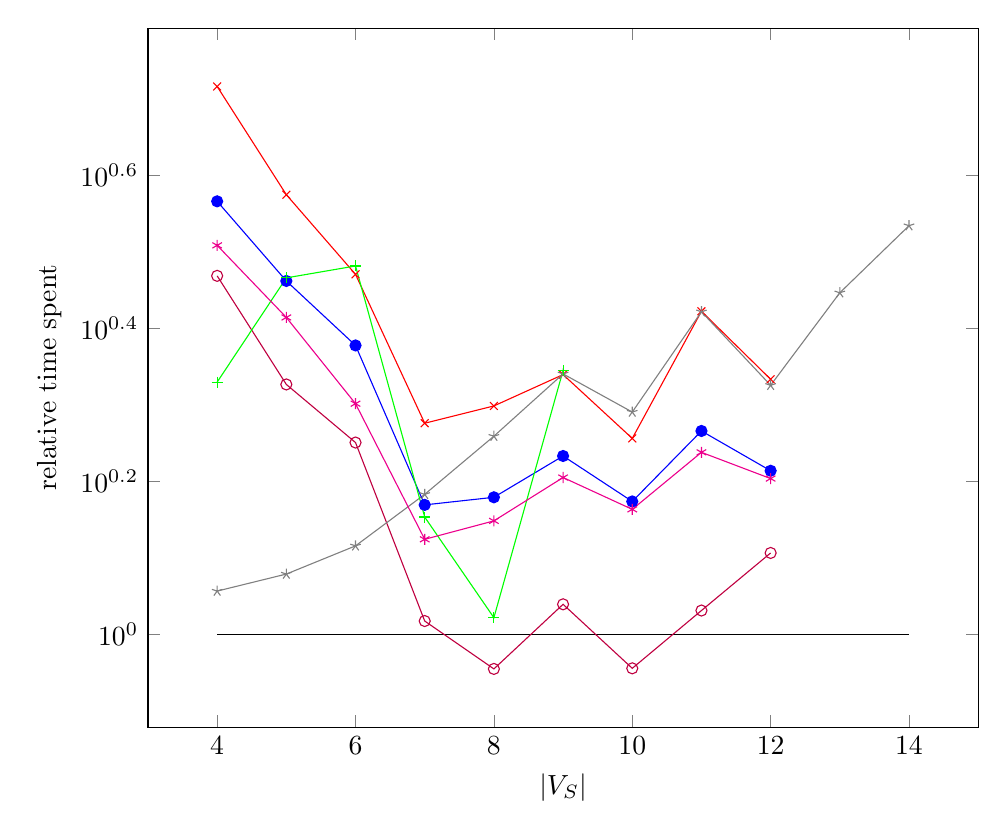
\begin{tikzpicture}
    \begin{axis}[
        xlabel=$|V_S|$,
        ylabel=relative time spent,
        ymode=log,
        legend style={at={(0.9,0.1)},anchor=south east},
        width=\textwidth,
		y tick label style={/pgf/number format/sci},
    ]
\addplot [mark=none, black] plot coordinates {
        (4,1) (14, 1)};



\addplot[
        mark=x,
        red,
    ] plot coordinates {
        (4,5.202946551261944)
        (5,3.756162046192574)
        (6,2.9549254023879072)
        (7,1.8872742557474473)
        (8,1.9880582223277101)
        (9,2.1847812854733193)
        (10,1.8028559351037163)
        (11,2.6436531391416507)
        (12,2.1539273359082483)
};
%    \addlegendentry{DFS}


\addplot[
        mark=o,
        purple,
    ] plot coordinates {
        (4,2.9414858115997387)
        (5,2.120863031356877)
        (6,1.7804930224229873)
        (7,1.0400701807728874)
        (8,0.9003554054490217)
        (9,1.0937936596519373)
        (10,0.9019831415298204)
        (11,1.0734764108654673)
        (12,1.2767276824510232)
};
%    \addlegendentry{GDFS O IP}


\addplot[
        mark=star,
        gray,
    ] plot coordinates {
        (4,1.1382355278673217)
        (5,1.198063456290179)
        (6,1.3042425098741526)
        (7,1.5233183009320665)
        (8,1.8148828000886499)
        (9,2.189451318312936)
        (10,1.9518249758925157)
        (11,2.639768817120566)
        (12,2.1154918845964863)
        (13,2.7952098947822313)
        (14,3.4210781907374623)
};
%    \addlegendentry{GDFS C}


\addplot[
        mark=*,
        blue,
    ] plot coordinates {
        (4,3.6819210072894446)
        (5,2.896400619358773)
        (6,2.3852188316658136)
        (7,1.4756755823523737)
        (8,1.5098085945063882)
        (9,1.7097753943529064)
        (10,1.490937989140139)
        (11,1.8438583447137513)
        (12,1.635315159939935)
};
%    \addlegendentry{K-Path}


\addplot[
        mark=+,
        green,
    ] plot coordinates {
        (4,2.1359021980392736)
        (5,2.923428609692478)
        (6,3.0304568963312812)
        (7,1.4225695726266137)
        (8,1.0506565420981449)
        (9,2.212314905046649)
};
%    \addlegendentry{CP}


\addplot[
        mark=asterisk,
        magenta,
    ] plot coordinates {
        (4,3.2242822734185275)
        (5,2.5950345747500103)
        (6,2.0014242504647624)
        (7,1.3303134982815363)
        (8,1.4062726411755775)
        (9,1.6024494454371436)
        (10,1.4559250035524376)
        (11,1.7288683972843149)
        (12,1.5973164420401704)
};
%    \addlegendentry{GDFS A IP}

	
    \end{axis}
    \end{tikzpicture}

\caption{parallel}
\label{fig:sub3}
\end{subfigure}
\begin{subfigure} {0.5\linewidth}
\centering

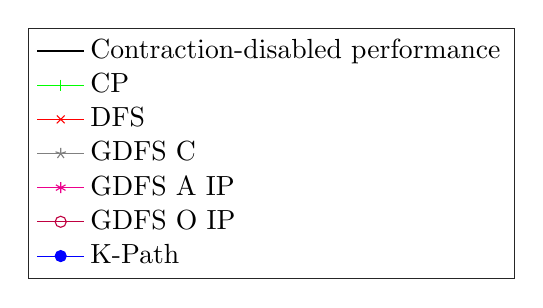
\begin{tikzpicture} 
    \begin{axis}[%
    hide axis,
    xmin=10,
    xmax=50,
    ymin=0,
    ymax=0.4,
    legend style={draw=white!15!black,legend cell align=left}
    ]
	\addlegendimage{black}
    \addlegendentry{Contraction-disabled performance}; 
     
    \addlegendimage{green, mark=+}
    \addlegendentry{CP};
    
    \addlegendimage{red, mark=x}
    \addlegendentry{DFS};
    
    \addlegendimage{gray, mark=star}
    \addlegendentry{GDFS C};
    
    \addlegendimage{magenta, mark=asterisk}
    \addlegendentry{GDFS A IP};
    
    \addlegendimage{purple, mark=o}
    \addlegendentry{GDFS O IP};
    
    \addlegendimage{blue, mark=*}
    \addlegendentry{K-Path};
    
    \end{axis}
\end{tikzpicture}

\end{subfigure}

\caption{Performance of our algorithm with \textbf{ZeroDomain} pruning using \textbf{`N-Filtering'} filtering relative to the performance of the algorithm without pruning. We avoid unnecessarily long paths, do not perform contraction and use the degree-based target graph vertex ordering. Data points above the black reference line denote that the pruning method introduces more delay, and data points below the reference line denote that the pruning method saves time. Note the logarithmic y-axis.}	
\label{fig:zerodomainnfiltering}
\end{figure}

\begin{figure}
\begin{subfigure}{.5\linewidth}
\centering

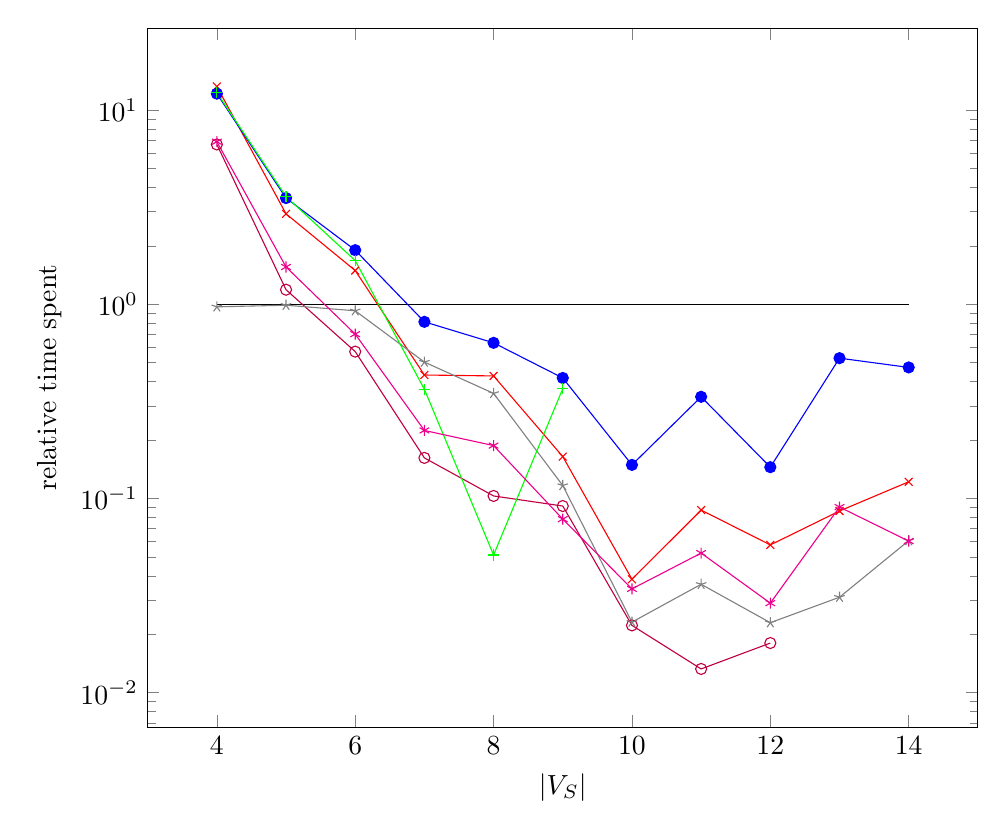
\begin{tikzpicture}
    \begin{axis}[
        xlabel=$|V_S|$,
        ylabel=relative time spent,
        ymode=log,
        legend style={at={(0.9,0.1)},anchor=south east},
        width=\textwidth,
		y tick label style={/pgf/number format/sci},
    ]
\addplot [mark=none, black] plot coordinates {
        (4,1) (14, 1)};

    
	

\addplot[
        mark=x,
        red,
    ] plot coordinates {
        (4,13.228536748772864)
        (5,2.923043265236232)
        (6,1.4918465046685692)
        (7,0.43251422608381307)
        (8,0.4278138461953538)
        (9,0.1643974532055621)
        (10,0.0384235218883735)
        (11,0.08720339702951019)
        (12,0.05769871433439522)
        (13,0.08626318052038495)
        (14,0.12196687793734029)
};
%    \addlegendentry{DFS}


\addplot[
        mark=o,
        purple,
    ] plot coordinates {
        (4,6.652084765296219)
        (5,1.1887666847267304)
        (6,0.5706904469839822)
        (7,0.1619203743990465)
        (8,0.10311284594841497)
        (9,0.09148726872328639)
        (10,0.02222929883828284)
        (11,0.013264269229998682)
        (12,0.01803108077997606)
};
%    \addlegendentry{GDFS O IP}


\addplot[
        mark=star,
        gray,
    ] plot coordinates {
        (4,0.9704520516781957)
        (5,0.9891315449448252)
        (6,0.9259991321183858)
        (7,0.5041146272686665)
        (8,0.34789464456875185)
        (9,0.11668758068736773)
        (10,0.023108258037857765)
        (11,0.03619415549870497)
        (12,0.022948727466520213)
        (13,0.031049777535341994)
        (14,0.06069360971979865)
};
%    \addlegendentry{GDFS C}


\addplot[
        mark=*,
        blue,
    ] plot coordinates {
        (4,12.149621156018027)
        (5,3.524039042210963)
        (6,1.9000540945545796)
        (7,0.8124353858557827)
        (8,0.6333558749485183)
        (9,0.4176331133841372)
        (10,0.1490144308922331)
        (11,0.33404804566046264)
        (12,0.14504260141405623)
        (13,0.5281107544448288)
        (14,0.4731679498288802)
};
%    \addlegendentry{K-Path}


\addplot[
        mark=+,
        green,
    ] plot coordinates {
        (4,12.32026911652997)
        (5,3.58755573944772)
        (6,1.6790110096274846)
        (7,0.36496009660452833)
        (8,0.05120848928373445)
        (9,0.3680142027878651)
};
%    \addlegendentry{CP}


\addplot[
        mark=asterisk,
        magenta,
    ] plot coordinates {
        (4,6.876029334720606)
        (5,1.556841256929411)
        (6,0.7022607700874779)
        (7,0.22412843275278505)
        (8,0.18733394302820017)
        (9,0.07837119253519409)
        (10,0.03427027564684937)
        (11,0.05237617390308613)
        (12,0.028947697493439506)
        (13,0.09038890815957701)
        (14,0.0604047187048502)
};
%    \addlegendentry{GDFS A IP}
  
   
   
   

    \end{axis}
    \end{tikzpicture}


\caption{serial}
\label{fig:sub1}
\end{subfigure}%
\begin{subfigure}{.5\linewidth}
\centering

\begin{tikzpicture}
    \begin{axis}[
        xlabel=$|V_S|$,
        ylabel=relative time spent,
        ymode=log,
        legend style={at={(0.9,0.1)},anchor=south east},
        width=\textwidth,
		y tick label style={/pgf/number format/sci},
    ]
\addplot [mark=none, black] plot coordinates {
        (4,1) (14, 1)};



\addplot[
        mark=x,
        red,
    ] plot coordinates {
        (4,2.5098178926779067)
        (5,0.3542854427484565)
        (6,0.15689010926635982)
        (7,0.035853449977087615)
        (8,0.03523223883158477)
        (9,0.010964699575333747)
        (10,0.0026948377810716018)
        (11,0.0047722023475749165)
        (12,0.003857850717237876)
        (13,0.0047953458790988)
        (14,0.007540380523948009)
};
%    \addlegendentry{DFS}


\addplot[
        mark=o,
        purple,
    ] plot coordinates {
        (4,1.4173101034075382)
        (5,0.1560990152619649)
        (6,0.06332634097438505)
        (7,0.0157805848059952)
        (8,0.009438491623514178)
        (9,0.009468907924155778)
        (10,0.002226287610086919)
        (11,0.001062190759533732)
        (12,0.0015102350651220453)
};
%    \addlegendentry{GDFS O IP}


\addplot[
        mark=star,
        gray,
    ] plot coordinates {
        (4,1.002529859429505)
        (5,0.9854105159518796)
        (6,0.906087246903251)
        (7,0.3747194523117736)
        (8,0.22865139116910282)
        (9,0.060236499046310454)
        (10,0.00840605207241163)
        (11,0.0076697916371780694)
        (12,0.003087366357886867)
        (13,0.003523082302813507)
        (14,0.008191107040264711)
};
%    \addlegendentry{GDFS C}


\addplot[
        mark=*,
        blue,
    ] plot coordinates {
        (4,2.1976489735425813)
        (5,0.3879928825633856)
        (6,0.18575151663949174)
        (7,0.0454443516390044)
        (8,0.044259974145741565)
        (9,0.01934413411554503)
        (10,0.006044262197985706)
        (11,0.007817157760072191)
        (12,0.004400728544806665)
        (13,0.0060658785631791945)
        (14,0.008884903299891778)
};
%    \addlegendentry{K-Path}


\addplot[
        mark=+,
        green,
    ] plot coordinates {
        (4,5.210336306845926)
        (5,1.0605278688734023)
        (6,0.5567531798646309)
        (7,0.17832988212555723)
        (8,0.03032795503714869)
        (9,0.2717523415218701)
};
%    \addlegendentry{CP}


\addplot[
        mark=asterisk,
        magenta,
    ] plot coordinates {
        (4,1.6585184570290825)
        (5,0.24696367603814495)
        (6,0.102320267871855)
        (7,0.025963378720697206)
        (8,0.02247569274863903)
        (9,0.010741035240163122)
        (10,0.003723269579006816)
        (11,0.004340017423267284)
        (12,0.0024617244953977213)
        (13,0.0058187731897781925)
        (14,0.006146499125306626)
};
%    \addlegendentry{GDFS A IP}

	
    \end{axis}
    \end{tikzpicture}

\caption{cached}
\label{fig:sub2}
\end{subfigure}\\[1ex]
\begin{subfigure}{0.5\linewidth}
\centering

\begin{tikzpicture}
    \begin{axis}[
        xlabel=$|V_S|$,
        ylabel=relative time spent,
        ymode=log,
        legend style={at={(0.9,0.1)},anchor=south east},
        width=\textwidth,
		y tick label style={/pgf/number format/sci},
    ]
\addplot [mark=none, black] plot coordinates {
        (4,1) (14, 1)};



\addplot[
        mark=x,
        red,
    ] plot coordinates {
        (4,5.798792679850153)
        (5,3.6257004403518205)
        (6,2.285202142417693)
        (7,0.7445129848838659)
        (8,0.5770188169893984)
        (9,0.3210938826132116)
        (10,0.09131787739629149)
        (11,0.23183733254071692)
        (12,0.13250978599133645)
        (13,0.5487572087616573)
        (14,0.5277236677256409)
};
%    \addlegendentry{DFS}


\addplot[
        mark=o,
        purple,
    ] plot coordinates {
        (4,4.1869563644643)
        (5,1.963563805539359)
        (6,1.1893882290176945)
        (7,0.3225915596294)
        (8,0.196417660886969)
        (9,0.1635088016201688)
        (10,0.06910862435318588)
        (11,0.045930260406800816)
        (12,0.0518105433910061)
};
%    \addlegendentry{GDFS O IP}


\addplot[
        mark=star,
        gray,
    ] plot coordinates {
        (4,1.1043656381381906)
        (5,1.1941146142677403)
        (6,1.1571769969713963)
        (7,0.8519147110949141)
        (8,0.6919890069549386)
        (9,0.30329744854481366)
        (10,0.15267006969696184)
        (11,0.2451122958148758)
        (12,0.12868565849738745)
        (13,0.2468665194487868)
        (14,0.5529525262522433)
};
%    \addlegendentry{GDFS C}


\addplot[
        mark=*,
        blue,
    ] plot coordinates {
        (4,5.036262260510419)
        (5,2.969188933770786)
        (6,1.8496830497872034)
        (7,0.5859718273323613)
        (8,0.43912493395440744)
        (9,0.17191408110115602)
        (10,0.11902810316960899)
        (11,0.2773735237523154)
        (12,0.114049211518233)
        (13,0.438365362697428)
        (14,0.5597451487697097)
};
%    \addlegendentry{K-Path}


\addplot[
        mark=+,
        green,
    ] plot coordinates {
        (4,3.4404078593966663)
        (5,1.4365332891311595)
        (6,0.9370666124380356)
        (7,0.37433319924673136)
        (8,0.04688253357281991)
        (9,0.38910890933793285)
};
%    \addlegendentry{CP}


\addplot[
        mark=asterisk,
        magenta,
    ] plot coordinates {
        (4,4.202135993006676)
        (5,2.5066991227985915)
        (6,1.5392306053079454)
        (7,0.5323918363219251)
        (8,0.41254854061922086)
        (9,0.14979269284608565)
        (10,0.11144241399443222)
        (11,0.1944784771207959)
        (12,0.10750387177004295)
        (13,0.43288906698477536)
        (14,0.37647551651848066)
};
%    \addlegendentry{GDFS A IP}

	
    \end{axis}
    \end{tikzpicture}

\caption{parallel}
\label{fig:sub3}
\end{subfigure}
\begin{subfigure} {0.5\linewidth}
\centering

\begin{tikzpicture} 
    \begin{axis}[%
    hide axis,
    xmin=10,
    xmax=50,
    ymin=0,
    ymax=0.4,
    legend style={draw=white!15!black,legend cell align=left}
    ]
	\addlegendimage{black}
    \addlegendentry{Contraction-disabled performance}; 
     
    \addlegendimage{green, mark=+}
    \addlegendentry{CP};
    
    \addlegendimage{red, mark=x}
    \addlegendentry{DFS};
    
    \addlegendimage{gray, mark=star}
    \addlegendentry{GDFS C};
    
    \addlegendimage{magenta, mark=asterisk}
    \addlegendentry{GDFS A IP};
    
    \addlegendimage{purple, mark=o}
    \addlegendentry{GDFS O IP};
    
    \addlegendimage{blue, mark=*}
    \addlegendentry{K-Path};
    
    \end{axis}
\end{tikzpicture}

\end{subfigure}

\caption{Performance of our algorithm with \textbf{AllDifferent} pruning using \textbf{`Labels and neighbours'} filtering relative to the performance of the algorithm without pruning. We avoid unnecessarily long paths, do not perform contraction and use the degree-based target graph vertex ordering. Data points above the black reference line denote that the pruning method introduces more delay, and data points below the reference line denote that the pruning method saves time. Note the logarithmic y-axis.}	
\label{fig:alldifferentlabelsneighbours}
\end{figure}

\begin{figure}
\begin{subfigure}{.5\linewidth}
\centering

\begin{tikzpicture}
    \begin{axis}[
        xlabel=$|V_S|$,
        ylabel=relative time spent,
        ymode=log,
        legend style={at={(0.9,0.1)},anchor=south east},
        width=\textwidth,
		y tick label style={/pgf/number format/sci},
    ]
\addplot [mark=none, black] plot coordinates {
        (4,1) (14, 1)};

    
   

\addplot[
        mark=x,
        red,
    ] plot coordinates {
        (4,1.0186997833347926)
        (5,1.0232045351532169)
        (6,0.9983077611450746)
        (7,0.9907049947363294)
        (8,0.9986106752415018)
        (9,0.990947997808037)
        (10,0.9833582387420912)
        (11,0.9932844129587108)
        (12,1.0103133629860612)
        (13,0.8895477690842722)
        (14,1.005905267592158)
};
%    \addlegendentry{DFS}


\addplot[
        mark=o,
        purple,
    ] plot coordinates {
        (4,0.9894734471098923)
        (5,0.9968820127769855)
        (6,0.9873225419658352)
        (7,0.9858166681275962)
        (8,0.9904807801930379)
        (9,0.996328709955975)
        (10,0.9809044726735501)
        (11,1.0231407177222254)
        (12,1.0305198945131373)
};
%    \addlegendentry{GDFS O IP}


\addplot[
        mark=star,
        gray,
    ] plot coordinates {
        (4,0.9951732111609184)
        (5,1.005781000751052)
        (6,0.9751302373376524)
        (7,0.9914699309037306)
        (8,1.011362037912515)
        (9,0.9843712362591021)
        (10,0.969402089834849)
        (11,1.0237476067658449)
        (12,1.137294643132325)
        (13,0.9744371513907365)
        (14,0.9802787976693997)
};
%    \addlegendentry{GDFS C}


\addplot[
        mark=*,
        blue,
    ] plot coordinates {
        (4,1.0092933808186613)
        (5,0.7972700999022878)
        (6,0.3874509873372779)
        (7,0.12257854741680918)
        (8,0.11535787568739275)
        (9,0.05517912995992491)
        (10,0.027274471216057083)
        (11,0.09778018796630517)
        (12,0.030614788275003413)
        (13,0.03405177172923535)
        (14,0.17825871037578678)
};
%    \addlegendentry{K-Path}


\addplot[
        mark=+,
        green,
    ] plot coordinates {
        (4,1.0028356859109526)
        (5,0.9904361969575739)
        (6,0.9923987001325429)
        (7,1.0046817332100164)
        (8,0.9858188647918942)
        (9,1.0225063689622522)
};
%    \addlegendentry{CP}


\addplot[
        mark=asterisk,
        magenta,
    ] plot coordinates {
        (4,0.9976349962184932)
        (5,1.0073844165930093)
        (6,0.9981453884688307)
        (7,0.9876792768127225)
        (8,1.0133814377011994)
        (9,0.9520147690376894)
        (10,0.9790339992527488)
        (11,0.9908681483629362)
        (12,1.039543646663335)
        (13,0.9354622696539593)
};
%    \addlegendentry{GDFS A IP}


    \end{axis}
    \end{tikzpicture}


\caption{serial}
\label{fig:sub1}
\end{subfigure}%
\begin{subfigure}{.5\linewidth}
\centering

\begin{tikzpicture}
    \begin{axis}[
        xlabel=$|V_S|$,
        ylabel=relative time spent,
        ymode=log,
        legend style={at={(0.9,0.1)},anchor=south east},
        width=\textwidth,
		y tick label style={/pgf/number format/sci},
    ]
\addplot [mark=none, black] plot coordinates {
        (4,1) (14, 1)};


	

\addplot[
        mark=x,
        red,
    ] plot coordinates {
        (4,0.3083735334423767)
        (5,0.0717983121165574)
        (6,0.02867174161124386)
        (7,0.005353932759145197)
        (8,0.0036018766107605016)
        (9,7.415681550873021E-4)
        (10,2.875045828804046E-4)
        (11,8.113057744684182E-4)
        (12,5.194226380311751E-4)
        (13,1.0634101119189054E-4)
        (14,0.0012129348920926208)
};
%    \addlegendentry{DFS}


\addplot[
        mark=o,
        purple,
    ] plot coordinates {
        (4,0.14979438676735934)
        (5,0.026646145040194358)
        (6,0.010934376147201053)
        (7,0.0021043263511895116)
        (8,9.565212575048943E-4)
        (9,7.087506618627115E-4)
        (10,1.8824424486718616E-4)
        (11,7.522826832084828E-5)
        (12,1.452779418016359E-4)
};
%    \addlegendentry{GDFS O IP}


\addplot[
        mark=star,
        gray,
    ] plot coordinates {
        (4,0.42295684080525053)
        (5,0.7175652095808638)
        (6,0.7072294111057362)
        (7,0.3528461610206276)
        (8,0.1853565026591184)
        (9,0.04895326827559776)
        (10,0.00520061691970819)
        (11,0.004936257731941951)
        (12,0.001192029881315615)
        (13,1.741539188091501E-4)
        (14,0.0014103432783372227)
};
%    \addlegendentry{GDFS C}


\addplot[
        mark=*,
        blue,
    ] plot coordinates {
        (4,0.19863010172526796)
        (5,0.06127991045420755)
        (6,0.02659926027389259)
        (7,0.005297029257396946)
        (8,0.004410971673992958)
        (9,0.0016052971971944885)
        (10,6.884416663917037E-4)
        (11,0.0013566163358025296)
        (12,4.784200055767407E-4)
        (13,2.932097067133155E-4)
        (14,0.0019350025642613788)
};
%    \addlegendentry{K-Path}


\addplot[
        mark=+,
        green,
    ] plot coordinates {
        (4,0.11914885358071148)
        (5,0.08325890354708809)
        (6,0.03669565157098442)
        (7,0.013693561308514623)
        (8,0.0015581760794368682)
        (9,0.021493389120216477)
};
%    \addlegendentry{CP}


\addplot[
        mark=asterisk,
        magenta,
    ] plot coordinates {
        (4,0.167629941635991)
        (5,0.04261429975714803)
        (6,0.01708358998028725)
        (7,0.0034731132709504564)
        (8,0.0024963114206875137)
        (9,8.552890640062261E-4)
        (10,3.776131025451379E-4)
        (11,6.400771612525835E-4)
        (12,3.8951787719665454E-4)
        (13,1.4388024718858805E-4)
        (14,0.0014124109249871175)
};
%    \addlegendentry{GDFS A IP}

	
    \end{axis}
    \end{tikzpicture}

\caption{cached}
\label{fig:sub2}
\end{subfigure}\\[1ex]
\begin{subfigure}{0.5\linewidth}
\centering

\begin{tikzpicture}
    \begin{axis}[
        xlabel=$|V_S|$,
        ylabel=relative time spent,
        ymode=log,
        legend style={at={(0.9,0.1)},anchor=south east},
        width=\textwidth,
		y tick label style={/pgf/number format/sci},
    ]
\addplot [mark=none, black] plot coordinates {
        (4,1) (14, 1)};



\addplot[
        mark=x,
        red,
    ] plot coordinates {
        (4,4.748759594123889)
        (5,2.4295540762796515)
        (6,1.3875324748809377)
        (7,0.3470734386774885)
        (8,0.2952023716844192)
        (9,0.0703958686196079)
        (10,0.03598320014357281)
        (11,0.1183808662884438)
        (12,0.06153628532584232)
        (13,0.03494338911404371)
        (14,0.17160278085125824)
};
%    \addlegendentry{DFS}


\addplot[
        mark=o,
        purple,
    ] plot coordinates {
        (4,2.519594921852216)
        (5,1.1621656243183787)
        (6,0.6397718531506256)
        (7,0.14471136627669023)
        (8,0.07193325075024548)
        (9,0.0605941046017171)
        (10,0.021240531171245025)
        (11,0.018767566782790235)
        (12,0.01758393553367299)
};
%    \addlegendentry{GDFS O IP}


\addplot[
        mark=star,
        gray,
    ] plot coordinates {
        (4,1.2087512038670705)
        (5,1.1995330941514946)
        (6,1.1418853789726933)
        (7,0.5621877889562694)
        (8,0.41022833627945976)
        (9,0.13903913868573037)
        (10,0.04393563116464705)
        (11,0.13498526740722694)
        (12,0.049268960174921994)
        (13,0.030051623484468215)
        (14,0.1635365740440703)
};
%    \addlegendentry{GDFS C}


\addplot[
        mark=*,
        blue,
    ] plot coordinates {
        (4,3.1851467361084174)
        (5,1.8038765225341042)
        (6,1.0539452554077893)
        (7,0.2518608123839957)
        (8,0.18755266523230274)
        (9,0.06769612412018444)
        (10,0.043697519958703857)
        (11,0.1394520374224132)
        (12,0.04337870481595418)
        (13,0.02780400571582131)
        (14,0.11833494711833015)
};
%    \addlegendentry{K-Path}


\addplot[
        mark=+,
        green,
    ] plot coordinates {
        (4,1.0029463243603973)
        (5,0.49661067861132135)
        (6,0.27286554408201)
        (7,0.08419120306502847)
        (8,0.008199948214019814)
        (9,0.07911018316730134)
};
%    \addlegendentry{CP}


\addplot[
        mark=asterisk,
        magenta,
    ] plot coordinates {
        (4,2.92253226917892)
        (5,1.5385463516143498)
        (6,0.8879009793117698)
        (7,0.22506649596273964)
        (8,0.1609402158565465)
        (9,0.06290335332168706)
        (10,0.04548679530232991)
        (11,0.14892017614069342)
        (12,0.04266555665061478)
        (13,0.04753845861304018)
        (14,0.13727172289974587)
};
%    \addlegendentry{GDFS A IP}

	
    \end{axis}
    \end{tikzpicture}

\caption{parallel}
\label{fig:sub3}
\end{subfigure}
\begin{subfigure} {0.5\linewidth}
\centering

\begin{tikzpicture} 
    \begin{axis}[%
    hide axis,
    xmin=10,
    xmax=50,
    ymin=0,
    ymax=0.4,
    legend style={draw=white!15!black,legend cell align=left}
    ]
	\addlegendimage{black}
    \addlegendentry{Contraction-disabled performance}; 
     
    \addlegendimage{green, mark=+}
    \addlegendentry{CP};
    
    \addlegendimage{red, mark=x}
    \addlegendentry{DFS};
    
    \addlegendimage{gray, mark=star}
    \addlegendentry{GDFS C};
    
    \addlegendimage{magenta, mark=asterisk}
    \addlegendentry{GDFS A IP};
    
    \addlegendimage{purple, mark=o}
    \addlegendentry{GDFS O IP};
    
    \addlegendimage{blue, mark=*}
    \addlegendentry{K-Path};
    
    \end{axis}
\end{tikzpicture}

\end{subfigure}

\caption{Performance of our algorithm with \textbf{AllDifferent} pruning using \textbf{`Free neighbours'} filtering relative to the performance of the algorithm without pruning. We avoid unnecessarily long paths, do not perform contraction and use the degree-based target graph vertex ordering. Data points above the black reference line denote that the pruning method introduces more delay, and data points below the reference line denote that the pruning method saves time. Note the logarithmic y-axis.}		
\label{fig:alldifferentunmatched}
\end{figure}

\begin{figure}
\begin{subfigure}{.5\linewidth}
\centering

\begin{tikzpicture}
    \begin{axis}[
        xlabel=$|V_S|$,
        ylabel=relative time spent,
        ymode=log,
        legend style={at={(0.9,0.1)},anchor=south east},
        width=\textwidth,
		y tick label style={/pgf/number format/sci},
    ]
\addplot [mark=none, black] plot coordinates {
        (4,1) (14, 1)};


\addplot[
        mark=x,
        red,
    ] plot coordinates {
        (4,0.9961858191755759)
        (5,1.0059848034836174)
        (6,1.0015623854405225)
        (7,1.0041850516247017)
        (8,0.992834292174954)
        (9,0.9805831782750661)
        (10,1.0131070860496907)
        (11,0.9820629029946675)
        (12,0.9731684469245409)
        (13,0.9978012338195624)
};
%    \addlegendentry{DFS}


\addplot[
        mark=o,
        purple,
    ] plot coordinates {
        (4,0.9991254113598864)
        (5,1.0006304793357408)
        (6,0.9997389129846505)
        (7,1.0024122661594037)
        (8,0.9960200414287358)
        (9,0.9797204693043249)
        (10,1.006094756978359)
        (11,1.0291250941127874)
        (12,1.016228045334132)
};
%    \addlegendentry{GDFS O IP}


\addplot[
        mark=star,
        gray,
    ] plot coordinates {
        (4,1.0059277991423625)
        (5,0.9907814973218768)
        (6,1.0243229749286393)
        (7,1.020235901218478)
        (8,1.028660392466402)
        (9,0.9992951555916159)
        (10,0.9825124885953094)
        (11,0.9832292458336007)
        (12,1.0260311821681063)
        (13,1.1015279814561096)
        (14,1.0152331060942739)
};
%    \addlegendentry{GDFS C}


\addplot[
        mark=*,
        blue,
    ] plot coordinates {
        (4,1.1428023873341047)
        (5,0.8363144144880936)
        (6,0.3883692600044063)
        (7,0.12306323448284873)
        (8,0.11750735154321501)
        (9,0.05546079701782758)
        (10,0.027198570773209862)
        (11,0.09188685028611088)
        (12,0.029187752530780098)
        (13,0.028763961047358233)
        (14,0.13514762161751237)
};
%    \addlegendentry{K-Path}


\addplot[
        mark=+,
        green,
    ] plot coordinates {
        (4,1.003240741424298)
        (5,1.0007002255334068)
        (6,0.9998134962523451)
        (7,0.9954368842322697)
        (8,0.9901138150986978)
        (9,1.0994301778756659)
};
%    \addlegendentry{CP}


\addplot[
        mark=asterisk,
        magenta,
    ] plot coordinates {
        (4,1.012208101549136)
        (5,1.004540535143729)
        (6,1.006238667112502)
        (7,0.9987787321626621)
        (8,0.9857632446293185)
        (9,1.00045313105658)
        (10,0.9800057859162024)
        (11,1.0071924078562504)
        (12,1.05284665552656)
        (13,1.0473613609958743)
};
%    \addlegendentry{GDFS A IP}

 

    \end{axis}
    \end{tikzpicture}


\caption{serial}
\label{fig:sub1}
\end{subfigure}%
\begin{subfigure}{.5\linewidth}
\centering

\begin{tikzpicture}
        \begin{axis}[
        xlabel=$|V_S|$,
        ylabel=relative time spent,
        ymode=log,
        legend style={at={(0.9,0.1)},anchor=south east},
        width=\textwidth,
		y tick label style={/pgf/number format/sci},
    ]
\addplot [mark=none, black] plot coordinates {
        (4,1) (14, 1)};

	

\addplot[
        mark=x,
        red,
    ] plot coordinates {
        (4,0.28797946415268216)
        (5,0.07651582579324001)
        (6,0.0304666091954765)
        (7,0.005338589440600172)
        (8,0.0038271200815995776)
        (9,7.967244945263907E-4)
        (10,3.0777658183211987E-4)
        (11,7.316319897914259E-4)
        (12,3.4267518525965546E-4)
        (13,1.0795184070755415E-4)
        (14,7.623451601108666E-4)
};
%    \addlegendentry{DFS}


\addplot[
        mark=o,
        purple,
    ] plot coordinates {
        (4,0.15049515351200515)
        (5,0.028888664846084877)
        (6,0.011744849761370135)
        (7,0.0021597185405343167)
        (8,9.451813259466757E-4)
        (9,7.108005706910614E-4)
        (10,1.2347079460250932E-4)
        (11,9.95681216803268E-5)
        (12,1.6636754548371435E-4)
};
%    \addlegendentry{GDFS O IP}


\addplot[
        mark=star,
        gray,
    ] plot coordinates {
        (4,0.4261569662504955)
        (5,0.6566221486790923)
        (6,0.5577822930842058)
        (7,0.3218592258892897)
        (8,0.18912427965228307)
        (9,0.047186436624101824)
        (10,0.006370129606168451)
        (11,0.0012501421281951863)
        (12,0.001428282896214883)
        (13,1.4047897093971695E-4)
        (14,0.0012339028104273453)
};
%    \addlegendentry{GDFS C}


\addplot[
        mark=*,
        blue,
    ] plot coordinates {
        (4,0.19921889891317368)
        (5,0.06836073093997885)
        (6,0.02840796237713794)
        (7,0.005614455272937469)
        (8,0.004672519202561842)
        (9,0.001547859891521619)
        (10,4.269626026969231E-4)
        (11,0.0011715845435014138)
        (12,5.118613622622226E-4)
        (13,3.9341491023758834E-4)
        (14,0.0011207533086203814)
};
%    \addlegendentry{K-Path}


\addplot[
        mark=+,
        green,
    ] plot coordinates {
        (4,0.12065618974765957)
        (5,0.08159990593923339)
        (6,0.03466025100832615)
        (7,0.013147623578769863)
        (8,0.0017371671223744833)
        (9,0.03084198984204367)
};
%    \addlegendentry{CP}


\addplot[
        mark=asterisk,
        magenta,
    ] plot coordinates {
        (4,0.1784159199448806)
        (5,0.04687838004113365)
        (6,0.019250300262524056)
        (7,0.003877520221788777)
        (8,0.0028497378324052747)
        (9,9.238160016552532E-4)
        (10,3.1576391186238784E-4)
        (11,7.994265736620543E-4)
        (12,3.8594286429616265E-4)
        (13,1.6073739183641855E-4)
        (14,6.707501289580087E-4)
};
%    \addlegendentry{GDFS A IP}

	
    \end{axis}
    \end{tikzpicture}

\caption{cached}
\label{fig:sub2}
\end{subfigure}\\[1ex]
\begin{subfigure}{0.5\linewidth}
\centering

\begin{tikzpicture}
    \begin{axis}[
        xlabel=$|V_S|$,
        ylabel=relative time spent,
        ymode=log,
        legend style={at={(0.9,0.1)},anchor=south east},
        width=\textwidth,
		y tick label style={/pgf/number format/sci},
    ]
\addplot [mark=none, black] plot coordinates {
        (4,1) (14, 1)};


\addplot[
        mark=x,
        red,
    ] plot coordinates {
        (4,3.9129439575545435)
        (5,2.273222753540935)
        (6,1.3358829167973778)
        (7,0.3060292392269831)
        (8,0.27310812493561054)
        (9,0.08483478635788988)
        (10,0.03220002459721227)
        (11,0.10965821877648596)
        (12,0.05238033266084752)
        (13,0.02720606162053374)
        (14,0.12326343330507006)
};
%    \addlegendentry{DFS}


\addplot[
        mark=o,
        purple,
    ] plot coordinates {
        (4,2.4370501012142824)
        (5,1.0568408408459573)
        (6,0.5835598718338068)
        (7,0.13489675395340783)
        (8,0.06428756573066419)
        (9,0.04934951432140211)
        (10,0.01966479503287344)
        (11,0.018929462405664066)
        (12,0.01752267312020006)
};
%    \addlegendentry{GDFS O IP}


\addplot[
        mark=star,
        gray,
    ] plot coordinates {
        (4,1.5119445424232758)
        (5,1.6205884547090093)
        (6,1.4772813435520415)
        (7,0.6353071431015811)
        (8,0.41070975405654797)
        (9,0.13580170759422583)
        (10,0.03828888536206054)
        (11,0.10934140002182946)
        (12,0.0411628308005999)
        (13,0.024956633661657346)
        (14,0.16725255988991872)
};
%    \addlegendentry{GDFS C}


\addplot[
        mark=*,
        blue,
    ] plot coordinates {
        (4,2.9292287176662284)
        (5,1.7085776030673339)
        (6,1.018144876988824)
        (7,0.22453968974110117)
        (8,0.18160614741581238)
        (9,0.06924099256113281)
        (10,0.04038867770933918)
        (11,0.12581531378172073)
        (12,0.04559446907724363)
        (13,0.04043070416472683)
        (14,0.10402774643082491)
};
%    \addlegendentry{K-Path}


\addplot[
        mark=+,
        green,
    ] plot coordinates {
        (4,0.9551312671725737)
        (5,0.46672792929157314)
        (6,0.25108420813909216)
        (7,0.09084564408241347)
        (8,0.009073128728892876)
        (9,0.09911792703918121)
};
%    \addlegendentry{CP}


\addplot[
        mark=asterisk,
        magenta,
    ] plot coordinates {
        (4,2.6450452172441703)
        (5,1.466590988138647)
        (6,0.8335425887125216)
        (7,0.20265590602141004)
        (8,0.14860699155681456)
        (9,0.058559839513090184)
        (10,0.03613722819737897)
        (11,0.1373961637320401)
        (12,0.039138601300597764)
        (13,0.04064207588686031)
        (14,0.09797085693851426)
};
%    \addlegendentry{GDFS A IP}

	
    \end{axis}
    \end{tikzpicture}

\caption{parallel}
\label{fig:sub3}
\end{subfigure}
\begin{subfigure} {0.5\linewidth}
\centering

\begin{tikzpicture} 
    \begin{axis}[%
    hide axis,
    xmin=10,
    xmax=50,
    ymin=0,
    ymax=0.4,
    legend style={draw=white!15!black,legend cell align=left}
    ]
	\addlegendimage{black}
    \addlegendentry{Contraction-disabled performance}; 
     
    \addlegendimage{green, mark=+}
    \addlegendentry{CP};
    
    \addlegendimage{red, mark=x}
    \addlegendentry{DFS};
    
    \addlegendimage{gray, mark=star}
    \addlegendentry{GDFS C};
    
    \addlegendimage{magenta, mark=asterisk}
    \addlegendentry{GDFS A IP};
    
    \addlegendimage{purple, mark=o}
    \addlegendentry{GDFS O IP};
    
    \addlegendimage{blue, mark=*}
    \addlegendentry{K-Path};
    
    \end{axis}
\end{tikzpicture}

\end{subfigure}

\caption{Performance of our algorithm with \textbf{AllDifferent} pruning using \textbf{`M-filtering'} filtering relative to the performance of the algorithm without pruning. We avoid unnecessarily long paths, do not perform contraction and use the degree-based target graph vertex ordering. Data points above the black reference line denote that the pruning method introduces more delay, and data points below the reference line denote that the pruning method saves time. Note the logarithmic y-axis.}		
\label{fig:alldifferentMfiltering}
\end{figure}

\begin{figure}
\begin{subfigure}{.5\linewidth}
\centering

\begin{tikzpicture}
    \begin{axis}[
        xlabel=$|V_S|$,
        ylabel=relative time spent,
        ymode=log,
        legend style={at={(0.9,0.1)},anchor=south east},
        width=\textwidth,
		y tick label style={/pgf/number format/sci},
    ]
\addplot [mark=none, black] plot coordinates {
        (4,1) (14,1)};

    
   

\addplot[
        mark=x,
        red,
    ] plot coordinates {
        (4,0.9676950624676575)
        (5,0.9988894067222226)
        (6,1.0005763973495974)
        (7,1.0012522076540606)
        (8,1.0107283953513952)
        (9,0.9599448767629568)
        (10,1.0347901686226628)
        (11,1.0103410684538925)
        (12,1.0255798438058548)
        (13,0.9056614547818025)
        (14,0.9698848854871277)
};
%    \addlegendentry{DFS}


\addplot[
        mark=o,
        purple,
    ] plot coordinates {
        (4,1.0094137822150915)
        (5,1.0030498615384387)
        (6,0.996041126474167)
        (7,1.0014862936237205)
        (8,1.006913278037861)
        (9,0.9865779317721944)
        (10,0.973979329150809)
        (11,1.0085691395261733)
        (12,1.012790208560442)
};
%    \addlegendentry{GDFS O IP}


\addplot[
        mark=star,
        gray,
    ] plot coordinates {
        (4,1.0410716738680912)
        (5,1.008890447711797)
        (6,0.9929773547796908)
        (7,1.0053072922093342)
        (8,1.0058758041034963)
        (9,1.0067325036708086)
        (10,1.0080505476192445)
        (11,0.9598589720985476)
        (12,0.9601497898994072)
        (13,1.05397295806311)
        (14,0.9852887590169078)
};
%    \addlegendentry{GDFS C}


\addplot[
        mark=*,
        blue,
    ] plot coordinates {
        (4,1.5970781583369893)
        (5,1.0429950475098546)
        (6,0.5642557451473594)
        (7,0.19187744681948582)
        (8,0.16271009963035188)
        (9,0.0715045220335021)
        (10,0.046728031478004195)
        (11,0.10603600840907235)
        (12,0.03729878780829776)
        (13,0.04017799631235486)
        (14,0.1473463960242647)
};
%    \addlegendentry{K-Path}


\addplot[
        mark=+,
        green,
    ] plot coordinates {
        (4,1.0136425248501462)
        (5,1.0007246262269673)
        (6,0.9976668304761186)
        (7,0.9885168025956491)
        (8,1.0110440897106538)
        (9,1.0265495887464324)
};
%    \addlegendentry{CP}


\addplot[
        mark=asterisk,
        magenta,
    ] plot coordinates {
        (4,0.9925924238577477)
        (5,0.9932698347961497)
        (6,1.002644406556925)
        (7,1.0082608252132723)
        (8,1.0002625398016867)
        (9,0.9673299243637845)
        (10,1.0357874894276926)
        (11,1.0267563810636593)
        (12,1.015497232110587)
        (13,1.0002726400770723)
};
%    \addlegendentry{GDFS A IP}


    \end{axis}
    \end{tikzpicture}


\caption{serial}
\label{fig:sub1}
\end{subfigure}%
\begin{subfigure}{.5\linewidth}
\centering

\begin{tikzpicture}
    \begin{axis}[
        xlabel=$|V_S|$,
        ylabel=relative time spent,
        ymode=log,
        legend style={at={(0.9,0.1)},anchor=south east},
        width=\textwidth,
		y tick label style={/pgf/number format/sci},
    ]
\addplot [mark=none, black] plot coordinates {
        (4,1) (14, 1)};


	

\addplot[
        mark=x,
        red,
    ] plot coordinates {
        (4,0.3693236491674021)
        (5,0.08662776836402786)
        (6,0.03543362590095955)
        (7,0.006177208718380012)
        (8,0.004144420637945623)
        (9,9.354448414969907E-4)
        (10,3.1869623984615014E-4)
        (11,6.942032052866809E-4)
        (12,4.92629092351704E-4)
        (13,1.236654683463012E-4)
        (14,8.145275946982444E-4)
};
%    \addlegendentry{DFS}


\addplot[
        mark=o,
        purple,
    ] plot coordinates {
        (4,0.18371858693151044)
        (5,0.030401734904650368)
        (6,0.012976374788824407)
        (7,0.002405059847648494)
        (8,9.138047489324341E-4)
        (9,7.701810544392673E-4)
        (10,1.3963369512837165E-4)
        (11,8.996547626749507E-5)
        (12,1.4807292756369161E-4)
};
%    \addlegendentry{GDFS O IP}


\addplot[
        mark=star,
        gray,
    ] plot coordinates {
        (4,0.3196707718030456)
        (5,0.4119004671239389)
        (6,0.3945929975644642)
        (7,0.3597088103007954)
        (8,0.18276813544122272)
        (9,0.053068079095563214)
        (10,0.005540376398996627)
        (11,0.005146721461176784)
        (12,0.0033440271263982524)
        (13,1.5787860587113123E-4)
        (14,0.0012506224638044738)
};
%    \addlegendentry{GDFS C}


\addplot[
        mark=*,
        blue,
    ] plot coordinates {
        (4,0.25280034627371606)
        (5,0.06370234194664193)
        (6,0.02923362323560863)
        (7,0.005458665126135687)
        (8,0.004121676516919193)
        (9,0.0013445510878975497)
        (10,3.8782765857092727E-4)
        (11,9.762077809364333E-4)
        (12,3.7839915244086697E-4)
        (13,2.0719974514915585E-4)
        (14,9.972179281756421E-4)
};
%    \addlegendentry{K-Path}


\addplot[
        mark=+,
        green,
    ] plot coordinates {
        (4,0.09603666224543228)
        (5,0.045282268345635424)
        (6,0.022983591743019782)
        (7,0.009213437075401898)
        (8,0.0010550572324501406)
        (9,0.020807435412101838)
};
%    \addlegendentry{CP}


\addplot[
        mark=asterisk,
        magenta,
    ] plot coordinates {
        (4,0.20290440891034733)
        (5,0.04978550630960299)
        (6,0.020792134867174017)
        (7,0.004179165900801252)
        (8,0.0031241683734722914)
        (9,9.241937127778543E-4)
        (10,3.455504261065112E-4)
        (11,7.470512282303776E-4)
        (12,2.9066662540455646E-4)
        (13,1.0982181047392015E-4)
        (14,7.830472075457395E-4)
};
%    \addlegendentry{GDFS A IP}

	
    \end{axis}
    \end{tikzpicture}

\caption{cached}
\label{fig:sub2}
\end{subfigure}\\[1ex]
\begin{subfigure}{0.5\linewidth}
\centering

\begin{tikzpicture}
    \begin{axis}[
        xlabel=$|V_S|$,
        ylabel=relative time spent,
        ymode=log,
        legend style={at={(0.9,0.1)},anchor=south east},
        width=\textwidth,
		y tick label style={/pgf/number format/sci},
    ]
\addplot [mark=none, black] plot coordinates {
        (4,1) (14, 1)};



\addplot[
        mark=x,
        red,
    ] plot coordinates {
        (4,5.1345832619134315)
        (5,3.100425102383263)
        (6,1.8852096728253702)
        (7,0.4708800143588947)
        (8,0.41618998589925804)
        (9,0.1027206607222183)
        (10,0.059163250604911566)
        (11,0.18439902177485434)
        (12,0.08285693958613916)
        (13,0.07033185960559696)
        (14,0.19062567426078747)
};
%    \addlegendentry{DFS}


\addplot[
        mark=o,
        purple,
    ] plot coordinates {
        (4,2.774994132451617)
        (5,1.3574173398460796)
        (6,0.851912409726081)
        (7,0.1991114927169909)
        (8,0.09455509094612868)
        (9,0.0818077201557178)
        (10,0.03242406032574496)
        (11,0.03040410201940047)
        (12,0.028403050719100542)
};
%    \addlegendentry{GDFS O IP}


\addplot[
        mark=star,
        gray,
    ] plot coordinates {
        (4,1.0909185494014733)
        (5,1.182187346908493)
        (6,1.1328378765879803)
        (7,0.7233308955429363)
        (8,0.5086224425944339)
        (9,0.18394420655553456)
        (10,0.07234125105236022)
        (11,0.20874358974197005)
        (12,0.07136307095042382)
        (13,0.05297957121058816)
        (14,0.23772304496314955)
};
%    \addlegendentry{GDFS C}


\addplot[
        mark=*,
        blue,
    ] plot coordinates {
        (4,3.8970195420742755)
        (5,2.2939604690071147)
        (6,1.481691252343444)
        (7,0.35686658381717284)
        (8,0.2762673233671855)
        (9,0.10864296003618246)
        (10,0.06803550925927393)
        (11,0.22460191218117787)
        (12,0.07692161844416523)
        (13,0.06719809667315302)
        (14,0.20985511070050933)
};
%    \addlegendentry{K-Path}


\addplot[
        mark=+,
        green,
    ] plot coordinates {
        (4,1.0848428708890463)
        (5,0.4591837362904758)
        (6,0.26321451914524563)
        (7,0.0809303914306656)
        (8,0.007455460280270221)
        (9,0.07164052373260954)
};
%    \addlegendentry{CP}


\addplot[
        mark=asterisk,
        magenta,
    ] plot coordinates {
        (4,2.981403961199849)
        (5,2.00009795935702)
        (6,1.168640642979861)
        (7,0.31603922204888457)
        (8,0.22195394127915336)
        (9,0.08780473818064749)
        (10,0.06100100883433479)
        (11,0.23639828072837477)
        (12,0.06149452415020673)
        (13,0.09018840369746495)
        (14,0.24168554995385316)
};
%    \addlegendentry{GDFS A IP}

	
    \end{axis}
    \end{tikzpicture}

\caption{parallel}
\label{fig:sub3}
\end{subfigure}
\begin{subfigure} {0.5\linewidth}
\centering

\begin{tikzpicture} 
    \begin{axis}[%
    hide axis,
    xmin=10,
    xmax=50,
    ymin=0,
    ymax=0.4,
    legend style={draw=white!15!black,legend cell align=left}
    ]
	\addlegendimage{black}
    \addlegendentry{Contraction-disabled performance}; 
     
    \addlegendimage{green, mark=+}
    \addlegendentry{CP};
    
    \addlegendimage{red, mark=x}
    \addlegendentry{DFS};
    
    \addlegendimage{gray, mark=star}
    \addlegendentry{GDFS C};
    
    \addlegendimage{magenta, mark=asterisk}
    \addlegendentry{GDFS A IP};
    
    \addlegendimage{purple, mark=o}
    \addlegendentry{GDFS O IP};
    
    \addlegendimage{blue, mark=*}
    \addlegendentry{K-Path};
    
    \end{axis}
\end{tikzpicture}

\end{subfigure}

\caption{Performance of our algorithm with \textbf{AllDifferent} pruning using \textbf{`N-filtering'} filtering relative to the performance of the algorithm without pruning. We avoid unnecessarily long paths, do not perform contraction and use the degree-based target graph vertex ordering. Data points above the black reference line denote that the pruning method introduces more delay, and data points below the reference line denote that the pruning method saves time. Note the logarithmic y-axis.}		
\label{fig:alldifferentNfiltering}
\end{figure}






\section{Software design}
\subsection{Architecture}
\subsection{Manual}
\chapter{Conclusion}
\begin{minipage}{\textwidth}
In this research, we aimed to investigate how to map a configuration for a virtual FPGA to one usable for a real-life concrete FPGA. One goal of such an emulation is allowing college students to learn about the FPGA compilation and synthesis process using a simple, easy-to-understand FPGA but still running their configurations on real hardware. Moreover, this problem fits within the greater research area of partial FPGA compilation: abtracting parts of an FPGA away such that they may be used for other purposes.  We reduced this emulation problem to `subgraph homeomorphism', an NP-complete graph problem. This is a problem for which several algorithms existed, but none met the space- and computational requirements needed for the scale of the inputs (graphs of the FPGAs). Because of this, we decided to adapt an algorithm such that it does meet the requirements. One of these algorithms was ndsh2: an algorithm that has minimum exponential space requirements. We adapted ndsh2, to a variant that only has polynomial space requirements (or even linear under some settings). To improve our chances of finding subgraph homeomorphisms, we added several optimisations: refusing paths using unnecessarily many FPGA resources, contraction, alldifferent pruning and various ways to order vertices in either graph. We found that each of these optimisations (except the target graph vertex ordering) may reduce the time spent on finding homeomorphisms.

We benchmarked the performance of this algorithm with optimal settings and extrapolate that the business case will take approximately {\color{red} TODO} time. {\color{red} TODO: make conclusion about applicabilty} Since we were not able to find a subgraph homeomorphism between the FPGAs of the business case yet, we are unable to conclude how many resources of the concrete FPGA are needed for each virtual logic case. Based on our models, however we can deduce that at best two virtual logic cells fit on each ECP5 logic tile.

The algorithm we proposed is also applicable for graphs outside of the FPGA emulation domain. While the conclusions we make from our experiments are based on graphs representing FPGAs with their structure, our software toolbox with individually changeable settings allows for benchmarks on other graphs as well. Our software (or other software created with our methodology) can be used to establish the appriopriate configuration for any other domain reducable to subgraph homeomorphism.

Based on this algorithm, we establish a methodology to obtain a mapping for linear time emulation of virtual FPGAs on concrete FPGAs.
\end{minipage}
\chapter{Discussion}
From our experiments, we found that in-place depth first search path iteration is (of the methods compared) the most efficient path iteration method to replace Xiao's structure with precomputed paths for our business case. We could not find enough data to make conclusions on how memory usage scales with each path iteration method; however, all path iteration methods (except for control point iteration) seem to scale approximately equally within our graph size range.

Our experiments show that the GreatestConstrainedFirst source graph vertex ordering from RI-DS \cite{RIalgorithm} is indeed more efficient than the assumed random ordering of Xiao's algorithm. Moreover, the experiments show that ordering target vertices by degree introduced by Glasgow \cite{McCreesh2015} is on average more efficient than the assumed random ordering of Xiao's algorithm or the distance-based ordering we introduced.

We compared each of our 24 pruning methods and conclude that cached AllDifferent pruning with N-filtering is the most computationally effective pruning method for our business case. This is partly in line with Xiao's algorithm, which uses cached ZeroDomain pruning with N-filtering.

With regards to space usage, we see no reason to prefer one option over the other: the effect of the pruner choice has a minor effect on space usage, likely unnoticeable in a business environment.

For applications of our algorithm outside of FPGA emulation, different settings may yield better performance. Our test cases are specifically designed to represent graphs that adhere to our FPGA graph model, and may have properties that graphs from a different domain do not have. Therefore, verifying the appropriate settings for a different business case is adviseable if computational requirements are relevant.

{\color{red} TODO: extrapolate how much time is needed for business case. Is this acceptable?}

A disadvantage of our approach is that it requires modelling the virtual FPGA into hardware components (wires, transistors et cetera). Some models might result in subgraph homeomorphisms being found, while some models might not. A possible technique to remedy this is to attempt several different models simultaneously, using heuristics to estimate the likeliness of each model to result in a subgraph homeomorphism being found.

Even then, a subgraph homeomorphism may not be found even though a theoretical emulation exists: our methodology only looks for emulation of individual virtual components by individual concrete components and does not look for solutions where sets of virtual components are emulated by sets of virtual concrete components that may be composed of different component types. However, there might not be a solution to this: in general, an emulation mapping should map each possible function on the virtual FPGA to a semantically equivalent function on the concrete FPGA. Deciding whether two functions are semantically equivalent is an undecideable problem in general, only limited by the size of the FPGA. It is thus appriopriate to use a methodology that is most likely to find an emulation mapping where one exists, for which we provide a candidate with our methodology.
\chapter{Future Research}

\begin{enumerate}
\item concurrent tree exploration
\item Backmarking and backjumping
\item choose target graph vertices based on some location heuristic, e.g. tiles
\item use hierachy: e.g. when a component has been matched with some pattern Q, immediately match the next component with an isomorphic pattern Q', allowing for backtracking
\end{enumerate}

\begin{appendices}

\section{History of subgraph isomorphism algorithms}
\label{app:algorithmHistory}
\adjincludegraphics[width=\textwidth, trim={0 {.555\height} 0 0},clip]{images/algorithmhistory.png}
\adjincludegraphics[width=\textwidth, trim={0 0 0 {.445\height}},clip]{images/algorithmhistory.png}
\section{Examples of path iterators}
\label{app:pathIteratorExamples}
%-----------------
%K-PATH EXAMPLE
%-----------------
\begin{figure}[ht]
\begin{subfigure}{.5\textwidth}
  \centering
  % include first image
\includegraphics[width=0.8\linewidth]{images/pathiterators/examples-kpath-1.png}
  \caption{First path}
\end{subfigure}
\begin{subfigure}{.5\textwidth}
  \centering
  % include second image
\includegraphics[width=0.8\linewidth]{images/pathiterators/examples-kpath-2.png}
  \caption{Second path}
\end{subfigure}
\caption{The first two iterations of the K-path path iterator in a square graph. This example is unaffected by ``refusing longer paths".}
\label{fig:pathexamples-kpath}
\end{figure}

%-----------------
%DFS EXAMPLE
%-----------------
\begin{figure}[ht]
\begin{subfigure}{.5\textwidth}
  \centering
  % include first image
\includegraphics[width=0.8\linewidth]{images/pathiterators/examples-DFS-1.png}
  \caption{First path}
\end{subfigure}
\begin{subfigure}{.5\textwidth}
  \centering
  % include second image
\includegraphics[width=0.8\linewidth]{images/pathiterators/examples-DFS-2.png}
  \caption{Second path}
\end{subfigure}

\begin{subfigure}{.5\textwidth}
  \centering
  % include second image
\includegraphics[width=0.8\linewidth]{images/pathiterators/examples-DFS-1-RLP.png}
  \caption{First path (refusing longer paths)}
\end{subfigure}
\begin{subfigure}{.5\textwidth}
  \centering
  % include second image
\includegraphics[width=0.8\linewidth]{images/pathiterators/examples-DFS-2-RLP.png}
  \caption{Second path (refusing longer paths)}
\end{subfigure}
\caption{The first two iterations of the DFS path iterator in a square graph.}
\label{fig:pathexamples-dfs}
\end{figure}



%-----------------
%GREEDY DFS EXAMPLE
%-----------------
\begin{figure}[ht]
\begin{subfigure}{.5\textwidth}
  \centering
\includegraphics[width=0.8\linewidth]{images/pathiterators/examples-Greedy DFS-1.png}
  \caption{First path}
\end{subfigure}
\begin{subfigure}{.5\textwidth}
  \centering
\includegraphics[width=0.8\linewidth]{images/pathiterators/examples-Greedy DFS-2.png}
  \caption{Second path}
\end{subfigure}

\begin{subfigure}{.5\textwidth}
  \centering
\includegraphics[width=0.8\linewidth]{images/pathiterators/examples-Greedy DFS-1.png}
  \caption{First path (refusing longer paths)}
\end{subfigure}
\begin{subfigure}{.5\textwidth}
  \centering
\includegraphics[width=0.8\linewidth]{images/pathiterators/examples-Greedy DFS-reflongerpaths.png}
  \caption{Second path (refusing longer paths)}
\end{subfigure}
\caption{The first two iterations of the greedy DFS path iterator in a square graph.}
\label{fig:pathexamples-greedydfs}
\end{figure}

%-----------------
%CONTROL POINT EXAMPLE
%-----------------
\begin{figure}[ht]
\begin{subfigure}{.5\textwidth}
  \centering
  % include first image
\includegraphics[width=0.8\linewidth]{images/pathiterators/examples-Control point-1.png}
  \caption{First path (0 control points)}
\end{subfigure}
\begin{subfigure}{.5\textwidth}
  \centering
  % include second image
\includegraphics[width=0.8\linewidth]{images/pathiterators/examples-Control point-2.png}
  \caption{Second path (1 control point)}
\end{subfigure}
\caption{The first two iterations of the control point path iterator in a square graph. This example is unaffected by ``refusing longer paths".}
\label{fig:pathexamples-controlpoint}
\end{figure}
\section{Proof: contraction preserves subgraph homeomorphism}
\label{proof:contractionHomeo}
\begin{proof}

Let $\mathit{vcontract}_{S' \to S}$ and $\mathit{econtract}_{S' \to S}$ be the (injective) vertex-to-vertex mapping and (injective) edge-to-path mapping from the contracted graph $S_{cont}$ to $S$, respectively, and let $(\mathit{vmap}_{S \to T}, \mathit{emap}_{S \to T})$ be some vertex disjoint subgraph homeomorphism from $S$ to $T$, respectively.

We then construct a vertex-to-vertex mapping $\mathit{vmap}_{S' \to T}$ by mapping each vertex $v \in V_{S'}$ to $\mathit{vmap}_{S \to T}(\mathit{vcontract}_{S' \to S}(v))$. Recall from the definition of subgraph homeomorphism that $\forall s \in V_S . L_S(s) \subseteq L_T(\mathit{vmap}_{S to T}(s))$. This holds for $S$ and $T$ since we assumed a subgraph homeomorphism existed between the two.

Since for every vertex $v \in V_{S'}$ we have $\mathit{vcontract}_{S' \to S}(v) \in V_s$, it also holds that $\forall s' \in V_{S'} . L_S(\mathit{vcontract}_{S' \to S}(s')) \subseteq L_T(\mathit{vmap}_{S \to T}(\mathit{vcontract}_{S' \to S}(s')))$. Moreover, since labels of remaining vertices are preserved through contraction, we have $\forall v \in V_{S'}.L_{S'}(v)=L_S(\mathit{vcontract}_{S' \to S}(v))$. Therefore, it holds that: $\forall s' \in V_{S'} . L_{S'}(s') \subseteq L_T(\mathit{vmap}_{S \to T}(\mathit{vcontract}_{S' \to S}(s')))$. Therefore, this vertex-to-vertex mapping satisfies the first prequisite out of three for vertex disjoint subgraph homeomorphism.

We then construct an edge-to-path mapping $\mathit{emap}_{S' \to T}$. For each edge $(u, v) \in E_{S'}$, we take the edges of the path $\mathit{econtract}_{S' \to S}((u, v))$ and concatenate the edges of the corresponding paths in $T$ to obtain a new path $p'$. We then add $((u, v), p')$ to $\mathit{emap}_{S' \to T}$. Recall from the definition of subgraph homeomorphism that:

\begin{tabular}{ll}
$\forall(s_1, s_2)\in E_S .$&$ \mathit{first}(\mathit{emap}_{S \to T}(s_1, s_2))=\mathit{vmap}_{S \to T}(s_1)\land$\\
&$\mathit{last}(\mathit{emap}_{S \to T}(s_1, s_2))=\mathit{vmap}_{S \to T}(s_2)$.
\end{tabular}

Applying this formula to two consecutive edges allow us to conclude:

\begin{tabular}{ll}
$\forall(s_1, s_2), (s_2, s_3)\in E_S . $&$\mathit{first}(\mathit{emap}_{S \to T}(s_1, s_2))=\mathit{vmap}_{S \to T}(s_1)\land$\\
&$\mathit{last}(\mathit{emap}_{S \to T}(s_2, s_3))=\mathit{vmap}_{S \to T}(s_3)$. 
\end{tabular}

And similarly for more concatenated edges. Choosing the edge sequences such that each edge sequence in $S$ corresponds to a single edge in $S'$ gives us:

\begin{tabular}{ll}
$\forall(s'_1, s'_2)\in E_{S'} . $&$\mathit{first}(\mathit{emap}_{S \to T}(\mathit{firstEdge}(\mathit{econtract}(s'_1, s'_2))))=\mathit{vmap}_{S \to T}(\mathit{vcontract}(s_1))\land$\\
&$\mathit{last}(\mathit{emap}_{S \to T}(\mathit{lastEdge}(\mathit{econtract}(s'_1, s'_2))))=\mathit{vmap}_{S \to T}(\mathit{vcontract}(s'_2))$
\end{tabular}

which shows we satisfy the second prerequisite.

Lastly, we prove that performing a single contraction does not violate the third prerequisite

$$\forall p \in \mathit{values}(emap_{S \to T}) . \forall x \in \mathit{intermediate}(p) . \not \exists p' \in (\mathit{values}(\mathit{emap}_{S \to T}) \setminus \{p\}) . x \in \mathit{intermediate}(p')$$

and induce that performing any number of contractions does not. Obviously, the base case holds since it is our assumption (i.e. $S$ is vertex disjoint subgraph homeomorphic to $T$).

Let $s\in V_S$ have indegree 1 and outdegree 1, qualifying it for contraction. Let the edges be $(\mathit{prec}(s), s)$ and $(s, \mathit{succ}(s))$ where $\mathit{prec}(s)$ may be equal to $\mathit{succ}(s)$. We know that $\mathit{emap}_{S \to T}(\mathit{prec}(s), s)$ is internally vertex disjoint from all other paths in $\mathit{values}(\mathit{emap}_{S \to T})$, as well as $\mathit{emap}_{S \to T}(u, \mathit{succ}(u))$. They share at least an end vertex $\mathit{vmap}_{S \to T}(s)$ and possibly $\mathit{vmap}_{S \to T}(\mathit{prec}(s))$ if $\mathit{prec}(s)=\mathit{succ}(s)$. We know that $\mathit{vmap}_{S \to T}(s)$ is not the end vertex of another path since $s$ has indegree- and outdegree 1, and not the intermediate vertex of another path since that is not permitted for subgraph homeomorphism. All in all, the combined paths contain intermediate vertices $\mathit{intermediate}(\mathit{emap}_{S \to T}(\mathit{prec}(s), s))\cup\mathit{intermediate}(\mathit{emap}_{S \to T}(s, \mathit{succ}(s)))\cup\{\mathit{vmap}_{S \to T}(s)\}$ that are not intermediate vertices of other paths in $\mathit{values}(\mathit{emap}_{S \to T})$.

When we contract this vertex, we get a new edge $(\mathit{prec}(s), \mathit{succ}(s))$ with start vertex $\mathit{vmap}_{S \to T}(\mathit{prec}(s))$, end vertex $\mathit{vmap}_{S \to T}(\mathit{succ}(u))$, and as intermediate vertices \newline$\mathit{intermediate}(\mathit{emap}_{S \to T}(\mathit{prec}(s), s)) \cup \mathit{intermediate}(\mathit{emap}_{S \to T}(s, \mathit{succ}(s))) \cup \{\mathit{vmap}_{S \to T}(s)\}$. The vertex set used in $T$ remains exactly the same, thus does still not share intermediate vertices with other paths in $\mathit{values}(\mathit{emap}_{S \to T})$.
 
By induction, the third prerequisite holds. Since all prerequisites hold, $S'$ is a vertex disjoint subgraph homeomorphism of $T$.


%
%Then, $x$ is part of the middle section of at least two different paths in $T$. Let us call these paths $p_1$ and $p_2$. These paths were concatenated from \textit{vertex disjoint} paths in $\mathit{values}(M_{E}^{S to T})$. This implies that ${M_{E}^{S to T}}^{-1}(x)$ (let us call this $x'$) must be a contracted vertex. Therefore, there exists some path segment $p_1' \in \mathit{values}(M_{E}^{S to T})$ that contains $x$ as end vertex and some path segment $p_1''\in \mathit{values}(M_{E}^{S to T})$ that contains $x$ as start vertex, and similarly for $p_2'$ and $p_2''$. Then, at least one of the following is true:
%
%\begin{itemize}
%\item $x'$ has at least indegree 2 in which case we have a contradiction, since $x'$ was contracted.
%\item $x'$ has at least outdegree 2 in which case we have a contradiction, since $x'$ was contracted.
%\item $x'$ has a predecessor $prec(x')$ and successor $succ(x')$ such that $M_{E}^{S to T}(prec(x'))$
%\end{itemize}
%
%$x'$ has at least indegree 2 or outdegree 2 or $p_1$ and $p_2$ share . However, we deduced that $x'$ must have been contracted, which is not performed on vertices with these indegrees and outdegrees.
%
%Since our assumption leads to a contradiction, we have proven its negation which is $\forall p \in \mathit{values}(M_{E}^{S' to T}) . \forall x \in \mathit{intermediate}(p) . \not \exists p' \in (\mathit{values}(M_{E}^{S' to T}) \setminus \{p\}) . x \in \mathit{intermediate}(p')$ which satisfies the third prerequisite.
\end{proof} 


\end{appendices}


\newpage
\printbibliography

\end{document}
